
        \documentclass{article}
        \usepackage[a4paper, left=1cm, right=1cm, top=2cm, bottom=2cm]{geometry}
        \usepackage{hyperref} % für anklickbare Bezüge 
        \usepackage{tikz} % für MO-Schemata
        \usepackage{amsmath}
        \usepackage{physics}

        \hypersetup{colorlinks=true, linkcolor=black, citecolor=black}% damit Referenzen nicht in PDF umklammert
        \setlength{\parindent}{0pt}
        
        \begin{document}

        \pagestyle{empty}
        \tableofcontents
        \newpage
        \section{Multiplications}


\begin{minipage}{\linewidth}
$i^3 b_{2u}$ * $i^3 b_{2u}$ \quad = \quad $1.3$ * $1.3$
\[ +\left(\text{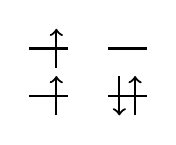
\begin{tikzpicture}[baseline={(current bounding box.center)}]
    % oberste MOs:
    \draw[thick] (0,0) -- (0.5,0); % erster Strich
    \draw[thick] (1,0) -- (1.5,0); % zweiter Strich
    % unterste MOs:
    \draw[thick] (0,-0.6) -- (0.5,-0.6); % dritter Strich
    \draw[thick] (1,-0.6) -- (1.5,-0.6); % vierter Strich
\draw[->, thick] (0.35, -0.25) -- (0.35, 0.25); 
\draw[-> , thick] (0.35, -0.85) -- (0.35, -0.35); 
 \draw[-> , thick] (1.35, -0.85) -- (1.35, -0.35); 
\draw[<- , thick] (1.15, -0.85) -- (1.15, -0.35); 
\end{tikzpicture}\qquad 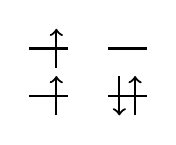
\begin{tikzpicture}[baseline={(current bounding box.center)}]
    % oberste MOs:
    \draw[thick] (0,0) -- (0.5,0); % erster Strich
    \draw[thick] (1,0) -- (1.5,0); % zweiter Strich
    % unterste MOs:
    \draw[thick] (0,-0.6) -- (0.5,-0.6); % dritter Strich
    \draw[thick] (1,-0.6) -- (1.5,-0.6); % vierter Strich
\draw[->, thick] (0.35, -0.25) -- (0.35, 0.25); 
\draw[-> , thick] (0.35, -0.85) -- (0.35, -0.35); 
 \draw[-> , thick] (1.35, -0.85) -- (1.35, -0.35); 
\draw[<- , thick] (1.15, -0.85) -- (1.15, -0.35); 
\end{tikzpicture}}\right)-\left(\text{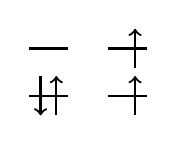
\begin{tikzpicture}[baseline={(current bounding box.center)}]
    % oberste MOs:
    \draw[thick] (0,0) -- (0.5,0); % erster Strich
    \draw[thick] (1,0) -- (1.5,0); % zweiter Strich
    % unterste MOs:
    \draw[thick] (0,-0.6) -- (0.5,-0.6); % dritter Strich
    \draw[thick] (1,-0.6) -- (1.5,-0.6); % vierter Strich
\draw[->, thick] (1.35, -0.25) -- (1.35, 0.25); 
\draw[-> , thick] (0.35, -0.85) -- (0.35, -0.35); 
\draw[<- , thick] (0.15, -0.85) -- (0.15, -0.35); 
 \draw[-> , thick] (1.35, -0.85) -- (1.35, -0.35); 
\end{tikzpicture}\qquad 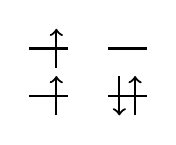
\begin{tikzpicture}[baseline={(current bounding box.center)}]
    % oberste MOs:
    \draw[thick] (0,0) -- (0.5,0); % erster Strich
    \draw[thick] (1,0) -- (1.5,0); % zweiter Strich
    % unterste MOs:
    \draw[thick] (0,-0.6) -- (0.5,-0.6); % dritter Strich
    \draw[thick] (1,-0.6) -- (1.5,-0.6); % vierter Strich
\draw[->, thick] (0.35, -0.25) -- (0.35, 0.25); 
\draw[-> , thick] (0.35, -0.85) -- (0.35, -0.35); 
 \draw[-> , thick] (1.35, -0.85) -- (1.35, -0.35); 
\draw[<- , thick] (1.15, -0.85) -- (1.15, -0.35); 
\end{tikzpicture}}\right)-\left(\text{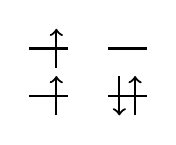
\begin{tikzpicture}[baseline={(current bounding box.center)}]
    % oberste MOs:
    \draw[thick] (0,0) -- (0.5,0); % erster Strich
    \draw[thick] (1,0) -- (1.5,0); % zweiter Strich
    % unterste MOs:
    \draw[thick] (0,-0.6) -- (0.5,-0.6); % dritter Strich
    \draw[thick] (1,-0.6) -- (1.5,-0.6); % vierter Strich
\draw[->, thick] (0.35, -0.25) -- (0.35, 0.25); 
\draw[-> , thick] (0.35, -0.85) -- (0.35, -0.35); 
 \draw[-> , thick] (1.35, -0.85) -- (1.35, -0.35); 
\draw[<- , thick] (1.15, -0.85) -- (1.15, -0.35); 
\end{tikzpicture}\qquad 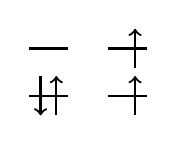
\begin{tikzpicture}[baseline={(current bounding box.center)}]
    % oberste MOs:
    \draw[thick] (0,0) -- (0.5,0); % erster Strich
    \draw[thick] (1,0) -- (1.5,0); % zweiter Strich
    % unterste MOs:
    \draw[thick] (0,-0.6) -- (0.5,-0.6); % dritter Strich
    \draw[thick] (1,-0.6) -- (1.5,-0.6); % vierter Strich
\draw[->, thick] (1.35, -0.25) -- (1.35, 0.25); 
\draw[-> , thick] (0.35, -0.85) -- (0.35, -0.35); 
\draw[<- , thick] (0.15, -0.85) -- (0.15, -0.35); 
 \draw[-> , thick] (1.35, -0.85) -- (1.35, -0.35); 
\end{tikzpicture}}\right)+\left(\text{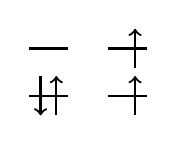
\begin{tikzpicture}[baseline={(current bounding box.center)}]
    % oberste MOs:
    \draw[thick] (0,0) -- (0.5,0); % erster Strich
    \draw[thick] (1,0) -- (1.5,0); % zweiter Strich
    % unterste MOs:
    \draw[thick] (0,-0.6) -- (0.5,-0.6); % dritter Strich
    \draw[thick] (1,-0.6) -- (1.5,-0.6); % vierter Strich
\draw[->, thick] (1.35, -0.25) -- (1.35, 0.25); 
\draw[-> , thick] (0.35, -0.85) -- (0.35, -0.35); 
\draw[<- , thick] (0.15, -0.85) -- (0.15, -0.35); 
 \draw[-> , thick] (1.35, -0.85) -- (1.35, -0.35); 
\end{tikzpicture}\qquad 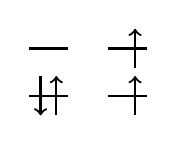
\begin{tikzpicture}[baseline={(current bounding box.center)}]
    % oberste MOs:
    \draw[thick] (0,0) -- (0.5,0); % erster Strich
    \draw[thick] (1,0) -- (1.5,0); % zweiter Strich
    % unterste MOs:
    \draw[thick] (0,-0.6) -- (0.5,-0.6); % dritter Strich
    \draw[thick] (1,-0.6) -- (1.5,-0.6); % vierter Strich
\draw[->, thick] (1.35, -0.25) -- (1.35, 0.25); 
\draw[-> , thick] (0.35, -0.85) -- (0.35, -0.35); 
\draw[<- , thick] (0.15, -0.85) -- (0.15, -0.35); 
 \draw[-> , thick] (1.35, -0.85) -- (1.35, -0.35); 
\end{tikzpicture}}\right)\\\\\]


bzw. in CI-Vektoren geschrieben: 
 $$+ 1 \cdot \left|aa20 \right| \cdot \left| aa20 \right| 
- 1 \cdot \left|02aa \right| \cdot \left| aa20 \right| 
- 1 \cdot \left|aa20 \right| \cdot \left| 02aa \right| 
+ 1 \cdot \left|02aa \right| \cdot \left| 02aa \right| 
$$



 bildet folgende mögliche Dimerkombinationen:

$$+ 1 \cdot \left|aa20aa20 \right| + 1 \cdot \left|02aa02aa \right| - \frac{1}{8} \cdot \left|02aaaa20 \right| - \frac{1}{8} \cdot \left|02a0aa2a \right| - \frac{1}{8} \cdot \left|022aaaa0 \right| - \frac{1}{8} \cdot \left|0220aaaa \right|  $$ $$ - \frac{1}{8} \cdot \left|0aaaa220 \right| - \frac{1}{8} \cdot \left|0aa0a22a \right| - \frac{1}{8} \cdot \left|0a2aa2a0 \right| - \frac{1}{8} \cdot \left|0a20a2aa \right| - \frac{1}{8} \cdot \left|a2aa0a20 \right| - \frac{1}{8} \cdot \left|a2a00a2a \right|  $$ $$ - \frac{1}{8} \cdot \left|a22a0aa0 \right| - \frac{1}{8} \cdot \left|a2200aaa \right| - \frac{1}{8} \cdot \left|aaaa0220 \right| - \frac{1}{8} \cdot \left|aaa0022a \right| - \frac{1}{8} \cdot \left|aa2a02a0 \right| - \frac{1}{8} \cdot \left|aa2002aa \right| $$



\end{minipage}
\vspace{0.5cm}
\hrule
\vspace{0.5cm}



\begin{minipage}{\linewidth}
$i^3 b_{2u}$ * $e^3 b_{2u}$ \quad = \quad $1.3$ * $2.3$
\[ +\left(\text{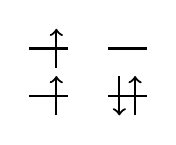
\begin{tikzpicture}[baseline={(current bounding box.center)}]
    % oberste MOs:
    \draw[thick] (0,0) -- (0.5,0); % erster Strich
    \draw[thick] (1,0) -- (1.5,0); % zweiter Strich
    % unterste MOs:
    \draw[thick] (0,-0.6) -- (0.5,-0.6); % dritter Strich
    \draw[thick] (1,-0.6) -- (1.5,-0.6); % vierter Strich
\draw[->, thick] (0.35, -0.25) -- (0.35, 0.25); 
\draw[-> , thick] (0.35, -0.85) -- (0.35, -0.35); 
 \draw[-> , thick] (1.35, -0.85) -- (1.35, -0.35); 
\draw[<- , thick] (1.15, -0.85) -- (1.15, -0.35); 
\end{tikzpicture}\qquad 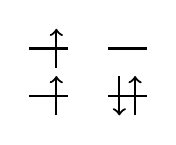
\begin{tikzpicture}[baseline={(current bounding box.center)}]
    % oberste MOs:
    \draw[thick] (0,0) -- (0.5,0); % erster Strich
    \draw[thick] (1,0) -- (1.5,0); % zweiter Strich
    % unterste MOs:
    \draw[thick] (0,-0.6) -- (0.5,-0.6); % dritter Strich
    \draw[thick] (1,-0.6) -- (1.5,-0.6); % vierter Strich
\draw[->, thick] (0.35, -0.25) -- (0.35, 0.25); 
\draw[-> , thick] (0.35, -0.85) -- (0.35, -0.35); 
 \draw[-> , thick] (1.35, -0.85) -- (1.35, -0.35); 
\draw[<- , thick] (1.15, -0.85) -- (1.15, -0.35); 
\end{tikzpicture}}\right)-\left(\text{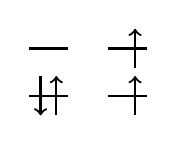
\begin{tikzpicture}[baseline={(current bounding box.center)}]
    % oberste MOs:
    \draw[thick] (0,0) -- (0.5,0); % erster Strich
    \draw[thick] (1,0) -- (1.5,0); % zweiter Strich
    % unterste MOs:
    \draw[thick] (0,-0.6) -- (0.5,-0.6); % dritter Strich
    \draw[thick] (1,-0.6) -- (1.5,-0.6); % vierter Strich
\draw[->, thick] (1.35, -0.25) -- (1.35, 0.25); 
\draw[-> , thick] (0.35, -0.85) -- (0.35, -0.35); 
\draw[<- , thick] (0.15, -0.85) -- (0.15, -0.35); 
 \draw[-> , thick] (1.35, -0.85) -- (1.35, -0.35); 
\end{tikzpicture}\qquad 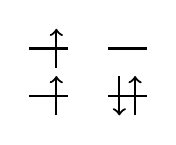
\begin{tikzpicture}[baseline={(current bounding box.center)}]
    % oberste MOs:
    \draw[thick] (0,0) -- (0.5,0); % erster Strich
    \draw[thick] (1,0) -- (1.5,0); % zweiter Strich
    % unterste MOs:
    \draw[thick] (0,-0.6) -- (0.5,-0.6); % dritter Strich
    \draw[thick] (1,-0.6) -- (1.5,-0.6); % vierter Strich
\draw[->, thick] (0.35, -0.25) -- (0.35, 0.25); 
\draw[-> , thick] (0.35, -0.85) -- (0.35, -0.35); 
 \draw[-> , thick] (1.35, -0.85) -- (1.35, -0.35); 
\draw[<- , thick] (1.15, -0.85) -- (1.15, -0.35); 
\end{tikzpicture}}\right)+\left(\text{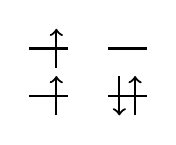
\begin{tikzpicture}[baseline={(current bounding box.center)}]
    % oberste MOs:
    \draw[thick] (0,0) -- (0.5,0); % erster Strich
    \draw[thick] (1,0) -- (1.5,0); % zweiter Strich
    % unterste MOs:
    \draw[thick] (0,-0.6) -- (0.5,-0.6); % dritter Strich
    \draw[thick] (1,-0.6) -- (1.5,-0.6); % vierter Strich
\draw[->, thick] (0.35, -0.25) -- (0.35, 0.25); 
\draw[-> , thick] (0.35, -0.85) -- (0.35, -0.35); 
 \draw[-> , thick] (1.35, -0.85) -- (1.35, -0.35); 
\draw[<- , thick] (1.15, -0.85) -- (1.15, -0.35); 
\end{tikzpicture}\qquad 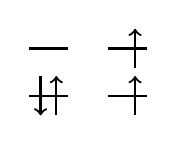
\begin{tikzpicture}[baseline={(current bounding box.center)}]
    % oberste MOs:
    \draw[thick] (0,0) -- (0.5,0); % erster Strich
    \draw[thick] (1,0) -- (1.5,0); % zweiter Strich
    % unterste MOs:
    \draw[thick] (0,-0.6) -- (0.5,-0.6); % dritter Strich
    \draw[thick] (1,-0.6) -- (1.5,-0.6); % vierter Strich
\draw[->, thick] (1.35, -0.25) -- (1.35, 0.25); 
\draw[-> , thick] (0.35, -0.85) -- (0.35, -0.35); 
\draw[<- , thick] (0.15, -0.85) -- (0.15, -0.35); 
 \draw[-> , thick] (1.35, -0.85) -- (1.35, -0.35); 
\end{tikzpicture}}\right)-\left(\text{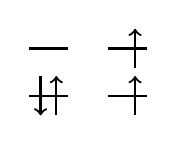
\begin{tikzpicture}[baseline={(current bounding box.center)}]
    % oberste MOs:
    \draw[thick] (0,0) -- (0.5,0); % erster Strich
    \draw[thick] (1,0) -- (1.5,0); % zweiter Strich
    % unterste MOs:
    \draw[thick] (0,-0.6) -- (0.5,-0.6); % dritter Strich
    \draw[thick] (1,-0.6) -- (1.5,-0.6); % vierter Strich
\draw[->, thick] (1.35, -0.25) -- (1.35, 0.25); 
\draw[-> , thick] (0.35, -0.85) -- (0.35, -0.35); 
\draw[<- , thick] (0.15, -0.85) -- (0.15, -0.35); 
 \draw[-> , thick] (1.35, -0.85) -- (1.35, -0.35); 
\end{tikzpicture}\qquad 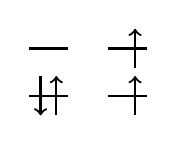
\begin{tikzpicture}[baseline={(current bounding box.center)}]
    % oberste MOs:
    \draw[thick] (0,0) -- (0.5,0); % erster Strich
    \draw[thick] (1,0) -- (1.5,0); % zweiter Strich
    % unterste MOs:
    \draw[thick] (0,-0.6) -- (0.5,-0.6); % dritter Strich
    \draw[thick] (1,-0.6) -- (1.5,-0.6); % vierter Strich
\draw[->, thick] (1.35, -0.25) -- (1.35, 0.25); 
\draw[-> , thick] (0.35, -0.85) -- (0.35, -0.35); 
\draw[<- , thick] (0.15, -0.85) -- (0.15, -0.35); 
 \draw[-> , thick] (1.35, -0.85) -- (1.35, -0.35); 
\end{tikzpicture}}\right)\\\\\]


bzw. in CI-Vektoren geschrieben: 
 $$+ 1 \cdot \left|aa20 \right| \cdot \left| aa20 \right| 
- 1 \cdot \left|02aa \right| \cdot \left| aa20 \right| 
+ 1 \cdot \left|aa20 \right| \cdot \left| 02aa \right| 
- 1 \cdot \left|02aa \right| \cdot \left| 02aa \right| 
$$



 bildet folgende mögliche Dimerkombinationen:

$$+ 1 \cdot \left|aa20aa20 \right| - 1 \cdot \left|02aa02aa \right| $$



\end{minipage}
\vspace{0.5cm}
\hrule
\vspace{0.5cm}



\begin{minipage}{\linewidth}
$i^3 b_{2u}$ * $e^3 b_{3u}$ \quad = \quad $1.3$ * $1.2$
\[ +\left(\text{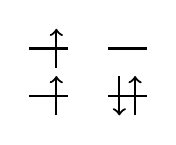
\begin{tikzpicture}[baseline={(current bounding box.center)}]
    % oberste MOs:
    \draw[thick] (0,0) -- (0.5,0); % erster Strich
    \draw[thick] (1,0) -- (1.5,0); % zweiter Strich
    % unterste MOs:
    \draw[thick] (0,-0.6) -- (0.5,-0.6); % dritter Strich
    \draw[thick] (1,-0.6) -- (1.5,-0.6); % vierter Strich
\draw[->, thick] (0.35, -0.25) -- (0.35, 0.25); 
\draw[-> , thick] (0.35, -0.85) -- (0.35, -0.35); 
 \draw[-> , thick] (1.35, -0.85) -- (1.35, -0.35); 
\draw[<- , thick] (1.15, -0.85) -- (1.15, -0.35); 
\end{tikzpicture}\qquad 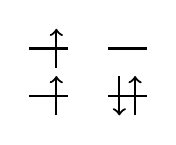
\begin{tikzpicture}[baseline={(current bounding box.center)}]
    % oberste MOs:
    \draw[thick] (0,0) -- (0.5,0); % erster Strich
    \draw[thick] (1,0) -- (1.5,0); % zweiter Strich
    % unterste MOs:
    \draw[thick] (0,-0.6) -- (0.5,-0.6); % dritter Strich
    \draw[thick] (1,-0.6) -- (1.5,-0.6); % vierter Strich
\draw[->, thick] (0.35, -0.25) -- (0.35, 0.25); 
\draw[-> , thick] (0.35, -0.85) -- (0.35, -0.35); 
 \draw[-> , thick] (1.35, -0.85) -- (1.35, -0.35); 
\draw[<- , thick] (1.15, -0.85) -- (1.15, -0.35); 
\end{tikzpicture}}\right)-\left(\text{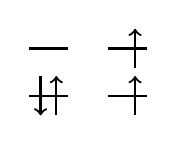
\begin{tikzpicture}[baseline={(current bounding box.center)}]
    % oberste MOs:
    \draw[thick] (0,0) -- (0.5,0); % erster Strich
    \draw[thick] (1,0) -- (1.5,0); % zweiter Strich
    % unterste MOs:
    \draw[thick] (0,-0.6) -- (0.5,-0.6); % dritter Strich
    \draw[thick] (1,-0.6) -- (1.5,-0.6); % vierter Strich
\draw[->, thick] (1.35, -0.25) -- (1.35, 0.25); 
\draw[-> , thick] (0.35, -0.85) -- (0.35, -0.35); 
\draw[<- , thick] (0.15, -0.85) -- (0.15, -0.35); 
 \draw[-> , thick] (1.35, -0.85) -- (1.35, -0.35); 
\end{tikzpicture}\qquad 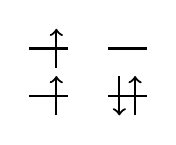
\begin{tikzpicture}[baseline={(current bounding box.center)}]
    % oberste MOs:
    \draw[thick] (0,0) -- (0.5,0); % erster Strich
    \draw[thick] (1,0) -- (1.5,0); % zweiter Strich
    % unterste MOs:
    \draw[thick] (0,-0.6) -- (0.5,-0.6); % dritter Strich
    \draw[thick] (1,-0.6) -- (1.5,-0.6); % vierter Strich
\draw[->, thick] (0.35, -0.25) -- (0.35, 0.25); 
\draw[-> , thick] (0.35, -0.85) -- (0.35, -0.35); 
 \draw[-> , thick] (1.35, -0.85) -- (1.35, -0.35); 
\draw[<- , thick] (1.15, -0.85) -- (1.15, -0.35); 
\end{tikzpicture}}\right)-\left(\text{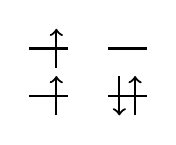
\begin{tikzpicture}[baseline={(current bounding box.center)}]
    % oberste MOs:
    \draw[thick] (0,0) -- (0.5,0); % erster Strich
    \draw[thick] (1,0) -- (1.5,0); % zweiter Strich
    % unterste MOs:
    \draw[thick] (0,-0.6) -- (0.5,-0.6); % dritter Strich
    \draw[thick] (1,-0.6) -- (1.5,-0.6); % vierter Strich
\draw[->, thick] (0.35, -0.25) -- (0.35, 0.25); 
\draw[-> , thick] (0.35, -0.85) -- (0.35, -0.35); 
 \draw[-> , thick] (1.35, -0.85) -- (1.35, -0.35); 
\draw[<- , thick] (1.15, -0.85) -- (1.15, -0.35); 
\end{tikzpicture}\qquad 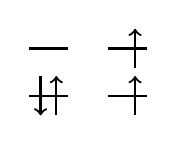
\begin{tikzpicture}[baseline={(current bounding box.center)}]
    % oberste MOs:
    \draw[thick] (0,0) -- (0.5,0); % erster Strich
    \draw[thick] (1,0) -- (1.5,0); % zweiter Strich
    % unterste MOs:
    \draw[thick] (0,-0.6) -- (0.5,-0.6); % dritter Strich
    \draw[thick] (1,-0.6) -- (1.5,-0.6); % vierter Strich
\draw[->, thick] (1.35, -0.25) -- (1.35, 0.25); 
\draw[-> , thick] (0.35, -0.85) -- (0.35, -0.35); 
\draw[<- , thick] (0.15, -0.85) -- (0.15, -0.35); 
 \draw[-> , thick] (1.35, -0.85) -- (1.35, -0.35); 
\end{tikzpicture}}\right)+\left(\text{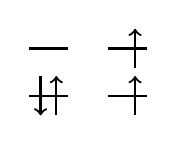
\begin{tikzpicture}[baseline={(current bounding box.center)}]
    % oberste MOs:
    \draw[thick] (0,0) -- (0.5,0); % erster Strich
    \draw[thick] (1,0) -- (1.5,0); % zweiter Strich
    % unterste MOs:
    \draw[thick] (0,-0.6) -- (0.5,-0.6); % dritter Strich
    \draw[thick] (1,-0.6) -- (1.5,-0.6); % vierter Strich
\draw[->, thick] (1.35, -0.25) -- (1.35, 0.25); 
\draw[-> , thick] (0.35, -0.85) -- (0.35, -0.35); 
\draw[<- , thick] (0.15, -0.85) -- (0.15, -0.35); 
 \draw[-> , thick] (1.35, -0.85) -- (1.35, -0.35); 
\end{tikzpicture}\qquad 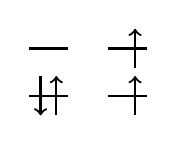
\begin{tikzpicture}[baseline={(current bounding box.center)}]
    % oberste MOs:
    \draw[thick] (0,0) -- (0.5,0); % erster Strich
    \draw[thick] (1,0) -- (1.5,0); % zweiter Strich
    % unterste MOs:
    \draw[thick] (0,-0.6) -- (0.5,-0.6); % dritter Strich
    \draw[thick] (1,-0.6) -- (1.5,-0.6); % vierter Strich
\draw[->, thick] (1.35, -0.25) -- (1.35, 0.25); 
\draw[-> , thick] (0.35, -0.85) -- (0.35, -0.35); 
\draw[<- , thick] (0.15, -0.85) -- (0.15, -0.35); 
 \draw[-> , thick] (1.35, -0.85) -- (1.35, -0.35); 
\end{tikzpicture}}\right)\\\\\]


bzw. in CI-Vektoren geschrieben: 
 $$+ 1 \cdot \left|aa20 \right| \cdot \left| aa20 \right| 
- 1 \cdot \left|02aa \right| \cdot \left| aa20 \right| 
- 1 \cdot \left|aa20 \right| \cdot \left| 02aa \right| 
+ 1 \cdot \left|02aa \right| \cdot \left| 02aa \right| 
$$



 bildet folgende mögliche Dimerkombinationen:

$$+ 1 \cdot \left|aa20aa20 \right| + 1 \cdot \left|02aa02aa \right| - \frac{1}{8} \cdot \left|02aaaa20 \right| - \frac{1}{8} \cdot \left|02a0aa2a \right| - \frac{1}{8} \cdot \left|022aaaa0 \right| - \frac{1}{8} \cdot \left|0220aaaa \right|  $$ $$ - \frac{1}{8} \cdot \left|0aaaa220 \right| - \frac{1}{8} \cdot \left|0aa0a22a \right| - \frac{1}{8} \cdot \left|0a2aa2a0 \right| - \frac{1}{8} \cdot \left|0a20a2aa \right| - \frac{1}{8} \cdot \left|a2aa0a20 \right| - \frac{1}{8} \cdot \left|a2a00a2a \right|  $$ $$ - \frac{1}{8} \cdot \left|a22a0aa0 \right| - \frac{1}{8} \cdot \left|a2200aaa \right| - \frac{1}{8} \cdot \left|aaaa0220 \right| - \frac{1}{8} \cdot \left|aaa0022a \right| - \frac{1}{8} \cdot \left|aa2a02a0 \right| - \frac{1}{8} \cdot \left|aa2002aa \right| $$



\end{minipage}
\vspace{0.5cm}
\hrule
\vspace{0.5cm}



\begin{minipage}{\linewidth}
$i^3 b_{2u}$ * $i^3 b_{3u}$ \quad = \quad $1.3$ * $2.2$
\[ +\left(\text{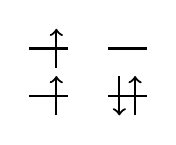
\begin{tikzpicture}[baseline={(current bounding box.center)}]
    % oberste MOs:
    \draw[thick] (0,0) -- (0.5,0); % erster Strich
    \draw[thick] (1,0) -- (1.5,0); % zweiter Strich
    % unterste MOs:
    \draw[thick] (0,-0.6) -- (0.5,-0.6); % dritter Strich
    \draw[thick] (1,-0.6) -- (1.5,-0.6); % vierter Strich
\draw[->, thick] (0.35, -0.25) -- (0.35, 0.25); 
\draw[-> , thick] (0.35, -0.85) -- (0.35, -0.35); 
 \draw[-> , thick] (1.35, -0.85) -- (1.35, -0.35); 
\draw[<- , thick] (1.15, -0.85) -- (1.15, -0.35); 
\end{tikzpicture}\qquad 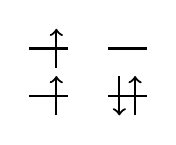
\begin{tikzpicture}[baseline={(current bounding box.center)}]
    % oberste MOs:
    \draw[thick] (0,0) -- (0.5,0); % erster Strich
    \draw[thick] (1,0) -- (1.5,0); % zweiter Strich
    % unterste MOs:
    \draw[thick] (0,-0.6) -- (0.5,-0.6); % dritter Strich
    \draw[thick] (1,-0.6) -- (1.5,-0.6); % vierter Strich
\draw[->, thick] (0.35, -0.25) -- (0.35, 0.25); 
\draw[-> , thick] (0.35, -0.85) -- (0.35, -0.35); 
 \draw[-> , thick] (1.35, -0.85) -- (1.35, -0.35); 
\draw[<- , thick] (1.15, -0.85) -- (1.15, -0.35); 
\end{tikzpicture}}\right)-\left(\text{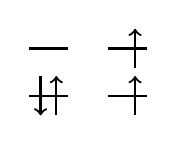
\begin{tikzpicture}[baseline={(current bounding box.center)}]
    % oberste MOs:
    \draw[thick] (0,0) -- (0.5,0); % erster Strich
    \draw[thick] (1,0) -- (1.5,0); % zweiter Strich
    % unterste MOs:
    \draw[thick] (0,-0.6) -- (0.5,-0.6); % dritter Strich
    \draw[thick] (1,-0.6) -- (1.5,-0.6); % vierter Strich
\draw[->, thick] (1.35, -0.25) -- (1.35, 0.25); 
\draw[-> , thick] (0.35, -0.85) -- (0.35, -0.35); 
\draw[<- , thick] (0.15, -0.85) -- (0.15, -0.35); 
 \draw[-> , thick] (1.35, -0.85) -- (1.35, -0.35); 
\end{tikzpicture}\qquad 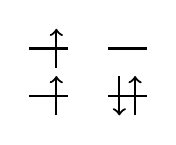
\begin{tikzpicture}[baseline={(current bounding box.center)}]
    % oberste MOs:
    \draw[thick] (0,0) -- (0.5,0); % erster Strich
    \draw[thick] (1,0) -- (1.5,0); % zweiter Strich
    % unterste MOs:
    \draw[thick] (0,-0.6) -- (0.5,-0.6); % dritter Strich
    \draw[thick] (1,-0.6) -- (1.5,-0.6); % vierter Strich
\draw[->, thick] (0.35, -0.25) -- (0.35, 0.25); 
\draw[-> , thick] (0.35, -0.85) -- (0.35, -0.35); 
 \draw[-> , thick] (1.35, -0.85) -- (1.35, -0.35); 
\draw[<- , thick] (1.15, -0.85) -- (1.15, -0.35); 
\end{tikzpicture}}\right)+\left(\text{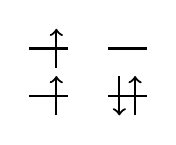
\begin{tikzpicture}[baseline={(current bounding box.center)}]
    % oberste MOs:
    \draw[thick] (0,0) -- (0.5,0); % erster Strich
    \draw[thick] (1,0) -- (1.5,0); % zweiter Strich
    % unterste MOs:
    \draw[thick] (0,-0.6) -- (0.5,-0.6); % dritter Strich
    \draw[thick] (1,-0.6) -- (1.5,-0.6); % vierter Strich
\draw[->, thick] (0.35, -0.25) -- (0.35, 0.25); 
\draw[-> , thick] (0.35, -0.85) -- (0.35, -0.35); 
 \draw[-> , thick] (1.35, -0.85) -- (1.35, -0.35); 
\draw[<- , thick] (1.15, -0.85) -- (1.15, -0.35); 
\end{tikzpicture}\qquad 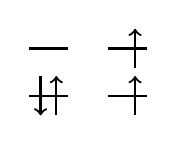
\begin{tikzpicture}[baseline={(current bounding box.center)}]
    % oberste MOs:
    \draw[thick] (0,0) -- (0.5,0); % erster Strich
    \draw[thick] (1,0) -- (1.5,0); % zweiter Strich
    % unterste MOs:
    \draw[thick] (0,-0.6) -- (0.5,-0.6); % dritter Strich
    \draw[thick] (1,-0.6) -- (1.5,-0.6); % vierter Strich
\draw[->, thick] (1.35, -0.25) -- (1.35, 0.25); 
\draw[-> , thick] (0.35, -0.85) -- (0.35, -0.35); 
\draw[<- , thick] (0.15, -0.85) -- (0.15, -0.35); 
 \draw[-> , thick] (1.35, -0.85) -- (1.35, -0.35); 
\end{tikzpicture}}\right)-\left(\text{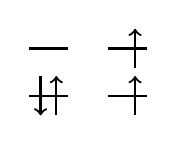
\begin{tikzpicture}[baseline={(current bounding box.center)}]
    % oberste MOs:
    \draw[thick] (0,0) -- (0.5,0); % erster Strich
    \draw[thick] (1,0) -- (1.5,0); % zweiter Strich
    % unterste MOs:
    \draw[thick] (0,-0.6) -- (0.5,-0.6); % dritter Strich
    \draw[thick] (1,-0.6) -- (1.5,-0.6); % vierter Strich
\draw[->, thick] (1.35, -0.25) -- (1.35, 0.25); 
\draw[-> , thick] (0.35, -0.85) -- (0.35, -0.35); 
\draw[<- , thick] (0.15, -0.85) -- (0.15, -0.35); 
 \draw[-> , thick] (1.35, -0.85) -- (1.35, -0.35); 
\end{tikzpicture}\qquad 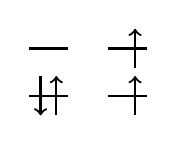
\begin{tikzpicture}[baseline={(current bounding box.center)}]
    % oberste MOs:
    \draw[thick] (0,0) -- (0.5,0); % erster Strich
    \draw[thick] (1,0) -- (1.5,0); % zweiter Strich
    % unterste MOs:
    \draw[thick] (0,-0.6) -- (0.5,-0.6); % dritter Strich
    \draw[thick] (1,-0.6) -- (1.5,-0.6); % vierter Strich
\draw[->, thick] (1.35, -0.25) -- (1.35, 0.25); 
\draw[-> , thick] (0.35, -0.85) -- (0.35, -0.35); 
\draw[<- , thick] (0.15, -0.85) -- (0.15, -0.35); 
 \draw[-> , thick] (1.35, -0.85) -- (1.35, -0.35); 
\end{tikzpicture}}\right)\\\\\]


bzw. in CI-Vektoren geschrieben: 
 $$+ 1 \cdot \left|aa20 \right| \cdot \left| aa20 \right| 
- 1 \cdot \left|02aa \right| \cdot \left| aa20 \right| 
+ 1 \cdot \left|aa20 \right| \cdot \left| 02aa \right| 
- 1 \cdot \left|02aa \right| \cdot \left| 02aa \right| 
$$



 bildet folgende mögliche Dimerkombinationen:

$$+ 1 \cdot \left|aa20aa20 \right| - 1 \cdot \left|02aa02aa \right| $$



\end{minipage}
\vspace{0.5cm}
\hrule
\vspace{0.5cm}



\begin{minipage}{\linewidth}
$e^3 b_{2u}$ * $i^3 b_{2u}$ \quad = \quad $2.3$ * $1.3$
\[ +\left(\text{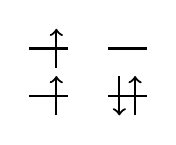
\begin{tikzpicture}[baseline={(current bounding box.center)}]
    % oberste MOs:
    \draw[thick] (0,0) -- (0.5,0); % erster Strich
    \draw[thick] (1,0) -- (1.5,0); % zweiter Strich
    % unterste MOs:
    \draw[thick] (0,-0.6) -- (0.5,-0.6); % dritter Strich
    \draw[thick] (1,-0.6) -- (1.5,-0.6); % vierter Strich
\draw[->, thick] (0.35, -0.25) -- (0.35, 0.25); 
\draw[-> , thick] (0.35, -0.85) -- (0.35, -0.35); 
 \draw[-> , thick] (1.35, -0.85) -- (1.35, -0.35); 
\draw[<- , thick] (1.15, -0.85) -- (1.15, -0.35); 
\end{tikzpicture}\qquad 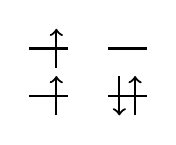
\begin{tikzpicture}[baseline={(current bounding box.center)}]
    % oberste MOs:
    \draw[thick] (0,0) -- (0.5,0); % erster Strich
    \draw[thick] (1,0) -- (1.5,0); % zweiter Strich
    % unterste MOs:
    \draw[thick] (0,-0.6) -- (0.5,-0.6); % dritter Strich
    \draw[thick] (1,-0.6) -- (1.5,-0.6); % vierter Strich
\draw[->, thick] (0.35, -0.25) -- (0.35, 0.25); 
\draw[-> , thick] (0.35, -0.85) -- (0.35, -0.35); 
 \draw[-> , thick] (1.35, -0.85) -- (1.35, -0.35); 
\draw[<- , thick] (1.15, -0.85) -- (1.15, -0.35); 
\end{tikzpicture}}\right)+\left(\text{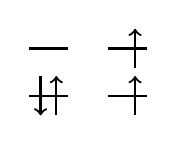
\begin{tikzpicture}[baseline={(current bounding box.center)}]
    % oberste MOs:
    \draw[thick] (0,0) -- (0.5,0); % erster Strich
    \draw[thick] (1,0) -- (1.5,0); % zweiter Strich
    % unterste MOs:
    \draw[thick] (0,-0.6) -- (0.5,-0.6); % dritter Strich
    \draw[thick] (1,-0.6) -- (1.5,-0.6); % vierter Strich
\draw[->, thick] (1.35, -0.25) -- (1.35, 0.25); 
\draw[-> , thick] (0.35, -0.85) -- (0.35, -0.35); 
\draw[<- , thick] (0.15, -0.85) -- (0.15, -0.35); 
 \draw[-> , thick] (1.35, -0.85) -- (1.35, -0.35); 
\end{tikzpicture}\qquad 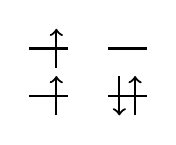
\begin{tikzpicture}[baseline={(current bounding box.center)}]
    % oberste MOs:
    \draw[thick] (0,0) -- (0.5,0); % erster Strich
    \draw[thick] (1,0) -- (1.5,0); % zweiter Strich
    % unterste MOs:
    \draw[thick] (0,-0.6) -- (0.5,-0.6); % dritter Strich
    \draw[thick] (1,-0.6) -- (1.5,-0.6); % vierter Strich
\draw[->, thick] (0.35, -0.25) -- (0.35, 0.25); 
\draw[-> , thick] (0.35, -0.85) -- (0.35, -0.35); 
 \draw[-> , thick] (1.35, -0.85) -- (1.35, -0.35); 
\draw[<- , thick] (1.15, -0.85) -- (1.15, -0.35); 
\end{tikzpicture}}\right)-\left(\text{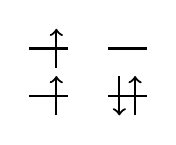
\begin{tikzpicture}[baseline={(current bounding box.center)}]
    % oberste MOs:
    \draw[thick] (0,0) -- (0.5,0); % erster Strich
    \draw[thick] (1,0) -- (1.5,0); % zweiter Strich
    % unterste MOs:
    \draw[thick] (0,-0.6) -- (0.5,-0.6); % dritter Strich
    \draw[thick] (1,-0.6) -- (1.5,-0.6); % vierter Strich
\draw[->, thick] (0.35, -0.25) -- (0.35, 0.25); 
\draw[-> , thick] (0.35, -0.85) -- (0.35, -0.35); 
 \draw[-> , thick] (1.35, -0.85) -- (1.35, -0.35); 
\draw[<- , thick] (1.15, -0.85) -- (1.15, -0.35); 
\end{tikzpicture}\qquad 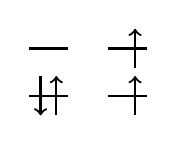
\begin{tikzpicture}[baseline={(current bounding box.center)}]
    % oberste MOs:
    \draw[thick] (0,0) -- (0.5,0); % erster Strich
    \draw[thick] (1,0) -- (1.5,0); % zweiter Strich
    % unterste MOs:
    \draw[thick] (0,-0.6) -- (0.5,-0.6); % dritter Strich
    \draw[thick] (1,-0.6) -- (1.5,-0.6); % vierter Strich
\draw[->, thick] (1.35, -0.25) -- (1.35, 0.25); 
\draw[-> , thick] (0.35, -0.85) -- (0.35, -0.35); 
\draw[<- , thick] (0.15, -0.85) -- (0.15, -0.35); 
 \draw[-> , thick] (1.35, -0.85) -- (1.35, -0.35); 
\end{tikzpicture}}\right)-\left(\text{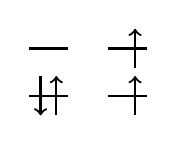
\begin{tikzpicture}[baseline={(current bounding box.center)}]
    % oberste MOs:
    \draw[thick] (0,0) -- (0.5,0); % erster Strich
    \draw[thick] (1,0) -- (1.5,0); % zweiter Strich
    % unterste MOs:
    \draw[thick] (0,-0.6) -- (0.5,-0.6); % dritter Strich
    \draw[thick] (1,-0.6) -- (1.5,-0.6); % vierter Strich
\draw[->, thick] (1.35, -0.25) -- (1.35, 0.25); 
\draw[-> , thick] (0.35, -0.85) -- (0.35, -0.35); 
\draw[<- , thick] (0.15, -0.85) -- (0.15, -0.35); 
 \draw[-> , thick] (1.35, -0.85) -- (1.35, -0.35); 
\end{tikzpicture}\qquad 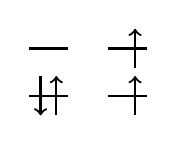
\begin{tikzpicture}[baseline={(current bounding box.center)}]
    % oberste MOs:
    \draw[thick] (0,0) -- (0.5,0); % erster Strich
    \draw[thick] (1,0) -- (1.5,0); % zweiter Strich
    % unterste MOs:
    \draw[thick] (0,-0.6) -- (0.5,-0.6); % dritter Strich
    \draw[thick] (1,-0.6) -- (1.5,-0.6); % vierter Strich
\draw[->, thick] (1.35, -0.25) -- (1.35, 0.25); 
\draw[-> , thick] (0.35, -0.85) -- (0.35, -0.35); 
\draw[<- , thick] (0.15, -0.85) -- (0.15, -0.35); 
 \draw[-> , thick] (1.35, -0.85) -- (1.35, -0.35); 
\end{tikzpicture}}\right)\\\\\]


bzw. in CI-Vektoren geschrieben: 
 $$+ 1 \cdot \left|aa20 \right| \cdot \left| aa20 \right| 
+ 1 \cdot \left|02aa \right| \cdot \left| aa20 \right| 
- 1 \cdot \left|aa20 \right| \cdot \left| 02aa \right| 
- 1 \cdot \left|02aa \right| \cdot \left| 02aa \right| 
$$



 bildet folgende mögliche Dimerkombinationen:

$$+ 1 \cdot \left|aa20aa20 \right| - 1 \cdot \left|02aa02aa \right| $$



\end{minipage}
\vspace{0.5cm}
\hrule
\vspace{0.5cm}



\begin{minipage}{\linewidth}
$e^3 b_{2u}$ * $e^3 b_{2u}$ \quad = \quad $2.3$ * $2.3$
\[ +\left(\text{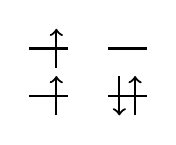
\begin{tikzpicture}[baseline={(current bounding box.center)}]
    % oberste MOs:
    \draw[thick] (0,0) -- (0.5,0); % erster Strich
    \draw[thick] (1,0) -- (1.5,0); % zweiter Strich
    % unterste MOs:
    \draw[thick] (0,-0.6) -- (0.5,-0.6); % dritter Strich
    \draw[thick] (1,-0.6) -- (1.5,-0.6); % vierter Strich
\draw[->, thick] (0.35, -0.25) -- (0.35, 0.25); 
\draw[-> , thick] (0.35, -0.85) -- (0.35, -0.35); 
 \draw[-> , thick] (1.35, -0.85) -- (1.35, -0.35); 
\draw[<- , thick] (1.15, -0.85) -- (1.15, -0.35); 
\end{tikzpicture}\qquad 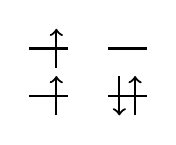
\begin{tikzpicture}[baseline={(current bounding box.center)}]
    % oberste MOs:
    \draw[thick] (0,0) -- (0.5,0); % erster Strich
    \draw[thick] (1,0) -- (1.5,0); % zweiter Strich
    % unterste MOs:
    \draw[thick] (0,-0.6) -- (0.5,-0.6); % dritter Strich
    \draw[thick] (1,-0.6) -- (1.5,-0.6); % vierter Strich
\draw[->, thick] (0.35, -0.25) -- (0.35, 0.25); 
\draw[-> , thick] (0.35, -0.85) -- (0.35, -0.35); 
 \draw[-> , thick] (1.35, -0.85) -- (1.35, -0.35); 
\draw[<- , thick] (1.15, -0.85) -- (1.15, -0.35); 
\end{tikzpicture}}\right)+\left(\text{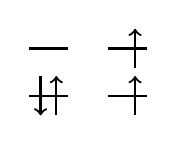
\begin{tikzpicture}[baseline={(current bounding box.center)}]
    % oberste MOs:
    \draw[thick] (0,0) -- (0.5,0); % erster Strich
    \draw[thick] (1,0) -- (1.5,0); % zweiter Strich
    % unterste MOs:
    \draw[thick] (0,-0.6) -- (0.5,-0.6); % dritter Strich
    \draw[thick] (1,-0.6) -- (1.5,-0.6); % vierter Strich
\draw[->, thick] (1.35, -0.25) -- (1.35, 0.25); 
\draw[-> , thick] (0.35, -0.85) -- (0.35, -0.35); 
\draw[<- , thick] (0.15, -0.85) -- (0.15, -0.35); 
 \draw[-> , thick] (1.35, -0.85) -- (1.35, -0.35); 
\end{tikzpicture}\qquad 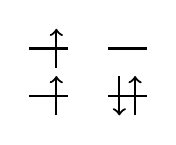
\begin{tikzpicture}[baseline={(current bounding box.center)}]
    % oberste MOs:
    \draw[thick] (0,0) -- (0.5,0); % erster Strich
    \draw[thick] (1,0) -- (1.5,0); % zweiter Strich
    % unterste MOs:
    \draw[thick] (0,-0.6) -- (0.5,-0.6); % dritter Strich
    \draw[thick] (1,-0.6) -- (1.5,-0.6); % vierter Strich
\draw[->, thick] (0.35, -0.25) -- (0.35, 0.25); 
\draw[-> , thick] (0.35, -0.85) -- (0.35, -0.35); 
 \draw[-> , thick] (1.35, -0.85) -- (1.35, -0.35); 
\draw[<- , thick] (1.15, -0.85) -- (1.15, -0.35); 
\end{tikzpicture}}\right)+\left(\text{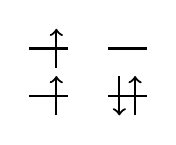
\begin{tikzpicture}[baseline={(current bounding box.center)}]
    % oberste MOs:
    \draw[thick] (0,0) -- (0.5,0); % erster Strich
    \draw[thick] (1,0) -- (1.5,0); % zweiter Strich
    % unterste MOs:
    \draw[thick] (0,-0.6) -- (0.5,-0.6); % dritter Strich
    \draw[thick] (1,-0.6) -- (1.5,-0.6); % vierter Strich
\draw[->, thick] (0.35, -0.25) -- (0.35, 0.25); 
\draw[-> , thick] (0.35, -0.85) -- (0.35, -0.35); 
 \draw[-> , thick] (1.35, -0.85) -- (1.35, -0.35); 
\draw[<- , thick] (1.15, -0.85) -- (1.15, -0.35); 
\end{tikzpicture}\qquad 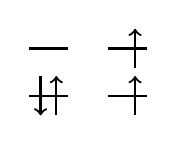
\begin{tikzpicture}[baseline={(current bounding box.center)}]
    % oberste MOs:
    \draw[thick] (0,0) -- (0.5,0); % erster Strich
    \draw[thick] (1,0) -- (1.5,0); % zweiter Strich
    % unterste MOs:
    \draw[thick] (0,-0.6) -- (0.5,-0.6); % dritter Strich
    \draw[thick] (1,-0.6) -- (1.5,-0.6); % vierter Strich
\draw[->, thick] (1.35, -0.25) -- (1.35, 0.25); 
\draw[-> , thick] (0.35, -0.85) -- (0.35, -0.35); 
\draw[<- , thick] (0.15, -0.85) -- (0.15, -0.35); 
 \draw[-> , thick] (1.35, -0.85) -- (1.35, -0.35); 
\end{tikzpicture}}\right)+\left(\text{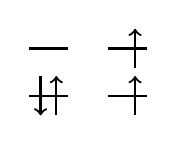
\begin{tikzpicture}[baseline={(current bounding box.center)}]
    % oberste MOs:
    \draw[thick] (0,0) -- (0.5,0); % erster Strich
    \draw[thick] (1,0) -- (1.5,0); % zweiter Strich
    % unterste MOs:
    \draw[thick] (0,-0.6) -- (0.5,-0.6); % dritter Strich
    \draw[thick] (1,-0.6) -- (1.5,-0.6); % vierter Strich
\draw[->, thick] (1.35, -0.25) -- (1.35, 0.25); 
\draw[-> , thick] (0.35, -0.85) -- (0.35, -0.35); 
\draw[<- , thick] (0.15, -0.85) -- (0.15, -0.35); 
 \draw[-> , thick] (1.35, -0.85) -- (1.35, -0.35); 
\end{tikzpicture}\qquad 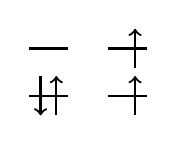
\begin{tikzpicture}[baseline={(current bounding box.center)}]
    % oberste MOs:
    \draw[thick] (0,0) -- (0.5,0); % erster Strich
    \draw[thick] (1,0) -- (1.5,0); % zweiter Strich
    % unterste MOs:
    \draw[thick] (0,-0.6) -- (0.5,-0.6); % dritter Strich
    \draw[thick] (1,-0.6) -- (1.5,-0.6); % vierter Strich
\draw[->, thick] (1.35, -0.25) -- (1.35, 0.25); 
\draw[-> , thick] (0.35, -0.85) -- (0.35, -0.35); 
\draw[<- , thick] (0.15, -0.85) -- (0.15, -0.35); 
 \draw[-> , thick] (1.35, -0.85) -- (1.35, -0.35); 
\end{tikzpicture}}\right)\\\\\]


bzw. in CI-Vektoren geschrieben: 
 $$+ 1 \cdot \left|aa20 \right| \cdot \left| aa20 \right| 
+ 1 \cdot \left|02aa \right| \cdot \left| aa20 \right| 
+ 1 \cdot \left|aa20 \right| \cdot \left| 02aa \right| 
+ 1 \cdot \left|02aa \right| \cdot \left| 02aa \right| 
$$



 bildet folgende mögliche Dimerkombinationen:

$$+ 1 \cdot \left|aa20aa20 \right| + 1 \cdot \left|02aa02aa \right| + \frac{1}{8} \cdot \left|02aaaa20 \right| + \frac{1}{8} \cdot \left|02a0aa2a \right| + \frac{1}{8} \cdot \left|022aaaa0 \right| + \frac{1}{8} \cdot \left|0220aaaa \right|  $$ $$ + \frac{1}{8} \cdot \left|0aaaa220 \right| + \frac{1}{8} \cdot \left|0aa0a22a \right| + \frac{1}{8} \cdot \left|0a2aa2a0 \right| + \frac{1}{8} \cdot \left|0a20a2aa \right| + \frac{1}{8} \cdot \left|a2aa0a20 \right| + \frac{1}{8} \cdot \left|a2a00a2a \right|  $$ $$ + \frac{1}{8} \cdot \left|a22a0aa0 \right| + \frac{1}{8} \cdot \left|a2200aaa \right| + \frac{1}{8} \cdot \left|aaaa0220 \right| + \frac{1}{8} \cdot \left|aaa0022a \right| + \frac{1}{8} \cdot \left|aa2a02a0 \right| + \frac{1}{8} \cdot \left|aa2002aa \right| $$



\end{minipage}
\vspace{0.5cm}
\hrule
\vspace{0.5cm}



\begin{minipage}{\linewidth}
$e^3 b_{2u}$ * $e^3 b_{3u}$ \quad = \quad $2.3$ * $1.2$
\[ +\left(\text{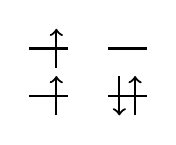
\begin{tikzpicture}[baseline={(current bounding box.center)}]
    % oberste MOs:
    \draw[thick] (0,0) -- (0.5,0); % erster Strich
    \draw[thick] (1,0) -- (1.5,0); % zweiter Strich
    % unterste MOs:
    \draw[thick] (0,-0.6) -- (0.5,-0.6); % dritter Strich
    \draw[thick] (1,-0.6) -- (1.5,-0.6); % vierter Strich
\draw[->, thick] (0.35, -0.25) -- (0.35, 0.25); 
\draw[-> , thick] (0.35, -0.85) -- (0.35, -0.35); 
 \draw[-> , thick] (1.35, -0.85) -- (1.35, -0.35); 
\draw[<- , thick] (1.15, -0.85) -- (1.15, -0.35); 
\end{tikzpicture}\qquad 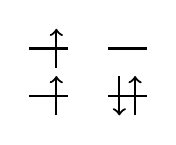
\begin{tikzpicture}[baseline={(current bounding box.center)}]
    % oberste MOs:
    \draw[thick] (0,0) -- (0.5,0); % erster Strich
    \draw[thick] (1,0) -- (1.5,0); % zweiter Strich
    % unterste MOs:
    \draw[thick] (0,-0.6) -- (0.5,-0.6); % dritter Strich
    \draw[thick] (1,-0.6) -- (1.5,-0.6); % vierter Strich
\draw[->, thick] (0.35, -0.25) -- (0.35, 0.25); 
\draw[-> , thick] (0.35, -0.85) -- (0.35, -0.35); 
 \draw[-> , thick] (1.35, -0.85) -- (1.35, -0.35); 
\draw[<- , thick] (1.15, -0.85) -- (1.15, -0.35); 
\end{tikzpicture}}\right)+\left(\text{\begin{tikzpicture}[baseline={(current bounding box.center)}]
    % oberste MOs:
    \draw[thick] (0,0) -- (0.5,0); % erster Strich
    \draw[thick] (1,0) -- (1.5,0); % zweiter Strich
    % unterste MOs:
    \draw[thick] (0,-0.6) -- (0.5,-0.6); % dritter Strich
    \draw[thick] (1,-0.6) -- (1.5,-0.6); % vierter Strich
\draw[->, thick] (1.35, -0.25) -- (1.35, 0.25); 
\draw[-> , thick] (0.35, -0.85) -- (0.35, -0.35); 
\draw[<- , thick] (0.15, -0.85) -- (0.15, -0.35); 
 \draw[-> , thick] (1.35, -0.85) -- (1.35, -0.35); 
\end{tikzpicture}\qquad \begin{tikzpicture}[baseline={(current bounding box.center)}]
    % oberste MOs:
    \draw[thick] (0,0) -- (0.5,0); % erster Strich
    \draw[thick] (1,0) -- (1.5,0); % zweiter Strich
    % unterste MOs:
    \draw[thick] (0,-0.6) -- (0.5,-0.6); % dritter Strich
    \draw[thick] (1,-0.6) -- (1.5,-0.6); % vierter Strich
\draw[->, thick] (0.35, -0.25) -- (0.35, 0.25); 
\draw[-> , thick] (0.35, -0.85) -- (0.35, -0.35); 
 \draw[-> , thick] (1.35, -0.85) -- (1.35, -0.35); 
\draw[<- , thick] (1.15, -0.85) -- (1.15, -0.35); 
\end{tikzpicture}}\right)-\left(\text{\begin{tikzpicture}[baseline={(current bounding box.center)}]
    % oberste MOs:
    \draw[thick] (0,0) -- (0.5,0); % erster Strich
    \draw[thick] (1,0) -- (1.5,0); % zweiter Strich
    % unterste MOs:
    \draw[thick] (0,-0.6) -- (0.5,-0.6); % dritter Strich
    \draw[thick] (1,-0.6) -- (1.5,-0.6); % vierter Strich
\draw[->, thick] (0.35, -0.25) -- (0.35, 0.25); 
\draw[-> , thick] (0.35, -0.85) -- (0.35, -0.35); 
 \draw[-> , thick] (1.35, -0.85) -- (1.35, -0.35); 
\draw[<- , thick] (1.15, -0.85) -- (1.15, -0.35); 
\end{tikzpicture}\qquad \begin{tikzpicture}[baseline={(current bounding box.center)}]
    % oberste MOs:
    \draw[thick] (0,0) -- (0.5,0); % erster Strich
    \draw[thick] (1,0) -- (1.5,0); % zweiter Strich
    % unterste MOs:
    \draw[thick] (0,-0.6) -- (0.5,-0.6); % dritter Strich
    \draw[thick] (1,-0.6) -- (1.5,-0.6); % vierter Strich
\draw[->, thick] (1.35, -0.25) -- (1.35, 0.25); 
\draw[-> , thick] (0.35, -0.85) -- (0.35, -0.35); 
\draw[<- , thick] (0.15, -0.85) -- (0.15, -0.35); 
 \draw[-> , thick] (1.35, -0.85) -- (1.35, -0.35); 
\end{tikzpicture}}\right)-\left(\text{\begin{tikzpicture}[baseline={(current bounding box.center)}]
    % oberste MOs:
    \draw[thick] (0,0) -- (0.5,0); % erster Strich
    \draw[thick] (1,0) -- (1.5,0); % zweiter Strich
    % unterste MOs:
    \draw[thick] (0,-0.6) -- (0.5,-0.6); % dritter Strich
    \draw[thick] (1,-0.6) -- (1.5,-0.6); % vierter Strich
\draw[->, thick] (1.35, -0.25) -- (1.35, 0.25); 
\draw[-> , thick] (0.35, -0.85) -- (0.35, -0.35); 
\draw[<- , thick] (0.15, -0.85) -- (0.15, -0.35); 
 \draw[-> , thick] (1.35, -0.85) -- (1.35, -0.35); 
\end{tikzpicture}\qquad \begin{tikzpicture}[baseline={(current bounding box.center)}]
    % oberste MOs:
    \draw[thick] (0,0) -- (0.5,0); % erster Strich
    \draw[thick] (1,0) -- (1.5,0); % zweiter Strich
    % unterste MOs:
    \draw[thick] (0,-0.6) -- (0.5,-0.6); % dritter Strich
    \draw[thick] (1,-0.6) -- (1.5,-0.6); % vierter Strich
\draw[->, thick] (1.35, -0.25) -- (1.35, 0.25); 
\draw[-> , thick] (0.35, -0.85) -- (0.35, -0.35); 
\draw[<- , thick] (0.15, -0.85) -- (0.15, -0.35); 
 \draw[-> , thick] (1.35, -0.85) -- (1.35, -0.35); 
\end{tikzpicture}}\right)\\\\\]


bzw. in CI-Vektoren geschrieben: 
 $$+ 1 \cdot \left|aa20 \right| \cdot \left| aa20 \right| 
+ 1 \cdot \left|02aa \right| \cdot \left| aa20 \right| 
- 1 \cdot \left|aa20 \right| \cdot \left| 02aa \right| 
- 1 \cdot \left|02aa \right| \cdot \left| 02aa \right| 
$$



 bildet folgende mögliche Dimerkombinationen:

$$+ 1 \cdot \left|aa20aa20 \right| - 1 \cdot \left|02aa02aa \right| $$



\end{minipage}
\vspace{0.5cm}
\hrule
\vspace{0.5cm}



\begin{minipage}{\linewidth}
$e^3 b_{2u}$ * $i^3 b_{3u}$ \quad = \quad $2.3$ * $2.2$
\[ +\left(\text{\begin{tikzpicture}[baseline={(current bounding box.center)}]
    % oberste MOs:
    \draw[thick] (0,0) -- (0.5,0); % erster Strich
    \draw[thick] (1,0) -- (1.5,0); % zweiter Strich
    % unterste MOs:
    \draw[thick] (0,-0.6) -- (0.5,-0.6); % dritter Strich
    \draw[thick] (1,-0.6) -- (1.5,-0.6); % vierter Strich
\draw[->, thick] (0.35, -0.25) -- (0.35, 0.25); 
\draw[-> , thick] (0.35, -0.85) -- (0.35, -0.35); 
 \draw[-> , thick] (1.35, -0.85) -- (1.35, -0.35); 
\draw[<- , thick] (1.15, -0.85) -- (1.15, -0.35); 
\end{tikzpicture}\qquad \begin{tikzpicture}[baseline={(current bounding box.center)}]
    % oberste MOs:
    \draw[thick] (0,0) -- (0.5,0); % erster Strich
    \draw[thick] (1,0) -- (1.5,0); % zweiter Strich
    % unterste MOs:
    \draw[thick] (0,-0.6) -- (0.5,-0.6); % dritter Strich
    \draw[thick] (1,-0.6) -- (1.5,-0.6); % vierter Strich
\draw[->, thick] (0.35, -0.25) -- (0.35, 0.25); 
\draw[-> , thick] (0.35, -0.85) -- (0.35, -0.35); 
 \draw[-> , thick] (1.35, -0.85) -- (1.35, -0.35); 
\draw[<- , thick] (1.15, -0.85) -- (1.15, -0.35); 
\end{tikzpicture}}\right)+\left(\text{\begin{tikzpicture}[baseline={(current bounding box.center)}]
    % oberste MOs:
    \draw[thick] (0,0) -- (0.5,0); % erster Strich
    \draw[thick] (1,0) -- (1.5,0); % zweiter Strich
    % unterste MOs:
    \draw[thick] (0,-0.6) -- (0.5,-0.6); % dritter Strich
    \draw[thick] (1,-0.6) -- (1.5,-0.6); % vierter Strich
\draw[->, thick] (1.35, -0.25) -- (1.35, 0.25); 
\draw[-> , thick] (0.35, -0.85) -- (0.35, -0.35); 
\draw[<- , thick] (0.15, -0.85) -- (0.15, -0.35); 
 \draw[-> , thick] (1.35, -0.85) -- (1.35, -0.35); 
\end{tikzpicture}\qquad \begin{tikzpicture}[baseline={(current bounding box.center)}]
    % oberste MOs:
    \draw[thick] (0,0) -- (0.5,0); % erster Strich
    \draw[thick] (1,0) -- (1.5,0); % zweiter Strich
    % unterste MOs:
    \draw[thick] (0,-0.6) -- (0.5,-0.6); % dritter Strich
    \draw[thick] (1,-0.6) -- (1.5,-0.6); % vierter Strich
\draw[->, thick] (0.35, -0.25) -- (0.35, 0.25); 
\draw[-> , thick] (0.35, -0.85) -- (0.35, -0.35); 
 \draw[-> , thick] (1.35, -0.85) -- (1.35, -0.35); 
\draw[<- , thick] (1.15, -0.85) -- (1.15, -0.35); 
\end{tikzpicture}}\right)+\left(\text{\begin{tikzpicture}[baseline={(current bounding box.center)}]
    % oberste MOs:
    \draw[thick] (0,0) -- (0.5,0); % erster Strich
    \draw[thick] (1,0) -- (1.5,0); % zweiter Strich
    % unterste MOs:
    \draw[thick] (0,-0.6) -- (0.5,-0.6); % dritter Strich
    \draw[thick] (1,-0.6) -- (1.5,-0.6); % vierter Strich
\draw[->, thick] (0.35, -0.25) -- (0.35, 0.25); 
\draw[-> , thick] (0.35, -0.85) -- (0.35, -0.35); 
 \draw[-> , thick] (1.35, -0.85) -- (1.35, -0.35); 
\draw[<- , thick] (1.15, -0.85) -- (1.15, -0.35); 
\end{tikzpicture}\qquad \begin{tikzpicture}[baseline={(current bounding box.center)}]
    % oberste MOs:
    \draw[thick] (0,0) -- (0.5,0); % erster Strich
    \draw[thick] (1,0) -- (1.5,0); % zweiter Strich
    % unterste MOs:
    \draw[thick] (0,-0.6) -- (0.5,-0.6); % dritter Strich
    \draw[thick] (1,-0.6) -- (1.5,-0.6); % vierter Strich
\draw[->, thick] (1.35, -0.25) -- (1.35, 0.25); 
\draw[-> , thick] (0.35, -0.85) -- (0.35, -0.35); 
\draw[<- , thick] (0.15, -0.85) -- (0.15, -0.35); 
 \draw[-> , thick] (1.35, -0.85) -- (1.35, -0.35); 
\end{tikzpicture}}\right)+\left(\text{\begin{tikzpicture}[baseline={(current bounding box.center)}]
    % oberste MOs:
    \draw[thick] (0,0) -- (0.5,0); % erster Strich
    \draw[thick] (1,0) -- (1.5,0); % zweiter Strich
    % unterste MOs:
    \draw[thick] (0,-0.6) -- (0.5,-0.6); % dritter Strich
    \draw[thick] (1,-0.6) -- (1.5,-0.6); % vierter Strich
\draw[->, thick] (1.35, -0.25) -- (1.35, 0.25); 
\draw[-> , thick] (0.35, -0.85) -- (0.35, -0.35); 
\draw[<- , thick] (0.15, -0.85) -- (0.15, -0.35); 
 \draw[-> , thick] (1.35, -0.85) -- (1.35, -0.35); 
\end{tikzpicture}\qquad \begin{tikzpicture}[baseline={(current bounding box.center)}]
    % oberste MOs:
    \draw[thick] (0,0) -- (0.5,0); % erster Strich
    \draw[thick] (1,0) -- (1.5,0); % zweiter Strich
    % unterste MOs:
    \draw[thick] (0,-0.6) -- (0.5,-0.6); % dritter Strich
    \draw[thick] (1,-0.6) -- (1.5,-0.6); % vierter Strich
\draw[->, thick] (1.35, -0.25) -- (1.35, 0.25); 
\draw[-> , thick] (0.35, -0.85) -- (0.35, -0.35); 
\draw[<- , thick] (0.15, -0.85) -- (0.15, -0.35); 
 \draw[-> , thick] (1.35, -0.85) -- (1.35, -0.35); 
\end{tikzpicture}}\right)\\\\\]


bzw. in CI-Vektoren geschrieben: 
 $$+ 1 \cdot \left|aa20 \right| \cdot \left| aa20 \right| 
+ 1 \cdot \left|02aa \right| \cdot \left| aa20 \right| 
+ 1 \cdot \left|aa20 \right| \cdot \left| 02aa \right| 
+ 1 \cdot \left|02aa \right| \cdot \left| 02aa \right| 
$$



 bildet folgende mögliche Dimerkombinationen:

$$+ 1 \cdot \left|aa20aa20 \right| + 1 \cdot \left|02aa02aa \right| + \frac{1}{8} \cdot \left|02aaaa20 \right| + \frac{1}{8} \cdot \left|02a0aa2a \right| + \frac{1}{8} \cdot \left|022aaaa0 \right| + \frac{1}{8} \cdot \left|0220aaaa \right|  $$ $$ + \frac{1}{8} \cdot \left|0aaaa220 \right| + \frac{1}{8} \cdot \left|0aa0a22a \right| + \frac{1}{8} \cdot \left|0a2aa2a0 \right| + \frac{1}{8} \cdot \left|0a20a2aa \right| + \frac{1}{8} \cdot \left|a2aa0a20 \right| + \frac{1}{8} \cdot \left|a2a00a2a \right|  $$ $$ + \frac{1}{8} \cdot \left|a22a0aa0 \right| + \frac{1}{8} \cdot \left|a2200aaa \right| + \frac{1}{8} \cdot \left|aaaa0220 \right| + \frac{1}{8} \cdot \left|aaa0022a \right| + \frac{1}{8} \cdot \left|aa2a02a0 \right| + \frac{1}{8} \cdot \left|aa2002aa \right| $$



\end{minipage}
\vspace{0.5cm}
\hrule
\vspace{0.5cm}



\begin{minipage}{\linewidth}
$e^3 b_{3u}$ * $i^3 b_{2u}$ \quad = \quad $1.2$ * $1.3$
\[ +\left(\text{\begin{tikzpicture}[baseline={(current bounding box.center)}]
    % oberste MOs:
    \draw[thick] (0,0) -- (0.5,0); % erster Strich
    \draw[thick] (1,0) -- (1.5,0); % zweiter Strich
    % unterste MOs:
    \draw[thick] (0,-0.6) -- (0.5,-0.6); % dritter Strich
    \draw[thick] (1,-0.6) -- (1.5,-0.6); % vierter Strich
\draw[->, thick] (0.35, -0.25) -- (0.35, 0.25); 
\draw[-> , thick] (0.35, -0.85) -- (0.35, -0.35); 
 \draw[-> , thick] (1.35, -0.85) -- (1.35, -0.35); 
\draw[<- , thick] (1.15, -0.85) -- (1.15, -0.35); 
\end{tikzpicture}\qquad \begin{tikzpicture}[baseline={(current bounding box.center)}]
    % oberste MOs:
    \draw[thick] (0,0) -- (0.5,0); % erster Strich
    \draw[thick] (1,0) -- (1.5,0); % zweiter Strich
    % unterste MOs:
    \draw[thick] (0,-0.6) -- (0.5,-0.6); % dritter Strich
    \draw[thick] (1,-0.6) -- (1.5,-0.6); % vierter Strich
\draw[->, thick] (0.35, -0.25) -- (0.35, 0.25); 
\draw[-> , thick] (0.35, -0.85) -- (0.35, -0.35); 
 \draw[-> , thick] (1.35, -0.85) -- (1.35, -0.35); 
\draw[<- , thick] (1.15, -0.85) -- (1.15, -0.35); 
\end{tikzpicture}}\right)-\left(\text{\begin{tikzpicture}[baseline={(current bounding box.center)}]
    % oberste MOs:
    \draw[thick] (0,0) -- (0.5,0); % erster Strich
    \draw[thick] (1,0) -- (1.5,0); % zweiter Strich
    % unterste MOs:
    \draw[thick] (0,-0.6) -- (0.5,-0.6); % dritter Strich
    \draw[thick] (1,-0.6) -- (1.5,-0.6); % vierter Strich
\draw[->, thick] (1.35, -0.25) -- (1.35, 0.25); 
\draw[-> , thick] (0.35, -0.85) -- (0.35, -0.35); 
\draw[<- , thick] (0.15, -0.85) -- (0.15, -0.35); 
 \draw[-> , thick] (1.35, -0.85) -- (1.35, -0.35); 
\end{tikzpicture}\qquad \begin{tikzpicture}[baseline={(current bounding box.center)}]
    % oberste MOs:
    \draw[thick] (0,0) -- (0.5,0); % erster Strich
    \draw[thick] (1,0) -- (1.5,0); % zweiter Strich
    % unterste MOs:
    \draw[thick] (0,-0.6) -- (0.5,-0.6); % dritter Strich
    \draw[thick] (1,-0.6) -- (1.5,-0.6); % vierter Strich
\draw[->, thick] (0.35, -0.25) -- (0.35, 0.25); 
\draw[-> , thick] (0.35, -0.85) -- (0.35, -0.35); 
 \draw[-> , thick] (1.35, -0.85) -- (1.35, -0.35); 
\draw[<- , thick] (1.15, -0.85) -- (1.15, -0.35); 
\end{tikzpicture}}\right)-\left(\text{\begin{tikzpicture}[baseline={(current bounding box.center)}]
    % oberste MOs:
    \draw[thick] (0,0) -- (0.5,0); % erster Strich
    \draw[thick] (1,0) -- (1.5,0); % zweiter Strich
    % unterste MOs:
    \draw[thick] (0,-0.6) -- (0.5,-0.6); % dritter Strich
    \draw[thick] (1,-0.6) -- (1.5,-0.6); % vierter Strich
\draw[->, thick] (0.35, -0.25) -- (0.35, 0.25); 
\draw[-> , thick] (0.35, -0.85) -- (0.35, -0.35); 
 \draw[-> , thick] (1.35, -0.85) -- (1.35, -0.35); 
\draw[<- , thick] (1.15, -0.85) -- (1.15, -0.35); 
\end{tikzpicture}\qquad \begin{tikzpicture}[baseline={(current bounding box.center)}]
    % oberste MOs:
    \draw[thick] (0,0) -- (0.5,0); % erster Strich
    \draw[thick] (1,0) -- (1.5,0); % zweiter Strich
    % unterste MOs:
    \draw[thick] (0,-0.6) -- (0.5,-0.6); % dritter Strich
    \draw[thick] (1,-0.6) -- (1.5,-0.6); % vierter Strich
\draw[->, thick] (1.35, -0.25) -- (1.35, 0.25); 
\draw[-> , thick] (0.35, -0.85) -- (0.35, -0.35); 
\draw[<- , thick] (0.15, -0.85) -- (0.15, -0.35); 
 \draw[-> , thick] (1.35, -0.85) -- (1.35, -0.35); 
\end{tikzpicture}}\right)+\left(\text{\begin{tikzpicture}[baseline={(current bounding box.center)}]
    % oberste MOs:
    \draw[thick] (0,0) -- (0.5,0); % erster Strich
    \draw[thick] (1,0) -- (1.5,0); % zweiter Strich
    % unterste MOs:
    \draw[thick] (0,-0.6) -- (0.5,-0.6); % dritter Strich
    \draw[thick] (1,-0.6) -- (1.5,-0.6); % vierter Strich
\draw[->, thick] (1.35, -0.25) -- (1.35, 0.25); 
\draw[-> , thick] (0.35, -0.85) -- (0.35, -0.35); 
\draw[<- , thick] (0.15, -0.85) -- (0.15, -0.35); 
 \draw[-> , thick] (1.35, -0.85) -- (1.35, -0.35); 
\end{tikzpicture}\qquad \begin{tikzpicture}[baseline={(current bounding box.center)}]
    % oberste MOs:
    \draw[thick] (0,0) -- (0.5,0); % erster Strich
    \draw[thick] (1,0) -- (1.5,0); % zweiter Strich
    % unterste MOs:
    \draw[thick] (0,-0.6) -- (0.5,-0.6); % dritter Strich
    \draw[thick] (1,-0.6) -- (1.5,-0.6); % vierter Strich
\draw[->, thick] (1.35, -0.25) -- (1.35, 0.25); 
\draw[-> , thick] (0.35, -0.85) -- (0.35, -0.35); 
\draw[<- , thick] (0.15, -0.85) -- (0.15, -0.35); 
 \draw[-> , thick] (1.35, -0.85) -- (1.35, -0.35); 
\end{tikzpicture}}\right)\\\\\]


bzw. in CI-Vektoren geschrieben: 
 $$+ 1 \cdot \left|aa20 \right| \cdot \left| aa20 \right| 
- 1 \cdot \left|02aa \right| \cdot \left| aa20 \right| 
- 1 \cdot \left|aa20 \right| \cdot \left| 02aa \right| 
+ 1 \cdot \left|02aa \right| \cdot \left| 02aa \right| 
$$



 bildet folgende mögliche Dimerkombinationen:

$$+ 1 \cdot \left|aa20aa20 \right| + 1 \cdot \left|02aa02aa \right| - \frac{1}{8} \cdot \left|02aaaa20 \right| - \frac{1}{8} \cdot \left|02a0aa2a \right| - \frac{1}{8} \cdot \left|022aaaa0 \right| - \frac{1}{8} \cdot \left|0220aaaa \right|  $$ $$ - \frac{1}{8} \cdot \left|0aaaa220 \right| - \frac{1}{8} \cdot \left|0aa0a22a \right| - \frac{1}{8} \cdot \left|0a2aa2a0 \right| - \frac{1}{8} \cdot \left|0a20a2aa \right| - \frac{1}{8} \cdot \left|a2aa0a20 \right| - \frac{1}{8} \cdot \left|a2a00a2a \right|  $$ $$ - \frac{1}{8} \cdot \left|a22a0aa0 \right| - \frac{1}{8} \cdot \left|a2200aaa \right| - \frac{1}{8} \cdot \left|aaaa0220 \right| - \frac{1}{8} \cdot \left|aaa0022a \right| - \frac{1}{8} \cdot \left|aa2a02a0 \right| - \frac{1}{8} \cdot \left|aa2002aa \right| $$



\end{minipage}
\vspace{0.5cm}
\hrule
\vspace{0.5cm}



\begin{minipage}{\linewidth}
$e^3 b_{3u}$ * $e^3 b_{2u}$ \quad = \quad $1.2$ * $2.3$
\[ +\left(\text{\begin{tikzpicture}[baseline={(current bounding box.center)}]
    % oberste MOs:
    \draw[thick] (0,0) -- (0.5,0); % erster Strich
    \draw[thick] (1,0) -- (1.5,0); % zweiter Strich
    % unterste MOs:
    \draw[thick] (0,-0.6) -- (0.5,-0.6); % dritter Strich
    \draw[thick] (1,-0.6) -- (1.5,-0.6); % vierter Strich
\draw[->, thick] (0.35, -0.25) -- (0.35, 0.25); 
\draw[-> , thick] (0.35, -0.85) -- (0.35, -0.35); 
 \draw[-> , thick] (1.35, -0.85) -- (1.35, -0.35); 
\draw[<- , thick] (1.15, -0.85) -- (1.15, -0.35); 
\end{tikzpicture}\qquad \begin{tikzpicture}[baseline={(current bounding box.center)}]
    % oberste MOs:
    \draw[thick] (0,0) -- (0.5,0); % erster Strich
    \draw[thick] (1,0) -- (1.5,0); % zweiter Strich
    % unterste MOs:
    \draw[thick] (0,-0.6) -- (0.5,-0.6); % dritter Strich
    \draw[thick] (1,-0.6) -- (1.5,-0.6); % vierter Strich
\draw[->, thick] (0.35, -0.25) -- (0.35, 0.25); 
\draw[-> , thick] (0.35, -0.85) -- (0.35, -0.35); 
 \draw[-> , thick] (1.35, -0.85) -- (1.35, -0.35); 
\draw[<- , thick] (1.15, -0.85) -- (1.15, -0.35); 
\end{tikzpicture}}\right)-\left(\text{\begin{tikzpicture}[baseline={(current bounding box.center)}]
    % oberste MOs:
    \draw[thick] (0,0) -- (0.5,0); % erster Strich
    \draw[thick] (1,0) -- (1.5,0); % zweiter Strich
    % unterste MOs:
    \draw[thick] (0,-0.6) -- (0.5,-0.6); % dritter Strich
    \draw[thick] (1,-0.6) -- (1.5,-0.6); % vierter Strich
\draw[->, thick] (1.35, -0.25) -- (1.35, 0.25); 
\draw[-> , thick] (0.35, -0.85) -- (0.35, -0.35); 
\draw[<- , thick] (0.15, -0.85) -- (0.15, -0.35); 
 \draw[-> , thick] (1.35, -0.85) -- (1.35, -0.35); 
\end{tikzpicture}\qquad \begin{tikzpicture}[baseline={(current bounding box.center)}]
    % oberste MOs:
    \draw[thick] (0,0) -- (0.5,0); % erster Strich
    \draw[thick] (1,0) -- (1.5,0); % zweiter Strich
    % unterste MOs:
    \draw[thick] (0,-0.6) -- (0.5,-0.6); % dritter Strich
    \draw[thick] (1,-0.6) -- (1.5,-0.6); % vierter Strich
\draw[->, thick] (0.35, -0.25) -- (0.35, 0.25); 
\draw[-> , thick] (0.35, -0.85) -- (0.35, -0.35); 
 \draw[-> , thick] (1.35, -0.85) -- (1.35, -0.35); 
\draw[<- , thick] (1.15, -0.85) -- (1.15, -0.35); 
\end{tikzpicture}}\right)+\left(\text{\begin{tikzpicture}[baseline={(current bounding box.center)}]
    % oberste MOs:
    \draw[thick] (0,0) -- (0.5,0); % erster Strich
    \draw[thick] (1,0) -- (1.5,0); % zweiter Strich
    % unterste MOs:
    \draw[thick] (0,-0.6) -- (0.5,-0.6); % dritter Strich
    \draw[thick] (1,-0.6) -- (1.5,-0.6); % vierter Strich
\draw[->, thick] (0.35, -0.25) -- (0.35, 0.25); 
\draw[-> , thick] (0.35, -0.85) -- (0.35, -0.35); 
 \draw[-> , thick] (1.35, -0.85) -- (1.35, -0.35); 
\draw[<- , thick] (1.15, -0.85) -- (1.15, -0.35); 
\end{tikzpicture}\qquad \begin{tikzpicture}[baseline={(current bounding box.center)}]
    % oberste MOs:
    \draw[thick] (0,0) -- (0.5,0); % erster Strich
    \draw[thick] (1,0) -- (1.5,0); % zweiter Strich
    % unterste MOs:
    \draw[thick] (0,-0.6) -- (0.5,-0.6); % dritter Strich
    \draw[thick] (1,-0.6) -- (1.5,-0.6); % vierter Strich
\draw[->, thick] (1.35, -0.25) -- (1.35, 0.25); 
\draw[-> , thick] (0.35, -0.85) -- (0.35, -0.35); 
\draw[<- , thick] (0.15, -0.85) -- (0.15, -0.35); 
 \draw[-> , thick] (1.35, -0.85) -- (1.35, -0.35); 
\end{tikzpicture}}\right)-\left(\text{\begin{tikzpicture}[baseline={(current bounding box.center)}]
    % oberste MOs:
    \draw[thick] (0,0) -- (0.5,0); % erster Strich
    \draw[thick] (1,0) -- (1.5,0); % zweiter Strich
    % unterste MOs:
    \draw[thick] (0,-0.6) -- (0.5,-0.6); % dritter Strich
    \draw[thick] (1,-0.6) -- (1.5,-0.6); % vierter Strich
\draw[->, thick] (1.35, -0.25) -- (1.35, 0.25); 
\draw[-> , thick] (0.35, -0.85) -- (0.35, -0.35); 
\draw[<- , thick] (0.15, -0.85) -- (0.15, -0.35); 
 \draw[-> , thick] (1.35, -0.85) -- (1.35, -0.35); 
\end{tikzpicture}\qquad \begin{tikzpicture}[baseline={(current bounding box.center)}]
    % oberste MOs:
    \draw[thick] (0,0) -- (0.5,0); % erster Strich
    \draw[thick] (1,0) -- (1.5,0); % zweiter Strich
    % unterste MOs:
    \draw[thick] (0,-0.6) -- (0.5,-0.6); % dritter Strich
    \draw[thick] (1,-0.6) -- (1.5,-0.6); % vierter Strich
\draw[->, thick] (1.35, -0.25) -- (1.35, 0.25); 
\draw[-> , thick] (0.35, -0.85) -- (0.35, -0.35); 
\draw[<- , thick] (0.15, -0.85) -- (0.15, -0.35); 
 \draw[-> , thick] (1.35, -0.85) -- (1.35, -0.35); 
\end{tikzpicture}}\right)\\\\\]


bzw. in CI-Vektoren geschrieben: 
 $$+ 1 \cdot \left|aa20 \right| \cdot \left| aa20 \right| 
- 1 \cdot \left|02aa \right| \cdot \left| aa20 \right| 
+ 1 \cdot \left|aa20 \right| \cdot \left| 02aa \right| 
- 1 \cdot \left|02aa \right| \cdot \left| 02aa \right| 
$$



 bildet folgende mögliche Dimerkombinationen:

$$+ 1 \cdot \left|aa20aa20 \right| - 1 \cdot \left|02aa02aa \right| $$



\end{minipage}
\vspace{0.5cm}
\hrule
\vspace{0.5cm}



\begin{minipage}{\linewidth}
$e^3 b_{3u}$ * $e^3 b_{3u}$ \quad = \quad $1.2$ * $1.2$
\[ +\left(\text{\begin{tikzpicture}[baseline={(current bounding box.center)}]
    % oberste MOs:
    \draw[thick] (0,0) -- (0.5,0); % erster Strich
    \draw[thick] (1,0) -- (1.5,0); % zweiter Strich
    % unterste MOs:
    \draw[thick] (0,-0.6) -- (0.5,-0.6); % dritter Strich
    \draw[thick] (1,-0.6) -- (1.5,-0.6); % vierter Strich
\draw[->, thick] (0.35, -0.25) -- (0.35, 0.25); 
\draw[-> , thick] (0.35, -0.85) -- (0.35, -0.35); 
 \draw[-> , thick] (1.35, -0.85) -- (1.35, -0.35); 
\draw[<- , thick] (1.15, -0.85) -- (1.15, -0.35); 
\end{tikzpicture}\qquad \begin{tikzpicture}[baseline={(current bounding box.center)}]
    % oberste MOs:
    \draw[thick] (0,0) -- (0.5,0); % erster Strich
    \draw[thick] (1,0) -- (1.5,0); % zweiter Strich
    % unterste MOs:
    \draw[thick] (0,-0.6) -- (0.5,-0.6); % dritter Strich
    \draw[thick] (1,-0.6) -- (1.5,-0.6); % vierter Strich
\draw[->, thick] (0.35, -0.25) -- (0.35, 0.25); 
\draw[-> , thick] (0.35, -0.85) -- (0.35, -0.35); 
 \draw[-> , thick] (1.35, -0.85) -- (1.35, -0.35); 
\draw[<- , thick] (1.15, -0.85) -- (1.15, -0.35); 
\end{tikzpicture}}\right)-\left(\text{\begin{tikzpicture}[baseline={(current bounding box.center)}]
    % oberste MOs:
    \draw[thick] (0,0) -- (0.5,0); % erster Strich
    \draw[thick] (1,0) -- (1.5,0); % zweiter Strich
    % unterste MOs:
    \draw[thick] (0,-0.6) -- (0.5,-0.6); % dritter Strich
    \draw[thick] (1,-0.6) -- (1.5,-0.6); % vierter Strich
\draw[->, thick] (1.35, -0.25) -- (1.35, 0.25); 
\draw[-> , thick] (0.35, -0.85) -- (0.35, -0.35); 
\draw[<- , thick] (0.15, -0.85) -- (0.15, -0.35); 
 \draw[-> , thick] (1.35, -0.85) -- (1.35, -0.35); 
\end{tikzpicture}\qquad \begin{tikzpicture}[baseline={(current bounding box.center)}]
    % oberste MOs:
    \draw[thick] (0,0) -- (0.5,0); % erster Strich
    \draw[thick] (1,0) -- (1.5,0); % zweiter Strich
    % unterste MOs:
    \draw[thick] (0,-0.6) -- (0.5,-0.6); % dritter Strich
    \draw[thick] (1,-0.6) -- (1.5,-0.6); % vierter Strich
\draw[->, thick] (0.35, -0.25) -- (0.35, 0.25); 
\draw[-> , thick] (0.35, -0.85) -- (0.35, -0.35); 
 \draw[-> , thick] (1.35, -0.85) -- (1.35, -0.35); 
\draw[<- , thick] (1.15, -0.85) -- (1.15, -0.35); 
\end{tikzpicture}}\right)-\left(\text{\begin{tikzpicture}[baseline={(current bounding box.center)}]
    % oberste MOs:
    \draw[thick] (0,0) -- (0.5,0); % erster Strich
    \draw[thick] (1,0) -- (1.5,0); % zweiter Strich
    % unterste MOs:
    \draw[thick] (0,-0.6) -- (0.5,-0.6); % dritter Strich
    \draw[thick] (1,-0.6) -- (1.5,-0.6); % vierter Strich
\draw[->, thick] (0.35, -0.25) -- (0.35, 0.25); 
\draw[-> , thick] (0.35, -0.85) -- (0.35, -0.35); 
 \draw[-> , thick] (1.35, -0.85) -- (1.35, -0.35); 
\draw[<- , thick] (1.15, -0.85) -- (1.15, -0.35); 
\end{tikzpicture}\qquad \begin{tikzpicture}[baseline={(current bounding box.center)}]
    % oberste MOs:
    \draw[thick] (0,0) -- (0.5,0); % erster Strich
    \draw[thick] (1,0) -- (1.5,0); % zweiter Strich
    % unterste MOs:
    \draw[thick] (0,-0.6) -- (0.5,-0.6); % dritter Strich
    \draw[thick] (1,-0.6) -- (1.5,-0.6); % vierter Strich
\draw[->, thick] (1.35, -0.25) -- (1.35, 0.25); 
\draw[-> , thick] (0.35, -0.85) -- (0.35, -0.35); 
\draw[<- , thick] (0.15, -0.85) -- (0.15, -0.35); 
 \draw[-> , thick] (1.35, -0.85) -- (1.35, -0.35); 
\end{tikzpicture}}\right)+\left(\text{\begin{tikzpicture}[baseline={(current bounding box.center)}]
    % oberste MOs:
    \draw[thick] (0,0) -- (0.5,0); % erster Strich
    \draw[thick] (1,0) -- (1.5,0); % zweiter Strich
    % unterste MOs:
    \draw[thick] (0,-0.6) -- (0.5,-0.6); % dritter Strich
    \draw[thick] (1,-0.6) -- (1.5,-0.6); % vierter Strich
\draw[->, thick] (1.35, -0.25) -- (1.35, 0.25); 
\draw[-> , thick] (0.35, -0.85) -- (0.35, -0.35); 
\draw[<- , thick] (0.15, -0.85) -- (0.15, -0.35); 
 \draw[-> , thick] (1.35, -0.85) -- (1.35, -0.35); 
\end{tikzpicture}\qquad \begin{tikzpicture}[baseline={(current bounding box.center)}]
    % oberste MOs:
    \draw[thick] (0,0) -- (0.5,0); % erster Strich
    \draw[thick] (1,0) -- (1.5,0); % zweiter Strich
    % unterste MOs:
    \draw[thick] (0,-0.6) -- (0.5,-0.6); % dritter Strich
    \draw[thick] (1,-0.6) -- (1.5,-0.6); % vierter Strich
\draw[->, thick] (1.35, -0.25) -- (1.35, 0.25); 
\draw[-> , thick] (0.35, -0.85) -- (0.35, -0.35); 
\draw[<- , thick] (0.15, -0.85) -- (0.15, -0.35); 
 \draw[-> , thick] (1.35, -0.85) -- (1.35, -0.35); 
\end{tikzpicture}}\right)\\\\\]


bzw. in CI-Vektoren geschrieben: 
 $$+ 1 \cdot \left|aa20 \right| \cdot \left| aa20 \right| 
- 1 \cdot \left|02aa \right| \cdot \left| aa20 \right| 
- 1 \cdot \left|aa20 \right| \cdot \left| 02aa \right| 
+ 1 \cdot \left|02aa \right| \cdot \left| 02aa \right| 
$$



 bildet folgende mögliche Dimerkombinationen:

$$+ 1 \cdot \left|aa20aa20 \right| + 1 \cdot \left|02aa02aa \right| - \frac{1}{8} \cdot \left|02aaaa20 \right| - \frac{1}{8} \cdot \left|02a0aa2a \right| - \frac{1}{8} \cdot \left|022aaaa0 \right| - \frac{1}{8} \cdot \left|0220aaaa \right|  $$ $$ - \frac{1}{8} \cdot \left|0aaaa220 \right| - \frac{1}{8} \cdot \left|0aa0a22a \right| - \frac{1}{8} \cdot \left|0a2aa2a0 \right| - \frac{1}{8} \cdot \left|0a20a2aa \right| - \frac{1}{8} \cdot \left|a2aa0a20 \right| - \frac{1}{8} \cdot \left|a2a00a2a \right|  $$ $$ - \frac{1}{8} \cdot \left|a22a0aa0 \right| - \frac{1}{8} \cdot \left|a2200aaa \right| - \frac{1}{8} \cdot \left|aaaa0220 \right| - \frac{1}{8} \cdot \left|aaa0022a \right| - \frac{1}{8} \cdot \left|aa2a02a0 \right| - \frac{1}{8} \cdot \left|aa2002aa \right| $$



\end{minipage}
\vspace{0.5cm}
\hrule
\vspace{0.5cm}



\begin{minipage}{\linewidth}
$e^3 b_{3u}$ * $i^3 b_{3u}$ \quad = \quad $1.2$ * $2.2$
\[ +\left(\text{\begin{tikzpicture}[baseline={(current bounding box.center)}]
    % oberste MOs:
    \draw[thick] (0,0) -- (0.5,0); % erster Strich
    \draw[thick] (1,0) -- (1.5,0); % zweiter Strich
    % unterste MOs:
    \draw[thick] (0,-0.6) -- (0.5,-0.6); % dritter Strich
    \draw[thick] (1,-0.6) -- (1.5,-0.6); % vierter Strich
\draw[->, thick] (0.35, -0.25) -- (0.35, 0.25); 
\draw[-> , thick] (0.35, -0.85) -- (0.35, -0.35); 
 \draw[-> , thick] (1.35, -0.85) -- (1.35, -0.35); 
\draw[<- , thick] (1.15, -0.85) -- (1.15, -0.35); 
\end{tikzpicture}\qquad \begin{tikzpicture}[baseline={(current bounding box.center)}]
    % oberste MOs:
    \draw[thick] (0,0) -- (0.5,0); % erster Strich
    \draw[thick] (1,0) -- (1.5,0); % zweiter Strich
    % unterste MOs:
    \draw[thick] (0,-0.6) -- (0.5,-0.6); % dritter Strich
    \draw[thick] (1,-0.6) -- (1.5,-0.6); % vierter Strich
\draw[->, thick] (0.35, -0.25) -- (0.35, 0.25); 
\draw[-> , thick] (0.35, -0.85) -- (0.35, -0.35); 
 \draw[-> , thick] (1.35, -0.85) -- (1.35, -0.35); 
\draw[<- , thick] (1.15, -0.85) -- (1.15, -0.35); 
\end{tikzpicture}}\right)-\left(\text{\begin{tikzpicture}[baseline={(current bounding box.center)}]
    % oberste MOs:
    \draw[thick] (0,0) -- (0.5,0); % erster Strich
    \draw[thick] (1,0) -- (1.5,0); % zweiter Strich
    % unterste MOs:
    \draw[thick] (0,-0.6) -- (0.5,-0.6); % dritter Strich
    \draw[thick] (1,-0.6) -- (1.5,-0.6); % vierter Strich
\draw[->, thick] (1.35, -0.25) -- (1.35, 0.25); 
\draw[-> , thick] (0.35, -0.85) -- (0.35, -0.35); 
\draw[<- , thick] (0.15, -0.85) -- (0.15, -0.35); 
 \draw[-> , thick] (1.35, -0.85) -- (1.35, -0.35); 
\end{tikzpicture}\qquad \begin{tikzpicture}[baseline={(current bounding box.center)}]
    % oberste MOs:
    \draw[thick] (0,0) -- (0.5,0); % erster Strich
    \draw[thick] (1,0) -- (1.5,0); % zweiter Strich
    % unterste MOs:
    \draw[thick] (0,-0.6) -- (0.5,-0.6); % dritter Strich
    \draw[thick] (1,-0.6) -- (1.5,-0.6); % vierter Strich
\draw[->, thick] (0.35, -0.25) -- (0.35, 0.25); 
\draw[-> , thick] (0.35, -0.85) -- (0.35, -0.35); 
 \draw[-> , thick] (1.35, -0.85) -- (1.35, -0.35); 
\draw[<- , thick] (1.15, -0.85) -- (1.15, -0.35); 
\end{tikzpicture}}\right)+\left(\text{\begin{tikzpicture}[baseline={(current bounding box.center)}]
    % oberste MOs:
    \draw[thick] (0,0) -- (0.5,0); % erster Strich
    \draw[thick] (1,0) -- (1.5,0); % zweiter Strich
    % unterste MOs:
    \draw[thick] (0,-0.6) -- (0.5,-0.6); % dritter Strich
    \draw[thick] (1,-0.6) -- (1.5,-0.6); % vierter Strich
\draw[->, thick] (0.35, -0.25) -- (0.35, 0.25); 
\draw[-> , thick] (0.35, -0.85) -- (0.35, -0.35); 
 \draw[-> , thick] (1.35, -0.85) -- (1.35, -0.35); 
\draw[<- , thick] (1.15, -0.85) -- (1.15, -0.35); 
\end{tikzpicture}\qquad \begin{tikzpicture}[baseline={(current bounding box.center)}]
    % oberste MOs:
    \draw[thick] (0,0) -- (0.5,0); % erster Strich
    \draw[thick] (1,0) -- (1.5,0); % zweiter Strich
    % unterste MOs:
    \draw[thick] (0,-0.6) -- (0.5,-0.6); % dritter Strich
    \draw[thick] (1,-0.6) -- (1.5,-0.6); % vierter Strich
\draw[->, thick] (1.35, -0.25) -- (1.35, 0.25); 
\draw[-> , thick] (0.35, -0.85) -- (0.35, -0.35); 
\draw[<- , thick] (0.15, -0.85) -- (0.15, -0.35); 
 \draw[-> , thick] (1.35, -0.85) -- (1.35, -0.35); 
\end{tikzpicture}}\right)-\left(\text{\begin{tikzpicture}[baseline={(current bounding box.center)}]
    % oberste MOs:
    \draw[thick] (0,0) -- (0.5,0); % erster Strich
    \draw[thick] (1,0) -- (1.5,0); % zweiter Strich
    % unterste MOs:
    \draw[thick] (0,-0.6) -- (0.5,-0.6); % dritter Strich
    \draw[thick] (1,-0.6) -- (1.5,-0.6); % vierter Strich
\draw[->, thick] (1.35, -0.25) -- (1.35, 0.25); 
\draw[-> , thick] (0.35, -0.85) -- (0.35, -0.35); 
\draw[<- , thick] (0.15, -0.85) -- (0.15, -0.35); 
 \draw[-> , thick] (1.35, -0.85) -- (1.35, -0.35); 
\end{tikzpicture}\qquad \begin{tikzpicture}[baseline={(current bounding box.center)}]
    % oberste MOs:
    \draw[thick] (0,0) -- (0.5,0); % erster Strich
    \draw[thick] (1,0) -- (1.5,0); % zweiter Strich
    % unterste MOs:
    \draw[thick] (0,-0.6) -- (0.5,-0.6); % dritter Strich
    \draw[thick] (1,-0.6) -- (1.5,-0.6); % vierter Strich
\draw[->, thick] (1.35, -0.25) -- (1.35, 0.25); 
\draw[-> , thick] (0.35, -0.85) -- (0.35, -0.35); 
\draw[<- , thick] (0.15, -0.85) -- (0.15, -0.35); 
 \draw[-> , thick] (1.35, -0.85) -- (1.35, -0.35); 
\end{tikzpicture}}\right)\\\\\]


bzw. in CI-Vektoren geschrieben: 
 $$+ 1 \cdot \left|aa20 \right| \cdot \left| aa20 \right| 
- 1 \cdot \left|02aa \right| \cdot \left| aa20 \right| 
+ 1 \cdot \left|aa20 \right| \cdot \left| 02aa \right| 
- 1 \cdot \left|02aa \right| \cdot \left| 02aa \right| 
$$



 bildet folgende mögliche Dimerkombinationen:

$$+ 1 \cdot \left|aa20aa20 \right| - 1 \cdot \left|02aa02aa \right| $$



\end{minipage}
\vspace{0.5cm}
\hrule
\vspace{0.5cm}



\begin{minipage}{\linewidth}
$i^3 b_{3u}$ * $i^3 b_{2u}$ \quad = \quad $2.2$ * $1.3$
\[ +\left(\text{\begin{tikzpicture}[baseline={(current bounding box.center)}]
    % oberste MOs:
    \draw[thick] (0,0) -- (0.5,0); % erster Strich
    \draw[thick] (1,0) -- (1.5,0); % zweiter Strich
    % unterste MOs:
    \draw[thick] (0,-0.6) -- (0.5,-0.6); % dritter Strich
    \draw[thick] (1,-0.6) -- (1.5,-0.6); % vierter Strich
\draw[->, thick] (0.35, -0.25) -- (0.35, 0.25); 
\draw[-> , thick] (0.35, -0.85) -- (0.35, -0.35); 
 \draw[-> , thick] (1.35, -0.85) -- (1.35, -0.35); 
\draw[<- , thick] (1.15, -0.85) -- (1.15, -0.35); 
\end{tikzpicture}\qquad \begin{tikzpicture}[baseline={(current bounding box.center)}]
    % oberste MOs:
    \draw[thick] (0,0) -- (0.5,0); % erster Strich
    \draw[thick] (1,0) -- (1.5,0); % zweiter Strich
    % unterste MOs:
    \draw[thick] (0,-0.6) -- (0.5,-0.6); % dritter Strich
    \draw[thick] (1,-0.6) -- (1.5,-0.6); % vierter Strich
\draw[->, thick] (0.35, -0.25) -- (0.35, 0.25); 
\draw[-> , thick] (0.35, -0.85) -- (0.35, -0.35); 
 \draw[-> , thick] (1.35, -0.85) -- (1.35, -0.35); 
\draw[<- , thick] (1.15, -0.85) -- (1.15, -0.35); 
\end{tikzpicture}}\right)+\left(\text{\begin{tikzpicture}[baseline={(current bounding box.center)}]
    % oberste MOs:
    \draw[thick] (0,0) -- (0.5,0); % erster Strich
    \draw[thick] (1,0) -- (1.5,0); % zweiter Strich
    % unterste MOs:
    \draw[thick] (0,-0.6) -- (0.5,-0.6); % dritter Strich
    \draw[thick] (1,-0.6) -- (1.5,-0.6); % vierter Strich
\draw[->, thick] (1.35, -0.25) -- (1.35, 0.25); 
\draw[-> , thick] (0.35, -0.85) -- (0.35, -0.35); 
\draw[<- , thick] (0.15, -0.85) -- (0.15, -0.35); 
 \draw[-> , thick] (1.35, -0.85) -- (1.35, -0.35); 
\end{tikzpicture}\qquad \begin{tikzpicture}[baseline={(current bounding box.center)}]
    % oberste MOs:
    \draw[thick] (0,0) -- (0.5,0); % erster Strich
    \draw[thick] (1,0) -- (1.5,0); % zweiter Strich
    % unterste MOs:
    \draw[thick] (0,-0.6) -- (0.5,-0.6); % dritter Strich
    \draw[thick] (1,-0.6) -- (1.5,-0.6); % vierter Strich
\draw[->, thick] (0.35, -0.25) -- (0.35, 0.25); 
\draw[-> , thick] (0.35, -0.85) -- (0.35, -0.35); 
 \draw[-> , thick] (1.35, -0.85) -- (1.35, -0.35); 
\draw[<- , thick] (1.15, -0.85) -- (1.15, -0.35); 
\end{tikzpicture}}\right)-\left(\text{\begin{tikzpicture}[baseline={(current bounding box.center)}]
    % oberste MOs:
    \draw[thick] (0,0) -- (0.5,0); % erster Strich
    \draw[thick] (1,0) -- (1.5,0); % zweiter Strich
    % unterste MOs:
    \draw[thick] (0,-0.6) -- (0.5,-0.6); % dritter Strich
    \draw[thick] (1,-0.6) -- (1.5,-0.6); % vierter Strich
\draw[->, thick] (0.35, -0.25) -- (0.35, 0.25); 
\draw[-> , thick] (0.35, -0.85) -- (0.35, -0.35); 
 \draw[-> , thick] (1.35, -0.85) -- (1.35, -0.35); 
\draw[<- , thick] (1.15, -0.85) -- (1.15, -0.35); 
\end{tikzpicture}\qquad \begin{tikzpicture}[baseline={(current bounding box.center)}]
    % oberste MOs:
    \draw[thick] (0,0) -- (0.5,0); % erster Strich
    \draw[thick] (1,0) -- (1.5,0); % zweiter Strich
    % unterste MOs:
    \draw[thick] (0,-0.6) -- (0.5,-0.6); % dritter Strich
    \draw[thick] (1,-0.6) -- (1.5,-0.6); % vierter Strich
\draw[->, thick] (1.35, -0.25) -- (1.35, 0.25); 
\draw[-> , thick] (0.35, -0.85) -- (0.35, -0.35); 
\draw[<- , thick] (0.15, -0.85) -- (0.15, -0.35); 
 \draw[-> , thick] (1.35, -0.85) -- (1.35, -0.35); 
\end{tikzpicture}}\right)-\left(\text{\begin{tikzpicture}[baseline={(current bounding box.center)}]
    % oberste MOs:
    \draw[thick] (0,0) -- (0.5,0); % erster Strich
    \draw[thick] (1,0) -- (1.5,0); % zweiter Strich
    % unterste MOs:
    \draw[thick] (0,-0.6) -- (0.5,-0.6); % dritter Strich
    \draw[thick] (1,-0.6) -- (1.5,-0.6); % vierter Strich
\draw[->, thick] (1.35, -0.25) -- (1.35, 0.25); 
\draw[-> , thick] (0.35, -0.85) -- (0.35, -0.35); 
\draw[<- , thick] (0.15, -0.85) -- (0.15, -0.35); 
 \draw[-> , thick] (1.35, -0.85) -- (1.35, -0.35); 
\end{tikzpicture}\qquad \begin{tikzpicture}[baseline={(current bounding box.center)}]
    % oberste MOs:
    \draw[thick] (0,0) -- (0.5,0); % erster Strich
    \draw[thick] (1,0) -- (1.5,0); % zweiter Strich
    % unterste MOs:
    \draw[thick] (0,-0.6) -- (0.5,-0.6); % dritter Strich
    \draw[thick] (1,-0.6) -- (1.5,-0.6); % vierter Strich
\draw[->, thick] (1.35, -0.25) -- (1.35, 0.25); 
\draw[-> , thick] (0.35, -0.85) -- (0.35, -0.35); 
\draw[<- , thick] (0.15, -0.85) -- (0.15, -0.35); 
 \draw[-> , thick] (1.35, -0.85) -- (1.35, -0.35); 
\end{tikzpicture}}\right)\\\\\]


bzw. in CI-Vektoren geschrieben: 
 $$+ 1 \cdot \left|aa20 \right| \cdot \left| aa20 \right| 
+ 1 \cdot \left|02aa \right| \cdot \left| aa20 \right| 
- 1 \cdot \left|aa20 \right| \cdot \left| 02aa \right| 
- 1 \cdot \left|02aa \right| \cdot \left| 02aa \right| 
$$



 bildet folgende mögliche Dimerkombinationen:

$$+ 1 \cdot \left|aa20aa20 \right| - 1 \cdot \left|02aa02aa \right| $$



\end{minipage}
\vspace{0.5cm}
\hrule
\vspace{0.5cm}



\begin{minipage}{\linewidth}
$i^3 b_{3u}$ * $e^3 b_{2u}$ \quad = \quad $2.2$ * $2.3$
\[ +\left(\text{\begin{tikzpicture}[baseline={(current bounding box.center)}]
    % oberste MOs:
    \draw[thick] (0,0) -- (0.5,0); % erster Strich
    \draw[thick] (1,0) -- (1.5,0); % zweiter Strich
    % unterste MOs:
    \draw[thick] (0,-0.6) -- (0.5,-0.6); % dritter Strich
    \draw[thick] (1,-0.6) -- (1.5,-0.6); % vierter Strich
\draw[->, thick] (0.35, -0.25) -- (0.35, 0.25); 
\draw[-> , thick] (0.35, -0.85) -- (0.35, -0.35); 
 \draw[-> , thick] (1.35, -0.85) -- (1.35, -0.35); 
\draw[<- , thick] (1.15, -0.85) -- (1.15, -0.35); 
\end{tikzpicture}\qquad \begin{tikzpicture}[baseline={(current bounding box.center)}]
    % oberste MOs:
    \draw[thick] (0,0) -- (0.5,0); % erster Strich
    \draw[thick] (1,0) -- (1.5,0); % zweiter Strich
    % unterste MOs:
    \draw[thick] (0,-0.6) -- (0.5,-0.6); % dritter Strich
    \draw[thick] (1,-0.6) -- (1.5,-0.6); % vierter Strich
\draw[->, thick] (0.35, -0.25) -- (0.35, 0.25); 
\draw[-> , thick] (0.35, -0.85) -- (0.35, -0.35); 
 \draw[-> , thick] (1.35, -0.85) -- (1.35, -0.35); 
\draw[<- , thick] (1.15, -0.85) -- (1.15, -0.35); 
\end{tikzpicture}}\right)+\left(\text{\begin{tikzpicture}[baseline={(current bounding box.center)}]
    % oberste MOs:
    \draw[thick] (0,0) -- (0.5,0); % erster Strich
    \draw[thick] (1,0) -- (1.5,0); % zweiter Strich
    % unterste MOs:
    \draw[thick] (0,-0.6) -- (0.5,-0.6); % dritter Strich
    \draw[thick] (1,-0.6) -- (1.5,-0.6); % vierter Strich
\draw[->, thick] (1.35, -0.25) -- (1.35, 0.25); 
\draw[-> , thick] (0.35, -0.85) -- (0.35, -0.35); 
\draw[<- , thick] (0.15, -0.85) -- (0.15, -0.35); 
 \draw[-> , thick] (1.35, -0.85) -- (1.35, -0.35); 
\end{tikzpicture}\qquad \begin{tikzpicture}[baseline={(current bounding box.center)}]
    % oberste MOs:
    \draw[thick] (0,0) -- (0.5,0); % erster Strich
    \draw[thick] (1,0) -- (1.5,0); % zweiter Strich
    % unterste MOs:
    \draw[thick] (0,-0.6) -- (0.5,-0.6); % dritter Strich
    \draw[thick] (1,-0.6) -- (1.5,-0.6); % vierter Strich
\draw[->, thick] (0.35, -0.25) -- (0.35, 0.25); 
\draw[-> , thick] (0.35, -0.85) -- (0.35, -0.35); 
 \draw[-> , thick] (1.35, -0.85) -- (1.35, -0.35); 
\draw[<- , thick] (1.15, -0.85) -- (1.15, -0.35); 
\end{tikzpicture}}\right)+\left(\text{\begin{tikzpicture}[baseline={(current bounding box.center)}]
    % oberste MOs:
    \draw[thick] (0,0) -- (0.5,0); % erster Strich
    \draw[thick] (1,0) -- (1.5,0); % zweiter Strich
    % unterste MOs:
    \draw[thick] (0,-0.6) -- (0.5,-0.6); % dritter Strich
    \draw[thick] (1,-0.6) -- (1.5,-0.6); % vierter Strich
\draw[->, thick] (0.35, -0.25) -- (0.35, 0.25); 
\draw[-> , thick] (0.35, -0.85) -- (0.35, -0.35); 
 \draw[-> , thick] (1.35, -0.85) -- (1.35, -0.35); 
\draw[<- , thick] (1.15, -0.85) -- (1.15, -0.35); 
\end{tikzpicture}\qquad \begin{tikzpicture}[baseline={(current bounding box.center)}]
    % oberste MOs:
    \draw[thick] (0,0) -- (0.5,0); % erster Strich
    \draw[thick] (1,0) -- (1.5,0); % zweiter Strich
    % unterste MOs:
    \draw[thick] (0,-0.6) -- (0.5,-0.6); % dritter Strich
    \draw[thick] (1,-0.6) -- (1.5,-0.6); % vierter Strich
\draw[->, thick] (1.35, -0.25) -- (1.35, 0.25); 
\draw[-> , thick] (0.35, -0.85) -- (0.35, -0.35); 
\draw[<- , thick] (0.15, -0.85) -- (0.15, -0.35); 
 \draw[-> , thick] (1.35, -0.85) -- (1.35, -0.35); 
\end{tikzpicture}}\right)+\left(\text{\begin{tikzpicture}[baseline={(current bounding box.center)}]
    % oberste MOs:
    \draw[thick] (0,0) -- (0.5,0); % erster Strich
    \draw[thick] (1,0) -- (1.5,0); % zweiter Strich
    % unterste MOs:
    \draw[thick] (0,-0.6) -- (0.5,-0.6); % dritter Strich
    \draw[thick] (1,-0.6) -- (1.5,-0.6); % vierter Strich
\draw[->, thick] (1.35, -0.25) -- (1.35, 0.25); 
\draw[-> , thick] (0.35, -0.85) -- (0.35, -0.35); 
\draw[<- , thick] (0.15, -0.85) -- (0.15, -0.35); 
 \draw[-> , thick] (1.35, -0.85) -- (1.35, -0.35); 
\end{tikzpicture}\qquad \begin{tikzpicture}[baseline={(current bounding box.center)}]
    % oberste MOs:
    \draw[thick] (0,0) -- (0.5,0); % erster Strich
    \draw[thick] (1,0) -- (1.5,0); % zweiter Strich
    % unterste MOs:
    \draw[thick] (0,-0.6) -- (0.5,-0.6); % dritter Strich
    \draw[thick] (1,-0.6) -- (1.5,-0.6); % vierter Strich
\draw[->, thick] (1.35, -0.25) -- (1.35, 0.25); 
\draw[-> , thick] (0.35, -0.85) -- (0.35, -0.35); 
\draw[<- , thick] (0.15, -0.85) -- (0.15, -0.35); 
 \draw[-> , thick] (1.35, -0.85) -- (1.35, -0.35); 
\end{tikzpicture}}\right)\\\\\]


bzw. in CI-Vektoren geschrieben: 
 $$+ 1 \cdot \left|aa20 \right| \cdot \left| aa20 \right| 
+ 1 \cdot \left|02aa \right| \cdot \left| aa20 \right| 
+ 1 \cdot \left|aa20 \right| \cdot \left| 02aa \right| 
+ 1 \cdot \left|02aa \right| \cdot \left| 02aa \right| 
$$



 bildet folgende mögliche Dimerkombinationen:

$$+ 1 \cdot \left|aa20aa20 \right| + 1 \cdot \left|02aa02aa \right| + \frac{1}{8} \cdot \left|02aaaa20 \right| + \frac{1}{8} \cdot \left|02a0aa2a \right| + \frac{1}{8} \cdot \left|022aaaa0 \right| + \frac{1}{8} \cdot \left|0220aaaa \right|  $$ $$ + \frac{1}{8} \cdot \left|0aaaa220 \right| + \frac{1}{8} \cdot \left|0aa0a22a \right| + \frac{1}{8} \cdot \left|0a2aa2a0 \right| + \frac{1}{8} \cdot \left|0a20a2aa \right| + \frac{1}{8} \cdot \left|a2aa0a20 \right| + \frac{1}{8} \cdot \left|a2a00a2a \right|  $$ $$ + \frac{1}{8} \cdot \left|a22a0aa0 \right| + \frac{1}{8} \cdot \left|a2200aaa \right| + \frac{1}{8} \cdot \left|aaaa0220 \right| + \frac{1}{8} \cdot \left|aaa0022a \right| + \frac{1}{8} \cdot \left|aa2a02a0 \right| + \frac{1}{8} \cdot \left|aa2002aa \right| $$



\end{minipage}
\vspace{0.5cm}
\hrule
\vspace{0.5cm}



\begin{minipage}{\linewidth}
$i^3 b_{3u}$ * $e^3 b_{3u}$ \quad = \quad $2.2$ * $1.2$
\[ +\left(\text{\begin{tikzpicture}[baseline={(current bounding box.center)}]
    % oberste MOs:
    \draw[thick] (0,0) -- (0.5,0); % erster Strich
    \draw[thick] (1,0) -- (1.5,0); % zweiter Strich
    % unterste MOs:
    \draw[thick] (0,-0.6) -- (0.5,-0.6); % dritter Strich
    \draw[thick] (1,-0.6) -- (1.5,-0.6); % vierter Strich
\draw[->, thick] (0.35, -0.25) -- (0.35, 0.25); 
\draw[-> , thick] (0.35, -0.85) -- (0.35, -0.35); 
 \draw[-> , thick] (1.35, -0.85) -- (1.35, -0.35); 
\draw[<- , thick] (1.15, -0.85) -- (1.15, -0.35); 
\end{tikzpicture}\qquad \begin{tikzpicture}[baseline={(current bounding box.center)}]
    % oberste MOs:
    \draw[thick] (0,0) -- (0.5,0); % erster Strich
    \draw[thick] (1,0) -- (1.5,0); % zweiter Strich
    % unterste MOs:
    \draw[thick] (0,-0.6) -- (0.5,-0.6); % dritter Strich
    \draw[thick] (1,-0.6) -- (1.5,-0.6); % vierter Strich
\draw[->, thick] (0.35, -0.25) -- (0.35, 0.25); 
\draw[-> , thick] (0.35, -0.85) -- (0.35, -0.35); 
 \draw[-> , thick] (1.35, -0.85) -- (1.35, -0.35); 
\draw[<- , thick] (1.15, -0.85) -- (1.15, -0.35); 
\end{tikzpicture}}\right)+\left(\text{\begin{tikzpicture}[baseline={(current bounding box.center)}]
    % oberste MOs:
    \draw[thick] (0,0) -- (0.5,0); % erster Strich
    \draw[thick] (1,0) -- (1.5,0); % zweiter Strich
    % unterste MOs:
    \draw[thick] (0,-0.6) -- (0.5,-0.6); % dritter Strich
    \draw[thick] (1,-0.6) -- (1.5,-0.6); % vierter Strich
\draw[->, thick] (1.35, -0.25) -- (1.35, 0.25); 
\draw[-> , thick] (0.35, -0.85) -- (0.35, -0.35); 
\draw[<- , thick] (0.15, -0.85) -- (0.15, -0.35); 
 \draw[-> , thick] (1.35, -0.85) -- (1.35, -0.35); 
\end{tikzpicture}\qquad \begin{tikzpicture}[baseline={(current bounding box.center)}]
    % oberste MOs:
    \draw[thick] (0,0) -- (0.5,0); % erster Strich
    \draw[thick] (1,0) -- (1.5,0); % zweiter Strich
    % unterste MOs:
    \draw[thick] (0,-0.6) -- (0.5,-0.6); % dritter Strich
    \draw[thick] (1,-0.6) -- (1.5,-0.6); % vierter Strich
\draw[->, thick] (0.35, -0.25) -- (0.35, 0.25); 
\draw[-> , thick] (0.35, -0.85) -- (0.35, -0.35); 
 \draw[-> , thick] (1.35, -0.85) -- (1.35, -0.35); 
\draw[<- , thick] (1.15, -0.85) -- (1.15, -0.35); 
\end{tikzpicture}}\right)-\left(\text{\begin{tikzpicture}[baseline={(current bounding box.center)}]
    % oberste MOs:
    \draw[thick] (0,0) -- (0.5,0); % erster Strich
    \draw[thick] (1,0) -- (1.5,0); % zweiter Strich
    % unterste MOs:
    \draw[thick] (0,-0.6) -- (0.5,-0.6); % dritter Strich
    \draw[thick] (1,-0.6) -- (1.5,-0.6); % vierter Strich
\draw[->, thick] (0.35, -0.25) -- (0.35, 0.25); 
\draw[-> , thick] (0.35, -0.85) -- (0.35, -0.35); 
 \draw[-> , thick] (1.35, -0.85) -- (1.35, -0.35); 
\draw[<- , thick] (1.15, -0.85) -- (1.15, -0.35); 
\end{tikzpicture}\qquad \begin{tikzpicture}[baseline={(current bounding box.center)}]
    % oberste MOs:
    \draw[thick] (0,0) -- (0.5,0); % erster Strich
    \draw[thick] (1,0) -- (1.5,0); % zweiter Strich
    % unterste MOs:
    \draw[thick] (0,-0.6) -- (0.5,-0.6); % dritter Strich
    \draw[thick] (1,-0.6) -- (1.5,-0.6); % vierter Strich
\draw[->, thick] (1.35, -0.25) -- (1.35, 0.25); 
\draw[-> , thick] (0.35, -0.85) -- (0.35, -0.35); 
\draw[<- , thick] (0.15, -0.85) -- (0.15, -0.35); 
 \draw[-> , thick] (1.35, -0.85) -- (1.35, -0.35); 
\end{tikzpicture}}\right)-\left(\text{\begin{tikzpicture}[baseline={(current bounding box.center)}]
    % oberste MOs:
    \draw[thick] (0,0) -- (0.5,0); % erster Strich
    \draw[thick] (1,0) -- (1.5,0); % zweiter Strich
    % unterste MOs:
    \draw[thick] (0,-0.6) -- (0.5,-0.6); % dritter Strich
    \draw[thick] (1,-0.6) -- (1.5,-0.6); % vierter Strich
\draw[->, thick] (1.35, -0.25) -- (1.35, 0.25); 
\draw[-> , thick] (0.35, -0.85) -- (0.35, -0.35); 
\draw[<- , thick] (0.15, -0.85) -- (0.15, -0.35); 
 \draw[-> , thick] (1.35, -0.85) -- (1.35, -0.35); 
\end{tikzpicture}\qquad \begin{tikzpicture}[baseline={(current bounding box.center)}]
    % oberste MOs:
    \draw[thick] (0,0) -- (0.5,0); % erster Strich
    \draw[thick] (1,0) -- (1.5,0); % zweiter Strich
    % unterste MOs:
    \draw[thick] (0,-0.6) -- (0.5,-0.6); % dritter Strich
    \draw[thick] (1,-0.6) -- (1.5,-0.6); % vierter Strich
\draw[->, thick] (1.35, -0.25) -- (1.35, 0.25); 
\draw[-> , thick] (0.35, -0.85) -- (0.35, -0.35); 
\draw[<- , thick] (0.15, -0.85) -- (0.15, -0.35); 
 \draw[-> , thick] (1.35, -0.85) -- (1.35, -0.35); 
\end{tikzpicture}}\right)\\\\\]


bzw. in CI-Vektoren geschrieben: 
 $$+ 1 \cdot \left|aa20 \right| \cdot \left| aa20 \right| 
+ 1 \cdot \left|02aa \right| \cdot \left| aa20 \right| 
- 1 \cdot \left|aa20 \right| \cdot \left| 02aa \right| 
- 1 \cdot \left|02aa \right| \cdot \left| 02aa \right| 
$$



 bildet folgende mögliche Dimerkombinationen:

$$+ 1 \cdot \left|aa20aa20 \right| - 1 \cdot \left|02aa02aa \right| $$



\end{minipage}
\vspace{0.5cm}
\hrule
\vspace{0.5cm}



\begin{minipage}{\linewidth}
$i^3 b_{3u}$ * $i^3 b_{3u}$ \quad = \quad $2.2$ * $2.2$
\[ +\left(\text{\begin{tikzpicture}[baseline={(current bounding box.center)}]
    % oberste MOs:
    \draw[thick] (0,0) -- (0.5,0); % erster Strich
    \draw[thick] (1,0) -- (1.5,0); % zweiter Strich
    % unterste MOs:
    \draw[thick] (0,-0.6) -- (0.5,-0.6); % dritter Strich
    \draw[thick] (1,-0.6) -- (1.5,-0.6); % vierter Strich
\draw[->, thick] (0.35, -0.25) -- (0.35, 0.25); 
\draw[-> , thick] (0.35, -0.85) -- (0.35, -0.35); 
 \draw[-> , thick] (1.35, -0.85) -- (1.35, -0.35); 
\draw[<- , thick] (1.15, -0.85) -- (1.15, -0.35); 
\end{tikzpicture}\qquad \begin{tikzpicture}[baseline={(current bounding box.center)}]
    % oberste MOs:
    \draw[thick] (0,0) -- (0.5,0); % erster Strich
    \draw[thick] (1,0) -- (1.5,0); % zweiter Strich
    % unterste MOs:
    \draw[thick] (0,-0.6) -- (0.5,-0.6); % dritter Strich
    \draw[thick] (1,-0.6) -- (1.5,-0.6); % vierter Strich
\draw[->, thick] (0.35, -0.25) -- (0.35, 0.25); 
\draw[-> , thick] (0.35, -0.85) -- (0.35, -0.35); 
 \draw[-> , thick] (1.35, -0.85) -- (1.35, -0.35); 
\draw[<- , thick] (1.15, -0.85) -- (1.15, -0.35); 
\end{tikzpicture}}\right)+\left(\text{\begin{tikzpicture}[baseline={(current bounding box.center)}]
    % oberste MOs:
    \draw[thick] (0,0) -- (0.5,0); % erster Strich
    \draw[thick] (1,0) -- (1.5,0); % zweiter Strich
    % unterste MOs:
    \draw[thick] (0,-0.6) -- (0.5,-0.6); % dritter Strich
    \draw[thick] (1,-0.6) -- (1.5,-0.6); % vierter Strich
\draw[->, thick] (1.35, -0.25) -- (1.35, 0.25); 
\draw[-> , thick] (0.35, -0.85) -- (0.35, -0.35); 
\draw[<- , thick] (0.15, -0.85) -- (0.15, -0.35); 
 \draw[-> , thick] (1.35, -0.85) -- (1.35, -0.35); 
\end{tikzpicture}\qquad \begin{tikzpicture}[baseline={(current bounding box.center)}]
    % oberste MOs:
    \draw[thick] (0,0) -- (0.5,0); % erster Strich
    \draw[thick] (1,0) -- (1.5,0); % zweiter Strich
    % unterste MOs:
    \draw[thick] (0,-0.6) -- (0.5,-0.6); % dritter Strich
    \draw[thick] (1,-0.6) -- (1.5,-0.6); % vierter Strich
\draw[->, thick] (0.35, -0.25) -- (0.35, 0.25); 
\draw[-> , thick] (0.35, -0.85) -- (0.35, -0.35); 
 \draw[-> , thick] (1.35, -0.85) -- (1.35, -0.35); 
\draw[<- , thick] (1.15, -0.85) -- (1.15, -0.35); 
\end{tikzpicture}}\right)+\left(\text{\begin{tikzpicture}[baseline={(current bounding box.center)}]
    % oberste MOs:
    \draw[thick] (0,0) -- (0.5,0); % erster Strich
    \draw[thick] (1,0) -- (1.5,0); % zweiter Strich
    % unterste MOs:
    \draw[thick] (0,-0.6) -- (0.5,-0.6); % dritter Strich
    \draw[thick] (1,-0.6) -- (1.5,-0.6); % vierter Strich
\draw[->, thick] (0.35, -0.25) -- (0.35, 0.25); 
\draw[-> , thick] (0.35, -0.85) -- (0.35, -0.35); 
 \draw[-> , thick] (1.35, -0.85) -- (1.35, -0.35); 
\draw[<- , thick] (1.15, -0.85) -- (1.15, -0.35); 
\end{tikzpicture}\qquad \begin{tikzpicture}[baseline={(current bounding box.center)}]
    % oberste MOs:
    \draw[thick] (0,0) -- (0.5,0); % erster Strich
    \draw[thick] (1,0) -- (1.5,0); % zweiter Strich
    % unterste MOs:
    \draw[thick] (0,-0.6) -- (0.5,-0.6); % dritter Strich
    \draw[thick] (1,-0.6) -- (1.5,-0.6); % vierter Strich
\draw[->, thick] (1.35, -0.25) -- (1.35, 0.25); 
\draw[-> , thick] (0.35, -0.85) -- (0.35, -0.35); 
\draw[<- , thick] (0.15, -0.85) -- (0.15, -0.35); 
 \draw[-> , thick] (1.35, -0.85) -- (1.35, -0.35); 
\end{tikzpicture}}\right)+\left(\text{\begin{tikzpicture}[baseline={(current bounding box.center)}]
    % oberste MOs:
    \draw[thick] (0,0) -- (0.5,0); % erster Strich
    \draw[thick] (1,0) -- (1.5,0); % zweiter Strich
    % unterste MOs:
    \draw[thick] (0,-0.6) -- (0.5,-0.6); % dritter Strich
    \draw[thick] (1,-0.6) -- (1.5,-0.6); % vierter Strich
\draw[->, thick] (1.35, -0.25) -- (1.35, 0.25); 
\draw[-> , thick] (0.35, -0.85) -- (0.35, -0.35); 
\draw[<- , thick] (0.15, -0.85) -- (0.15, -0.35); 
 \draw[-> , thick] (1.35, -0.85) -- (1.35, -0.35); 
\end{tikzpicture}\qquad \begin{tikzpicture}[baseline={(current bounding box.center)}]
    % oberste MOs:
    \draw[thick] (0,0) -- (0.5,0); % erster Strich
    \draw[thick] (1,0) -- (1.5,0); % zweiter Strich
    % unterste MOs:
    \draw[thick] (0,-0.6) -- (0.5,-0.6); % dritter Strich
    \draw[thick] (1,-0.6) -- (1.5,-0.6); % vierter Strich
\draw[->, thick] (1.35, -0.25) -- (1.35, 0.25); 
\draw[-> , thick] (0.35, -0.85) -- (0.35, -0.35); 
\draw[<- , thick] (0.15, -0.85) -- (0.15, -0.35); 
 \draw[-> , thick] (1.35, -0.85) -- (1.35, -0.35); 
\end{tikzpicture}}\right)\\\\\]


bzw. in CI-Vektoren geschrieben: 
 $$+ 1 \cdot \left|aa20 \right| \cdot \left| aa20 \right| 
+ 1 \cdot \left|02aa \right| \cdot \left| aa20 \right| 
+ 1 \cdot \left|aa20 \right| \cdot \left| 02aa \right| 
+ 1 \cdot \left|02aa \right| \cdot \left| 02aa \right| 
$$



 bildet folgende mögliche Dimerkombinationen:

$$+ 1 \cdot \left|aa20aa20 \right| + 1 \cdot \left|02aa02aa \right| + \frac{1}{8} \cdot \left|02aaaa20 \right| + \frac{1}{8} \cdot \left|02a0aa2a \right| + \frac{1}{8} \cdot \left|022aaaa0 \right| + \frac{1}{8} \cdot \left|0220aaaa \right|  $$ $$ + \frac{1}{8} \cdot \left|0aaaa220 \right| + \frac{1}{8} \cdot \left|0aa0a22a \right| + \frac{1}{8} \cdot \left|0a2aa2a0 \right| + \frac{1}{8} \cdot \left|0a20a2aa \right| + \frac{1}{8} \cdot \left|a2aa0a20 \right| + \frac{1}{8} \cdot \left|a2a00a2a \right|  $$ $$ + \frac{1}{8} \cdot \left|a22a0aa0 \right| + \frac{1}{8} \cdot \left|a2200aaa \right| + \frac{1}{8} \cdot \left|aaaa0220 \right| + \frac{1}{8} \cdot \left|aaa0022a \right| + \frac{1}{8} \cdot \left|aa2a02a0 \right| + \frac{1}{8} \cdot \left|aa2002aa \right| $$



\end{minipage}
\vspace{0.5cm}
\hrule
\vspace{0.5cm}


\newpage

\section{Linear Combinations: 16 Monomer- / 8 Dimer-States}


\begin{minipage}{\linewidth}
identical $i^3 b_{2u}$ * $i^3 b_{2u}$ \quad = \quad identical $1.3$ * $1.3$
\[ +\left(\text{\begin{tikzpicture}[baseline={(current bounding box.center)}]
    % oberste MOs:
    \draw[thick] (0,0) -- (0.5,0); % erster Strich
    \draw[thick] (1,0) -- (1.5,0); % zweiter Strich
    % unterste MOs:
    \draw[thick] (0,-0.6) -- (0.5,-0.6); % dritter Strich
    \draw[thick] (1,-0.6) -- (1.5,-0.6); % vierter Strich
\draw[->, thick] (0.35, -0.25) -- (0.35, 0.25); 
\draw[-> , thick] (0.35, -0.85) -- (0.35, -0.35); 
 \draw[-> , thick] (1.35, -0.85) -- (1.35, -0.35); 
\draw[<- , thick] (1.15, -0.85) -- (1.15, -0.35); 
\end{tikzpicture}\qquad \begin{tikzpicture}[baseline={(current bounding box.center)}]
    % oberste MOs:
    \draw[thick] (0,0) -- (0.5,0); % erster Strich
    \draw[thick] (1,0) -- (1.5,0); % zweiter Strich
    % unterste MOs:
    \draw[thick] (0,-0.6) -- (0.5,-0.6); % dritter Strich
    \draw[thick] (1,-0.6) -- (1.5,-0.6); % vierter Strich
\draw[->, thick] (0.35, -0.25) -- (0.35, 0.25); 
\draw[-> , thick] (0.35, -0.85) -- (0.35, -0.35); 
 \draw[-> , thick] (1.35, -0.85) -- (1.35, -0.35); 
\draw[<- , thick] (1.15, -0.85) -- (1.15, -0.35); 
\end{tikzpicture}}\right)-\left(\text{\begin{tikzpicture}[baseline={(current bounding box.center)}]
    % oberste MOs:
    \draw[thick] (0,0) -- (0.5,0); % erster Strich
    \draw[thick] (1,0) -- (1.5,0); % zweiter Strich
    % unterste MOs:
    \draw[thick] (0,-0.6) -- (0.5,-0.6); % dritter Strich
    \draw[thick] (1,-0.6) -- (1.5,-0.6); % vierter Strich
\draw[->, thick] (1.35, -0.25) -- (1.35, 0.25); 
\draw[-> , thick] (0.35, -0.85) -- (0.35, -0.35); 
\draw[<- , thick] (0.15, -0.85) -- (0.15, -0.35); 
 \draw[-> , thick] (1.35, -0.85) -- (1.35, -0.35); 
\end{tikzpicture}\qquad \begin{tikzpicture}[baseline={(current bounding box.center)}]
    % oberste MOs:
    \draw[thick] (0,0) -- (0.5,0); % erster Strich
    \draw[thick] (1,0) -- (1.5,0); % zweiter Strich
    % unterste MOs:
    \draw[thick] (0,-0.6) -- (0.5,-0.6); % dritter Strich
    \draw[thick] (1,-0.6) -- (1.5,-0.6); % vierter Strich
\draw[->, thick] (0.35, -0.25) -- (0.35, 0.25); 
\draw[-> , thick] (0.35, -0.85) -- (0.35, -0.35); 
 \draw[-> , thick] (1.35, -0.85) -- (1.35, -0.35); 
\draw[<- , thick] (1.15, -0.85) -- (1.15, -0.35); 
\end{tikzpicture}}\right)-\left(\text{\begin{tikzpicture}[baseline={(current bounding box.center)}]
    % oberste MOs:
    \draw[thick] (0,0) -- (0.5,0); % erster Strich
    \draw[thick] (1,0) -- (1.5,0); % zweiter Strich
    % unterste MOs:
    \draw[thick] (0,-0.6) -- (0.5,-0.6); % dritter Strich
    \draw[thick] (1,-0.6) -- (1.5,-0.6); % vierter Strich
\draw[->, thick] (0.35, -0.25) -- (0.35, 0.25); 
\draw[-> , thick] (0.35, -0.85) -- (0.35, -0.35); 
 \draw[-> , thick] (1.35, -0.85) -- (1.35, -0.35); 
\draw[<- , thick] (1.15, -0.85) -- (1.15, -0.35); 
\end{tikzpicture}\qquad \begin{tikzpicture}[baseline={(current bounding box.center)}]
    % oberste MOs:
    \draw[thick] (0,0) -- (0.5,0); % erster Strich
    \draw[thick] (1,0) -- (1.5,0); % zweiter Strich
    % unterste MOs:
    \draw[thick] (0,-0.6) -- (0.5,-0.6); % dritter Strich
    \draw[thick] (1,-0.6) -- (1.5,-0.6); % vierter Strich
\draw[->, thick] (1.35, -0.25) -- (1.35, 0.25); 
\draw[-> , thick] (0.35, -0.85) -- (0.35, -0.35); 
\draw[<- , thick] (0.15, -0.85) -- (0.15, -0.35); 
 \draw[-> , thick] (1.35, -0.85) -- (1.35, -0.35); 
\end{tikzpicture}}\right)+\left(\text{\begin{tikzpicture}[baseline={(current bounding box.center)}]
    % oberste MOs:
    \draw[thick] (0,0) -- (0.5,0); % erster Strich
    \draw[thick] (1,0) -- (1.5,0); % zweiter Strich
    % unterste MOs:
    \draw[thick] (0,-0.6) -- (0.5,-0.6); % dritter Strich
    \draw[thick] (1,-0.6) -- (1.5,-0.6); % vierter Strich
\draw[->, thick] (1.35, -0.25) -- (1.35, 0.25); 
\draw[-> , thick] (0.35, -0.85) -- (0.35, -0.35); 
\draw[<- , thick] (0.15, -0.85) -- (0.15, -0.35); 
 \draw[-> , thick] (1.35, -0.85) -- (1.35, -0.35); 
\end{tikzpicture}\qquad \begin{tikzpicture}[baseline={(current bounding box.center)}]
    % oberste MOs:
    \draw[thick] (0,0) -- (0.5,0); % erster Strich
    \draw[thick] (1,0) -- (1.5,0); % zweiter Strich
    % unterste MOs:
    \draw[thick] (0,-0.6) -- (0.5,-0.6); % dritter Strich
    \draw[thick] (1,-0.6) -- (1.5,-0.6); % vierter Strich
\draw[->, thick] (1.35, -0.25) -- (1.35, 0.25); 
\draw[-> , thick] (0.35, -0.85) -- (0.35, -0.35); 
\draw[<- , thick] (0.15, -0.85) -- (0.15, -0.35); 
 \draw[-> , thick] (1.35, -0.85) -- (1.35, -0.35); 
\end{tikzpicture}}\right)\\\\\]


bzw. in CI-Vektoren geschrieben: 
 $$+ 1 \cdot \left|aa20 \right| \cdot \left| aa20 \right| 
- 1 \cdot \left|02aa \right| \cdot \left| aa20 \right| 
- 1 \cdot \left|aa20 \right| \cdot \left| 02aa \right| 
+ 1 \cdot \left|02aa \right| \cdot \left| 02aa \right| 
$$



 bildet folgende mögliche Dimerkombinationen:

$$+ 1 \cdot \left|aa20aa20 \right| + 1 \cdot \left|02aa02aa \right| - \frac{1}{8} \cdot \left|02aaaa20 \right| - \frac{1}{8} \cdot \left|02a0aa2a \right| - \frac{1}{8} \cdot \left|022aaaa0 \right| - \frac{1}{8} \cdot \left|0220aaaa \right|  $$ $$ - \frac{1}{8} \cdot \left|0aaaa220 \right| - \frac{1}{8} \cdot \left|0aa0a22a \right| - \frac{1}{8} \cdot \left|0a2aa2a0 \right| - \frac{1}{8} \cdot \left|0a20a2aa \right| - \frac{1}{8} \cdot \left|a2aa0a20 \right| - \frac{1}{8} \cdot \left|a2a00a2a \right|  $$ $$ - \frac{1}{8} \cdot \left|a22a0aa0 \right| - \frac{1}{8} \cdot \left|a2200aaa \right| - \frac{1}{8} \cdot \left|aaaa0220 \right| - \frac{1}{8} \cdot \left|aaa0022a \right| - \frac{1}{8} \cdot \left|aa2a02a0 \right| - \frac{1}{8} \cdot \left|aa2002aa \right| $$



\end{minipage}
\vspace{0.5cm}
\hrule
\vspace{0.5cm}



\begin{minipage}{\linewidth}
plus combination: $i^3 b_{2u}$ * $e^3 b_{2u}$ + $e^3 b_{2u}$ * $i^3 b_{2u}$  \quad = \quad plus combination: $1.3$ * $2.3$ + $2.3$ * $1.3$ 
\[ \begin{array}{c}+\left(\text{\begin{tikzpicture}[baseline={(current bounding box.center)}]
    % oberste MOs:
    \draw[thick] (0,0) -- (0.5,0); % erster Strich
    \draw[thick] (1,0) -- (1.5,0); % zweiter Strich
    % unterste MOs:
    \draw[thick] (0,-0.6) -- (0.5,-0.6); % dritter Strich
    \draw[thick] (1,-0.6) -- (1.5,-0.6); % vierter Strich
\draw[->, thick] (0.35, -0.25) -- (0.35, 0.25); 
\draw[-> , thick] (0.35, -0.85) -- (0.35, -0.35); 
 \draw[-> , thick] (1.35, -0.85) -- (1.35, -0.35); 
\draw[<- , thick] (1.15, -0.85) -- (1.15, -0.35); 
\end{tikzpicture}\qquad \begin{tikzpicture}[baseline={(current bounding box.center)}]
    % oberste MOs:
    \draw[thick] (0,0) -- (0.5,0); % erster Strich
    \draw[thick] (1,0) -- (1.5,0); % zweiter Strich
    % unterste MOs:
    \draw[thick] (0,-0.6) -- (0.5,-0.6); % dritter Strich
    \draw[thick] (1,-0.6) -- (1.5,-0.6); % vierter Strich
\draw[->, thick] (0.35, -0.25) -- (0.35, 0.25); 
\draw[-> , thick] (0.35, -0.85) -- (0.35, -0.35); 
 \draw[-> , thick] (1.35, -0.85) -- (1.35, -0.35); 
\draw[<- , thick] (1.15, -0.85) -- (1.15, -0.35); 
\end{tikzpicture}}\right)-\left(\text{\begin{tikzpicture}[baseline={(current bounding box.center)}]
    % oberste MOs:
    \draw[thick] (0,0) -- (0.5,0); % erster Strich
    \draw[thick] (1,0) -- (1.5,0); % zweiter Strich
    % unterste MOs:
    \draw[thick] (0,-0.6) -- (0.5,-0.6); % dritter Strich
    \draw[thick] (1,-0.6) -- (1.5,-0.6); % vierter Strich
\draw[->, thick] (1.35, -0.25) -- (1.35, 0.25); 
\draw[-> , thick] (0.35, -0.85) -- (0.35, -0.35); 
\draw[<- , thick] (0.15, -0.85) -- (0.15, -0.35); 
 \draw[-> , thick] (1.35, -0.85) -- (1.35, -0.35); 
\end{tikzpicture}\qquad \begin{tikzpicture}[baseline={(current bounding box.center)}]
    % oberste MOs:
    \draw[thick] (0,0) -- (0.5,0); % erster Strich
    \draw[thick] (1,0) -- (1.5,0); % zweiter Strich
    % unterste MOs:
    \draw[thick] (0,-0.6) -- (0.5,-0.6); % dritter Strich
    \draw[thick] (1,-0.6) -- (1.5,-0.6); % vierter Strich
\draw[->, thick] (0.35, -0.25) -- (0.35, 0.25); 
\draw[-> , thick] (0.35, -0.85) -- (0.35, -0.35); 
 \draw[-> , thick] (1.35, -0.85) -- (1.35, -0.35); 
\draw[<- , thick] (1.15, -0.85) -- (1.15, -0.35); 
\end{tikzpicture}}\right)+\left(\text{\begin{tikzpicture}[baseline={(current bounding box.center)}]
    % oberste MOs:
    \draw[thick] (0,0) -- (0.5,0); % erster Strich
    \draw[thick] (1,0) -- (1.5,0); % zweiter Strich
    % unterste MOs:
    \draw[thick] (0,-0.6) -- (0.5,-0.6); % dritter Strich
    \draw[thick] (1,-0.6) -- (1.5,-0.6); % vierter Strich
\draw[->, thick] (0.35, -0.25) -- (0.35, 0.25); 
\draw[-> , thick] (0.35, -0.85) -- (0.35, -0.35); 
 \draw[-> , thick] (1.35, -0.85) -- (1.35, -0.35); 
\draw[<- , thick] (1.15, -0.85) -- (1.15, -0.35); 
\end{tikzpicture}\qquad \begin{tikzpicture}[baseline={(current bounding box.center)}]
    % oberste MOs:
    \draw[thick] (0,0) -- (0.5,0); % erster Strich
    \draw[thick] (1,0) -- (1.5,0); % zweiter Strich
    % unterste MOs:
    \draw[thick] (0,-0.6) -- (0.5,-0.6); % dritter Strich
    \draw[thick] (1,-0.6) -- (1.5,-0.6); % vierter Strich
\draw[->, thick] (1.35, -0.25) -- (1.35, 0.25); 
\draw[-> , thick] (0.35, -0.85) -- (0.35, -0.35); 
\draw[<- , thick] (0.15, -0.85) -- (0.15, -0.35); 
 \draw[-> , thick] (1.35, -0.85) -- (1.35, -0.35); 
\end{tikzpicture}}\right)-\left(\text{\begin{tikzpicture}[baseline={(current bounding box.center)}]
    % oberste MOs:
    \draw[thick] (0,0) -- (0.5,0); % erster Strich
    \draw[thick] (1,0) -- (1.5,0); % zweiter Strich
    % unterste MOs:
    \draw[thick] (0,-0.6) -- (0.5,-0.6); % dritter Strich
    \draw[thick] (1,-0.6) -- (1.5,-0.6); % vierter Strich
\draw[->, thick] (1.35, -0.25) -- (1.35, 0.25); 
\draw[-> , thick] (0.35, -0.85) -- (0.35, -0.35); 
\draw[<- , thick] (0.15, -0.85) -- (0.15, -0.35); 
 \draw[-> , thick] (1.35, -0.85) -- (1.35, -0.35); 
\end{tikzpicture}\qquad \begin{tikzpicture}[baseline={(current bounding box.center)}]
    % oberste MOs:
    \draw[thick] (0,0) -- (0.5,0); % erster Strich
    \draw[thick] (1,0) -- (1.5,0); % zweiter Strich
    % unterste MOs:
    \draw[thick] (0,-0.6) -- (0.5,-0.6); % dritter Strich
    \draw[thick] (1,-0.6) -- (1.5,-0.6); % vierter Strich
\draw[->, thick] (1.35, -0.25) -- (1.35, 0.25); 
\draw[-> , thick] (0.35, -0.85) -- (0.35, -0.35); 
\draw[<- , thick] (0.15, -0.85) -- (0.15, -0.35); 
 \draw[-> , thick] (1.35, -0.85) -- (1.35, -0.35); 
\end{tikzpicture}}\right)\\\\+\left(\text{\begin{tikzpicture}[baseline={(current bounding box.center)}]
    % oberste MOs:
    \draw[thick] (0,0) -- (0.5,0); % erster Strich
    \draw[thick] (1,0) -- (1.5,0); % zweiter Strich
    % unterste MOs:
    \draw[thick] (0,-0.6) -- (0.5,-0.6); % dritter Strich
    \draw[thick] (1,-0.6) -- (1.5,-0.6); % vierter Strich
\draw[->, thick] (0.35, -0.25) -- (0.35, 0.25); 
\draw[-> , thick] (0.35, -0.85) -- (0.35, -0.35); 
 \draw[-> , thick] (1.35, -0.85) -- (1.35, -0.35); 
\draw[<- , thick] (1.15, -0.85) -- (1.15, -0.35); 
\end{tikzpicture}\qquad \begin{tikzpicture}[baseline={(current bounding box.center)}]
    % oberste MOs:
    \draw[thick] (0,0) -- (0.5,0); % erster Strich
    \draw[thick] (1,0) -- (1.5,0); % zweiter Strich
    % unterste MOs:
    \draw[thick] (0,-0.6) -- (0.5,-0.6); % dritter Strich
    \draw[thick] (1,-0.6) -- (1.5,-0.6); % vierter Strich
\draw[->, thick] (0.35, -0.25) -- (0.35, 0.25); 
\draw[-> , thick] (0.35, -0.85) -- (0.35, -0.35); 
 \draw[-> , thick] (1.35, -0.85) -- (1.35, -0.35); 
\draw[<- , thick] (1.15, -0.85) -- (1.15, -0.35); 
\end{tikzpicture}}\right)+\left(\text{\begin{tikzpicture}[baseline={(current bounding box.center)}]
    % oberste MOs:
    \draw[thick] (0,0) -- (0.5,0); % erster Strich
    \draw[thick] (1,0) -- (1.5,0); % zweiter Strich
    % unterste MOs:
    \draw[thick] (0,-0.6) -- (0.5,-0.6); % dritter Strich
    \draw[thick] (1,-0.6) -- (1.5,-0.6); % vierter Strich
\draw[->, thick] (1.35, -0.25) -- (1.35, 0.25); 
\draw[-> , thick] (0.35, -0.85) -- (0.35, -0.35); 
\draw[<- , thick] (0.15, -0.85) -- (0.15, -0.35); 
 \draw[-> , thick] (1.35, -0.85) -- (1.35, -0.35); 
\end{tikzpicture}\qquad \begin{tikzpicture}[baseline={(current bounding box.center)}]
    % oberste MOs:
    \draw[thick] (0,0) -- (0.5,0); % erster Strich
    \draw[thick] (1,0) -- (1.5,0); % zweiter Strich
    % unterste MOs:
    \draw[thick] (0,-0.6) -- (0.5,-0.6); % dritter Strich
    \draw[thick] (1,-0.6) -- (1.5,-0.6); % vierter Strich
\draw[->, thick] (0.35, -0.25) -- (0.35, 0.25); 
\draw[-> , thick] (0.35, -0.85) -- (0.35, -0.35); 
 \draw[-> , thick] (1.35, -0.85) -- (1.35, -0.35); 
\draw[<- , thick] (1.15, -0.85) -- (1.15, -0.35); 
\end{tikzpicture}}\right)-\left(\text{\begin{tikzpicture}[baseline={(current bounding box.center)}]
    % oberste MOs:
    \draw[thick] (0,0) -- (0.5,0); % erster Strich
    \draw[thick] (1,0) -- (1.5,0); % zweiter Strich
    % unterste MOs:
    \draw[thick] (0,-0.6) -- (0.5,-0.6); % dritter Strich
    \draw[thick] (1,-0.6) -- (1.5,-0.6); % vierter Strich
\draw[->, thick] (0.35, -0.25) -- (0.35, 0.25); 
\draw[-> , thick] (0.35, -0.85) -- (0.35, -0.35); 
 \draw[-> , thick] (1.35, -0.85) -- (1.35, -0.35); 
\draw[<- , thick] (1.15, -0.85) -- (1.15, -0.35); 
\end{tikzpicture}\qquad \begin{tikzpicture}[baseline={(current bounding box.center)}]
    % oberste MOs:
    \draw[thick] (0,0) -- (0.5,0); % erster Strich
    \draw[thick] (1,0) -- (1.5,0); % zweiter Strich
    % unterste MOs:
    \draw[thick] (0,-0.6) -- (0.5,-0.6); % dritter Strich
    \draw[thick] (1,-0.6) -- (1.5,-0.6); % vierter Strich
\draw[->, thick] (1.35, -0.25) -- (1.35, 0.25); 
\draw[-> , thick] (0.35, -0.85) -- (0.35, -0.35); 
\draw[<- , thick] (0.15, -0.85) -- (0.15, -0.35); 
 \draw[-> , thick] (1.35, -0.85) -- (1.35, -0.35); 
\end{tikzpicture}}\right)-\left(\text{\begin{tikzpicture}[baseline={(current bounding box.center)}]
    % oberste MOs:
    \draw[thick] (0,0) -- (0.5,0); % erster Strich
    \draw[thick] (1,0) -- (1.5,0); % zweiter Strich
    % unterste MOs:
    \draw[thick] (0,-0.6) -- (0.5,-0.6); % dritter Strich
    \draw[thick] (1,-0.6) -- (1.5,-0.6); % vierter Strich
\draw[->, thick] (1.35, -0.25) -- (1.35, 0.25); 
\draw[-> , thick] (0.35, -0.85) -- (0.35, -0.35); 
\draw[<- , thick] (0.15, -0.85) -- (0.15, -0.35); 
 \draw[-> , thick] (1.35, -0.85) -- (1.35, -0.35); 
\end{tikzpicture}\qquad \begin{tikzpicture}[baseline={(current bounding box.center)}]
    % oberste MOs:
    \draw[thick] (0,0) -- (0.5,0); % erster Strich
    \draw[thick] (1,0) -- (1.5,0); % zweiter Strich
    % unterste MOs:
    \draw[thick] (0,-0.6) -- (0.5,-0.6); % dritter Strich
    \draw[thick] (1,-0.6) -- (1.5,-0.6); % vierter Strich
\draw[->, thick] (1.35, -0.25) -- (1.35, 0.25); 
\draw[-> , thick] (0.35, -0.85) -- (0.35, -0.35); 
\draw[<- , thick] (0.15, -0.85) -- (0.15, -0.35); 
 \draw[-> , thick] (1.35, -0.85) -- (1.35, -0.35); 
\end{tikzpicture}}\right)\\\\\end{array}\]


bzw. in CI-Vektoren geschrieben: 
 $$+ 1 \cdot \left|aa20 \right| \cdot \left| aa20 \right| 
- 1 \cdot \left|02aa \right| \cdot \left| aa20 \right| 
+ 1 \cdot \left|aa20 \right| \cdot \left| 02aa \right| 
- 1 \cdot \left|02aa \right| \cdot \left| 02aa \right| 
+ 1 \cdot \left|aa20 \right| \cdot \left| aa20 \right| 
 $$ $$ + 1 \cdot \left|02aa \right| \cdot \left| aa20 \right| 
- 1 \cdot \left|aa20 \right| \cdot \left| 02aa \right| 
- 1 \cdot \left|02aa \right| \cdot \left| 02aa \right| 
$$



 bildet folgende mögliche Dimerkombinationen:

$$+ 2 \cdot \left|aa20aa20 \right| - 2 \cdot \left|02aa02aa \right| $$



\end{minipage}
\vspace{0.5cm}
\hrule
\vspace{0.5cm}



\begin{minipage}{\linewidth}
minus combination: $i^3 b_{2u}$ * $e^3 b_{2u}$ - $e^3 b_{2u}$ * $i^3 b_{2u}$  \quad = \quad minus combination: $1.3$ * $2.3$ - $2.3$ * $1.3$ 
\[ \begin{array}{c}+\left(\text{\begin{tikzpicture}[baseline={(current bounding box.center)}]
    % oberste MOs:
    \draw[thick] (0,0) -- (0.5,0); % erster Strich
    \draw[thick] (1,0) -- (1.5,0); % zweiter Strich
    % unterste MOs:
    \draw[thick] (0,-0.6) -- (0.5,-0.6); % dritter Strich
    \draw[thick] (1,-0.6) -- (1.5,-0.6); % vierter Strich
\draw[->, thick] (0.35, -0.25) -- (0.35, 0.25); 
\draw[-> , thick] (0.35, -0.85) -- (0.35, -0.35); 
 \draw[-> , thick] (1.35, -0.85) -- (1.35, -0.35); 
\draw[<- , thick] (1.15, -0.85) -- (1.15, -0.35); 
\end{tikzpicture}\qquad \begin{tikzpicture}[baseline={(current bounding box.center)}]
    % oberste MOs:
    \draw[thick] (0,0) -- (0.5,0); % erster Strich
    \draw[thick] (1,0) -- (1.5,0); % zweiter Strich
    % unterste MOs:
    \draw[thick] (0,-0.6) -- (0.5,-0.6); % dritter Strich
    \draw[thick] (1,-0.6) -- (1.5,-0.6); % vierter Strich
\draw[->, thick] (0.35, -0.25) -- (0.35, 0.25); 
\draw[-> , thick] (0.35, -0.85) -- (0.35, -0.35); 
 \draw[-> , thick] (1.35, -0.85) -- (1.35, -0.35); 
\draw[<- , thick] (1.15, -0.85) -- (1.15, -0.35); 
\end{tikzpicture}}\right)-\left(\text{\begin{tikzpicture}[baseline={(current bounding box.center)}]
    % oberste MOs:
    \draw[thick] (0,0) -- (0.5,0); % erster Strich
    \draw[thick] (1,0) -- (1.5,0); % zweiter Strich
    % unterste MOs:
    \draw[thick] (0,-0.6) -- (0.5,-0.6); % dritter Strich
    \draw[thick] (1,-0.6) -- (1.5,-0.6); % vierter Strich
\draw[->, thick] (1.35, -0.25) -- (1.35, 0.25); 
\draw[-> , thick] (0.35, -0.85) -- (0.35, -0.35); 
\draw[<- , thick] (0.15, -0.85) -- (0.15, -0.35); 
 \draw[-> , thick] (1.35, -0.85) -- (1.35, -0.35); 
\end{tikzpicture}\qquad \begin{tikzpicture}[baseline={(current bounding box.center)}]
    % oberste MOs:
    \draw[thick] (0,0) -- (0.5,0); % erster Strich
    \draw[thick] (1,0) -- (1.5,0); % zweiter Strich
    % unterste MOs:
    \draw[thick] (0,-0.6) -- (0.5,-0.6); % dritter Strich
    \draw[thick] (1,-0.6) -- (1.5,-0.6); % vierter Strich
\draw[->, thick] (0.35, -0.25) -- (0.35, 0.25); 
\draw[-> , thick] (0.35, -0.85) -- (0.35, -0.35); 
 \draw[-> , thick] (1.35, -0.85) -- (1.35, -0.35); 
\draw[<- , thick] (1.15, -0.85) -- (1.15, -0.35); 
\end{tikzpicture}}\right)+\left(\text{\begin{tikzpicture}[baseline={(current bounding box.center)}]
    % oberste MOs:
    \draw[thick] (0,0) -- (0.5,0); % erster Strich
    \draw[thick] (1,0) -- (1.5,0); % zweiter Strich
    % unterste MOs:
    \draw[thick] (0,-0.6) -- (0.5,-0.6); % dritter Strich
    \draw[thick] (1,-0.6) -- (1.5,-0.6); % vierter Strich
\draw[->, thick] (0.35, -0.25) -- (0.35, 0.25); 
\draw[-> , thick] (0.35, -0.85) -- (0.35, -0.35); 
 \draw[-> , thick] (1.35, -0.85) -- (1.35, -0.35); 
\draw[<- , thick] (1.15, -0.85) -- (1.15, -0.35); 
\end{tikzpicture}\qquad \begin{tikzpicture}[baseline={(current bounding box.center)}]
    % oberste MOs:
    \draw[thick] (0,0) -- (0.5,0); % erster Strich
    \draw[thick] (1,0) -- (1.5,0); % zweiter Strich
    % unterste MOs:
    \draw[thick] (0,-0.6) -- (0.5,-0.6); % dritter Strich
    \draw[thick] (1,-0.6) -- (1.5,-0.6); % vierter Strich
\draw[->, thick] (1.35, -0.25) -- (1.35, 0.25); 
\draw[-> , thick] (0.35, -0.85) -- (0.35, -0.35); 
\draw[<- , thick] (0.15, -0.85) -- (0.15, -0.35); 
 \draw[-> , thick] (1.35, -0.85) -- (1.35, -0.35); 
\end{tikzpicture}}\right)-\left(\text{\begin{tikzpicture}[baseline={(current bounding box.center)}]
    % oberste MOs:
    \draw[thick] (0,0) -- (0.5,0); % erster Strich
    \draw[thick] (1,0) -- (1.5,0); % zweiter Strich
    % unterste MOs:
    \draw[thick] (0,-0.6) -- (0.5,-0.6); % dritter Strich
    \draw[thick] (1,-0.6) -- (1.5,-0.6); % vierter Strich
\draw[->, thick] (1.35, -0.25) -- (1.35, 0.25); 
\draw[-> , thick] (0.35, -0.85) -- (0.35, -0.35); 
\draw[<- , thick] (0.15, -0.85) -- (0.15, -0.35); 
 \draw[-> , thick] (1.35, -0.85) -- (1.35, -0.35); 
\end{tikzpicture}\qquad \begin{tikzpicture}[baseline={(current bounding box.center)}]
    % oberste MOs:
    \draw[thick] (0,0) -- (0.5,0); % erster Strich
    \draw[thick] (1,0) -- (1.5,0); % zweiter Strich
    % unterste MOs:
    \draw[thick] (0,-0.6) -- (0.5,-0.6); % dritter Strich
    \draw[thick] (1,-0.6) -- (1.5,-0.6); % vierter Strich
\draw[->, thick] (1.35, -0.25) -- (1.35, 0.25); 
\draw[-> , thick] (0.35, -0.85) -- (0.35, -0.35); 
\draw[<- , thick] (0.15, -0.85) -- (0.15, -0.35); 
 \draw[-> , thick] (1.35, -0.85) -- (1.35, -0.35); 
\end{tikzpicture}}\right)\\\\-\left(\text{\begin{tikzpicture}[baseline={(current bounding box.center)}]
    % oberste MOs:
    \draw[thick] (0,0) -- (0.5,0); % erster Strich
    \draw[thick] (1,0) -- (1.5,0); % zweiter Strich
    % unterste MOs:
    \draw[thick] (0,-0.6) -- (0.5,-0.6); % dritter Strich
    \draw[thick] (1,-0.6) -- (1.5,-0.6); % vierter Strich
\draw[->, thick] (0.35, -0.25) -- (0.35, 0.25); 
\draw[-> , thick] (0.35, -0.85) -- (0.35, -0.35); 
 \draw[-> , thick] (1.35, -0.85) -- (1.35, -0.35); 
\draw[<- , thick] (1.15, -0.85) -- (1.15, -0.35); 
\end{tikzpicture}\qquad \begin{tikzpicture}[baseline={(current bounding box.center)}]
    % oberste MOs:
    \draw[thick] (0,0) -- (0.5,0); % erster Strich
    \draw[thick] (1,0) -- (1.5,0); % zweiter Strich
    % unterste MOs:
    \draw[thick] (0,-0.6) -- (0.5,-0.6); % dritter Strich
    \draw[thick] (1,-0.6) -- (1.5,-0.6); % vierter Strich
\draw[->, thick] (0.35, -0.25) -- (0.35, 0.25); 
\draw[-> , thick] (0.35, -0.85) -- (0.35, -0.35); 
 \draw[-> , thick] (1.35, -0.85) -- (1.35, -0.35); 
\draw[<- , thick] (1.15, -0.85) -- (1.15, -0.35); 
\end{tikzpicture}}\right)-\left(\text{\begin{tikzpicture}[baseline={(current bounding box.center)}]
    % oberste MOs:
    \draw[thick] (0,0) -- (0.5,0); % erster Strich
    \draw[thick] (1,0) -- (1.5,0); % zweiter Strich
    % unterste MOs:
    \draw[thick] (0,-0.6) -- (0.5,-0.6); % dritter Strich
    \draw[thick] (1,-0.6) -- (1.5,-0.6); % vierter Strich
\draw[->, thick] (1.35, -0.25) -- (1.35, 0.25); 
\draw[-> , thick] (0.35, -0.85) -- (0.35, -0.35); 
\draw[<- , thick] (0.15, -0.85) -- (0.15, -0.35); 
 \draw[-> , thick] (1.35, -0.85) -- (1.35, -0.35); 
\end{tikzpicture}\qquad \begin{tikzpicture}[baseline={(current bounding box.center)}]
    % oberste MOs:
    \draw[thick] (0,0) -- (0.5,0); % erster Strich
    \draw[thick] (1,0) -- (1.5,0); % zweiter Strich
    % unterste MOs:
    \draw[thick] (0,-0.6) -- (0.5,-0.6); % dritter Strich
    \draw[thick] (1,-0.6) -- (1.5,-0.6); % vierter Strich
\draw[->, thick] (0.35, -0.25) -- (0.35, 0.25); 
\draw[-> , thick] (0.35, -0.85) -- (0.35, -0.35); 
 \draw[-> , thick] (1.35, -0.85) -- (1.35, -0.35); 
\draw[<- , thick] (1.15, -0.85) -- (1.15, -0.35); 
\end{tikzpicture}}\right)+\left(\text{\begin{tikzpicture}[baseline={(current bounding box.center)}]
    % oberste MOs:
    \draw[thick] (0,0) -- (0.5,0); % erster Strich
    \draw[thick] (1,0) -- (1.5,0); % zweiter Strich
    % unterste MOs:
    \draw[thick] (0,-0.6) -- (0.5,-0.6); % dritter Strich
    \draw[thick] (1,-0.6) -- (1.5,-0.6); % vierter Strich
\draw[->, thick] (0.35, -0.25) -- (0.35, 0.25); 
\draw[-> , thick] (0.35, -0.85) -- (0.35, -0.35); 
 \draw[-> , thick] (1.35, -0.85) -- (1.35, -0.35); 
\draw[<- , thick] (1.15, -0.85) -- (1.15, -0.35); 
\end{tikzpicture}\qquad \begin{tikzpicture}[baseline={(current bounding box.center)}]
    % oberste MOs:
    \draw[thick] (0,0) -- (0.5,0); % erster Strich
    \draw[thick] (1,0) -- (1.5,0); % zweiter Strich
    % unterste MOs:
    \draw[thick] (0,-0.6) -- (0.5,-0.6); % dritter Strich
    \draw[thick] (1,-0.6) -- (1.5,-0.6); % vierter Strich
\draw[->, thick] (1.35, -0.25) -- (1.35, 0.25); 
\draw[-> , thick] (0.35, -0.85) -- (0.35, -0.35); 
\draw[<- , thick] (0.15, -0.85) -- (0.15, -0.35); 
 \draw[-> , thick] (1.35, -0.85) -- (1.35, -0.35); 
\end{tikzpicture}}\right)+\left(\text{\begin{tikzpicture}[baseline={(current bounding box.center)}]
    % oberste MOs:
    \draw[thick] (0,0) -- (0.5,0); % erster Strich
    \draw[thick] (1,0) -- (1.5,0); % zweiter Strich
    % unterste MOs:
    \draw[thick] (0,-0.6) -- (0.5,-0.6); % dritter Strich
    \draw[thick] (1,-0.6) -- (1.5,-0.6); % vierter Strich
\draw[->, thick] (1.35, -0.25) -- (1.35, 0.25); 
\draw[-> , thick] (0.35, -0.85) -- (0.35, -0.35); 
\draw[<- , thick] (0.15, -0.85) -- (0.15, -0.35); 
 \draw[-> , thick] (1.35, -0.85) -- (1.35, -0.35); 
\end{tikzpicture}\qquad \begin{tikzpicture}[baseline={(current bounding box.center)}]
    % oberste MOs:
    \draw[thick] (0,0) -- (0.5,0); % erster Strich
    \draw[thick] (1,0) -- (1.5,0); % zweiter Strich
    % unterste MOs:
    \draw[thick] (0,-0.6) -- (0.5,-0.6); % dritter Strich
    \draw[thick] (1,-0.6) -- (1.5,-0.6); % vierter Strich
\draw[->, thick] (1.35, -0.25) -- (1.35, 0.25); 
\draw[-> , thick] (0.35, -0.85) -- (0.35, -0.35); 
\draw[<- , thick] (0.15, -0.85) -- (0.15, -0.35); 
 \draw[-> , thick] (1.35, -0.85) -- (1.35, -0.35); 
\end{tikzpicture}}\right)\\\\\end{array}\]


bzw. in CI-Vektoren geschrieben: 
 $$+ 1 \cdot \left|aa20 \right| \cdot \left| aa20 \right| 
- 1 \cdot \left|02aa \right| \cdot \left| aa20 \right| 
+ 1 \cdot \left|aa20 \right| \cdot \left| 02aa \right| 
- 1 \cdot \left|02aa \right| \cdot \left| 02aa \right| 
- 1 \cdot \left|aa20 \right| \cdot \left| aa20 \right| 
 $$ $$ - 1 \cdot \left|02aa \right| \cdot \left| aa20 \right| 
+ 1 \cdot \left|aa20 \right| \cdot \left| 02aa \right| 
+ 1 \cdot \left|02aa \right| \cdot \left| 02aa \right| 
$$



 bildet folgende mögliche Dimerkombinationen:

$$$$



\end{minipage}
\vspace{0.5cm}
\hrule
\vspace{0.5cm}



\begin{minipage}{\linewidth}
plus combination: $i^3 b_{2u}$ * $e^3 b_{3u}$ + $e^3 b_{3u}$ * $i^3 b_{2u}$  \quad = \quad plus combination: $1.3$ * $1.2$ + $1.2$ * $1.3$ 
\[ \begin{array}{c}+\left(\text{\begin{tikzpicture}[baseline={(current bounding box.center)}]
    % oberste MOs:
    \draw[thick] (0,0) -- (0.5,0); % erster Strich
    \draw[thick] (1,0) -- (1.5,0); % zweiter Strich
    % unterste MOs:
    \draw[thick] (0,-0.6) -- (0.5,-0.6); % dritter Strich
    \draw[thick] (1,-0.6) -- (1.5,-0.6); % vierter Strich
\draw[->, thick] (0.35, -0.25) -- (0.35, 0.25); 
\draw[-> , thick] (0.35, -0.85) -- (0.35, -0.35); 
 \draw[-> , thick] (1.35, -0.85) -- (1.35, -0.35); 
\draw[<- , thick] (1.15, -0.85) -- (1.15, -0.35); 
\end{tikzpicture}\qquad \begin{tikzpicture}[baseline={(current bounding box.center)}]
    % oberste MOs:
    \draw[thick] (0,0) -- (0.5,0); % erster Strich
    \draw[thick] (1,0) -- (1.5,0); % zweiter Strich
    % unterste MOs:
    \draw[thick] (0,-0.6) -- (0.5,-0.6); % dritter Strich
    \draw[thick] (1,-0.6) -- (1.5,-0.6); % vierter Strich
\draw[->, thick] (0.35, -0.25) -- (0.35, 0.25); 
\draw[-> , thick] (0.35, -0.85) -- (0.35, -0.35); 
 \draw[-> , thick] (1.35, -0.85) -- (1.35, -0.35); 
\draw[<- , thick] (1.15, -0.85) -- (1.15, -0.35); 
\end{tikzpicture}}\right)-\left(\text{\begin{tikzpicture}[baseline={(current bounding box.center)}]
    % oberste MOs:
    \draw[thick] (0,0) -- (0.5,0); % erster Strich
    \draw[thick] (1,0) -- (1.5,0); % zweiter Strich
    % unterste MOs:
    \draw[thick] (0,-0.6) -- (0.5,-0.6); % dritter Strich
    \draw[thick] (1,-0.6) -- (1.5,-0.6); % vierter Strich
\draw[->, thick] (1.35, -0.25) -- (1.35, 0.25); 
\draw[-> , thick] (0.35, -0.85) -- (0.35, -0.35); 
\draw[<- , thick] (0.15, -0.85) -- (0.15, -0.35); 
 \draw[-> , thick] (1.35, -0.85) -- (1.35, -0.35); 
\end{tikzpicture}\qquad \begin{tikzpicture}[baseline={(current bounding box.center)}]
    % oberste MOs:
    \draw[thick] (0,0) -- (0.5,0); % erster Strich
    \draw[thick] (1,0) -- (1.5,0); % zweiter Strich
    % unterste MOs:
    \draw[thick] (0,-0.6) -- (0.5,-0.6); % dritter Strich
    \draw[thick] (1,-0.6) -- (1.5,-0.6); % vierter Strich
\draw[->, thick] (0.35, -0.25) -- (0.35, 0.25); 
\draw[-> , thick] (0.35, -0.85) -- (0.35, -0.35); 
 \draw[-> , thick] (1.35, -0.85) -- (1.35, -0.35); 
\draw[<- , thick] (1.15, -0.85) -- (1.15, -0.35); 
\end{tikzpicture}}\right)-\left(\text{\begin{tikzpicture}[baseline={(current bounding box.center)}]
    % oberste MOs:
    \draw[thick] (0,0) -- (0.5,0); % erster Strich
    \draw[thick] (1,0) -- (1.5,0); % zweiter Strich
    % unterste MOs:
    \draw[thick] (0,-0.6) -- (0.5,-0.6); % dritter Strich
    \draw[thick] (1,-0.6) -- (1.5,-0.6); % vierter Strich
\draw[->, thick] (0.35, -0.25) -- (0.35, 0.25); 
\draw[-> , thick] (0.35, -0.85) -- (0.35, -0.35); 
 \draw[-> , thick] (1.35, -0.85) -- (1.35, -0.35); 
\draw[<- , thick] (1.15, -0.85) -- (1.15, -0.35); 
\end{tikzpicture}\qquad \begin{tikzpicture}[baseline={(current bounding box.center)}]
    % oberste MOs:
    \draw[thick] (0,0) -- (0.5,0); % erster Strich
    \draw[thick] (1,0) -- (1.5,0); % zweiter Strich
    % unterste MOs:
    \draw[thick] (0,-0.6) -- (0.5,-0.6); % dritter Strich
    \draw[thick] (1,-0.6) -- (1.5,-0.6); % vierter Strich
\draw[->, thick] (1.35, -0.25) -- (1.35, 0.25); 
\draw[-> , thick] (0.35, -0.85) -- (0.35, -0.35); 
\draw[<- , thick] (0.15, -0.85) -- (0.15, -0.35); 
 \draw[-> , thick] (1.35, -0.85) -- (1.35, -0.35); 
\end{tikzpicture}}\right)+\left(\text{\begin{tikzpicture}[baseline={(current bounding box.center)}]
    % oberste MOs:
    \draw[thick] (0,0) -- (0.5,0); % erster Strich
    \draw[thick] (1,0) -- (1.5,0); % zweiter Strich
    % unterste MOs:
    \draw[thick] (0,-0.6) -- (0.5,-0.6); % dritter Strich
    \draw[thick] (1,-0.6) -- (1.5,-0.6); % vierter Strich
\draw[->, thick] (1.35, -0.25) -- (1.35, 0.25); 
\draw[-> , thick] (0.35, -0.85) -- (0.35, -0.35); 
\draw[<- , thick] (0.15, -0.85) -- (0.15, -0.35); 
 \draw[-> , thick] (1.35, -0.85) -- (1.35, -0.35); 
\end{tikzpicture}\qquad \begin{tikzpicture}[baseline={(current bounding box.center)}]
    % oberste MOs:
    \draw[thick] (0,0) -- (0.5,0); % erster Strich
    \draw[thick] (1,0) -- (1.5,0); % zweiter Strich
    % unterste MOs:
    \draw[thick] (0,-0.6) -- (0.5,-0.6); % dritter Strich
    \draw[thick] (1,-0.6) -- (1.5,-0.6); % vierter Strich
\draw[->, thick] (1.35, -0.25) -- (1.35, 0.25); 
\draw[-> , thick] (0.35, -0.85) -- (0.35, -0.35); 
\draw[<- , thick] (0.15, -0.85) -- (0.15, -0.35); 
 \draw[-> , thick] (1.35, -0.85) -- (1.35, -0.35); 
\end{tikzpicture}}\right)\\\\+\left(\text{\begin{tikzpicture}[baseline={(current bounding box.center)}]
    % oberste MOs:
    \draw[thick] (0,0) -- (0.5,0); % erster Strich
    \draw[thick] (1,0) -- (1.5,0); % zweiter Strich
    % unterste MOs:
    \draw[thick] (0,-0.6) -- (0.5,-0.6); % dritter Strich
    \draw[thick] (1,-0.6) -- (1.5,-0.6); % vierter Strich
\draw[->, thick] (0.35, -0.25) -- (0.35, 0.25); 
\draw[-> , thick] (0.35, -0.85) -- (0.35, -0.35); 
 \draw[-> , thick] (1.35, -0.85) -- (1.35, -0.35); 
\draw[<- , thick] (1.15, -0.85) -- (1.15, -0.35); 
\end{tikzpicture}\qquad \begin{tikzpicture}[baseline={(current bounding box.center)}]
    % oberste MOs:
    \draw[thick] (0,0) -- (0.5,0); % erster Strich
    \draw[thick] (1,0) -- (1.5,0); % zweiter Strich
    % unterste MOs:
    \draw[thick] (0,-0.6) -- (0.5,-0.6); % dritter Strich
    \draw[thick] (1,-0.6) -- (1.5,-0.6); % vierter Strich
\draw[->, thick] (0.35, -0.25) -- (0.35, 0.25); 
\draw[-> , thick] (0.35, -0.85) -- (0.35, -0.35); 
 \draw[-> , thick] (1.35, -0.85) -- (1.35, -0.35); 
\draw[<- , thick] (1.15, -0.85) -- (1.15, -0.35); 
\end{tikzpicture}}\right)-\left(\text{\begin{tikzpicture}[baseline={(current bounding box.center)}]
    % oberste MOs:
    \draw[thick] (0,0) -- (0.5,0); % erster Strich
    \draw[thick] (1,0) -- (1.5,0); % zweiter Strich
    % unterste MOs:
    \draw[thick] (0,-0.6) -- (0.5,-0.6); % dritter Strich
    \draw[thick] (1,-0.6) -- (1.5,-0.6); % vierter Strich
\draw[->, thick] (1.35, -0.25) -- (1.35, 0.25); 
\draw[-> , thick] (0.35, -0.85) -- (0.35, -0.35); 
\draw[<- , thick] (0.15, -0.85) -- (0.15, -0.35); 
 \draw[-> , thick] (1.35, -0.85) -- (1.35, -0.35); 
\end{tikzpicture}\qquad \begin{tikzpicture}[baseline={(current bounding box.center)}]
    % oberste MOs:
    \draw[thick] (0,0) -- (0.5,0); % erster Strich
    \draw[thick] (1,0) -- (1.5,0); % zweiter Strich
    % unterste MOs:
    \draw[thick] (0,-0.6) -- (0.5,-0.6); % dritter Strich
    \draw[thick] (1,-0.6) -- (1.5,-0.6); % vierter Strich
\draw[->, thick] (0.35, -0.25) -- (0.35, 0.25); 
\draw[-> , thick] (0.35, -0.85) -- (0.35, -0.35); 
 \draw[-> , thick] (1.35, -0.85) -- (1.35, -0.35); 
\draw[<- , thick] (1.15, -0.85) -- (1.15, -0.35); 
\end{tikzpicture}}\right)-\left(\text{\begin{tikzpicture}[baseline={(current bounding box.center)}]
    % oberste MOs:
    \draw[thick] (0,0) -- (0.5,0); % erster Strich
    \draw[thick] (1,0) -- (1.5,0); % zweiter Strich
    % unterste MOs:
    \draw[thick] (0,-0.6) -- (0.5,-0.6); % dritter Strich
    \draw[thick] (1,-0.6) -- (1.5,-0.6); % vierter Strich
\draw[->, thick] (0.35, -0.25) -- (0.35, 0.25); 
\draw[-> , thick] (0.35, -0.85) -- (0.35, -0.35); 
 \draw[-> , thick] (1.35, -0.85) -- (1.35, -0.35); 
\draw[<- , thick] (1.15, -0.85) -- (1.15, -0.35); 
\end{tikzpicture}\qquad \begin{tikzpicture}[baseline={(current bounding box.center)}]
    % oberste MOs:
    \draw[thick] (0,0) -- (0.5,0); % erster Strich
    \draw[thick] (1,0) -- (1.5,0); % zweiter Strich
    % unterste MOs:
    \draw[thick] (0,-0.6) -- (0.5,-0.6); % dritter Strich
    \draw[thick] (1,-0.6) -- (1.5,-0.6); % vierter Strich
\draw[->, thick] (1.35, -0.25) -- (1.35, 0.25); 
\draw[-> , thick] (0.35, -0.85) -- (0.35, -0.35); 
\draw[<- , thick] (0.15, -0.85) -- (0.15, -0.35); 
 \draw[-> , thick] (1.35, -0.85) -- (1.35, -0.35); 
\end{tikzpicture}}\right)+\left(\text{\begin{tikzpicture}[baseline={(current bounding box.center)}]
    % oberste MOs:
    \draw[thick] (0,0) -- (0.5,0); % erster Strich
    \draw[thick] (1,0) -- (1.5,0); % zweiter Strich
    % unterste MOs:
    \draw[thick] (0,-0.6) -- (0.5,-0.6); % dritter Strich
    \draw[thick] (1,-0.6) -- (1.5,-0.6); % vierter Strich
\draw[->, thick] (1.35, -0.25) -- (1.35, 0.25); 
\draw[-> , thick] (0.35, -0.85) -- (0.35, -0.35); 
\draw[<- , thick] (0.15, -0.85) -- (0.15, -0.35); 
 \draw[-> , thick] (1.35, -0.85) -- (1.35, -0.35); 
\end{tikzpicture}\qquad \begin{tikzpicture}[baseline={(current bounding box.center)}]
    % oberste MOs:
    \draw[thick] (0,0) -- (0.5,0); % erster Strich
    \draw[thick] (1,0) -- (1.5,0); % zweiter Strich
    % unterste MOs:
    \draw[thick] (0,-0.6) -- (0.5,-0.6); % dritter Strich
    \draw[thick] (1,-0.6) -- (1.5,-0.6); % vierter Strich
\draw[->, thick] (1.35, -0.25) -- (1.35, 0.25); 
\draw[-> , thick] (0.35, -0.85) -- (0.35, -0.35); 
\draw[<- , thick] (0.15, -0.85) -- (0.15, -0.35); 
 \draw[-> , thick] (1.35, -0.85) -- (1.35, -0.35); 
\end{tikzpicture}}\right)\\\\\end{array}\]


bzw. in CI-Vektoren geschrieben: 
 $$+ 1 \cdot \left|aa20 \right| \cdot \left| aa20 \right| 
- 1 \cdot \left|02aa \right| \cdot \left| aa20 \right| 
- 1 \cdot \left|aa20 \right| \cdot \left| 02aa \right| 
+ 1 \cdot \left|02aa \right| \cdot \left| 02aa \right| 
+ 1 \cdot \left|aa20 \right| \cdot \left| aa20 \right| 
 $$ $$ - 1 \cdot \left|02aa \right| \cdot \left| aa20 \right| 
- 1 \cdot \left|aa20 \right| \cdot \left| 02aa \right| 
+ 1 \cdot \left|02aa \right| \cdot \left| 02aa \right| 
$$



 bildet folgende mögliche Dimerkombinationen:

$$+ 2 \cdot \left|aa20aa20 \right| + 2 \cdot \left|02aa02aa \right| - \frac{1}{4} \cdot \left|02aaaa20 \right| - \frac{1}{4} \cdot \left|02a0aa2a \right| - \frac{1}{4} \cdot \left|022aaaa0 \right| - \frac{1}{4} \cdot \left|0220aaaa \right|  $$ $$ - \frac{1}{4} \cdot \left|0aaaa220 \right| - \frac{1}{4} \cdot \left|0aa0a22a \right| - \frac{1}{4} \cdot \left|0a2aa2a0 \right| - \frac{1}{4} \cdot \left|0a20a2aa \right| - \frac{1}{4} \cdot \left|a2aa0a20 \right| - \frac{1}{4} \cdot \left|a2a00a2a \right|  $$ $$ - \frac{1}{4} \cdot \left|a22a0aa0 \right| - \frac{1}{4} \cdot \left|a2200aaa \right| - \frac{1}{4} \cdot \left|aaaa0220 \right| - \frac{1}{4} \cdot \left|aaa0022a \right| - \frac{1}{4} \cdot \left|aa2a02a0 \right| - \frac{1}{4} \cdot \left|aa2002aa \right| $$



\end{minipage}
\vspace{0.5cm}
\hrule
\vspace{0.5cm}



\begin{minipage}{\linewidth}
minus combination: $i^3 b_{2u}$ * $e^3 b_{3u}$ - $e^3 b_{3u}$ * $i^3 b_{2u}$  \quad = \quad minus combination: $1.3$ * $1.2$ - $1.2$ * $1.3$ 
\[ \begin{array}{c}+\left(\text{\begin{tikzpicture}[baseline={(current bounding box.center)}]
    % oberste MOs:
    \draw[thick] (0,0) -- (0.5,0); % erster Strich
    \draw[thick] (1,0) -- (1.5,0); % zweiter Strich
    % unterste MOs:
    \draw[thick] (0,-0.6) -- (0.5,-0.6); % dritter Strich
    \draw[thick] (1,-0.6) -- (1.5,-0.6); % vierter Strich
\draw[->, thick] (0.35, -0.25) -- (0.35, 0.25); 
\draw[-> , thick] (0.35, -0.85) -- (0.35, -0.35); 
 \draw[-> , thick] (1.35, -0.85) -- (1.35, -0.35); 
\draw[<- , thick] (1.15, -0.85) -- (1.15, -0.35); 
\end{tikzpicture}\qquad \begin{tikzpicture}[baseline={(current bounding box.center)}]
    % oberste MOs:
    \draw[thick] (0,0) -- (0.5,0); % erster Strich
    \draw[thick] (1,0) -- (1.5,0); % zweiter Strich
    % unterste MOs:
    \draw[thick] (0,-0.6) -- (0.5,-0.6); % dritter Strich
    \draw[thick] (1,-0.6) -- (1.5,-0.6); % vierter Strich
\draw[->, thick] (0.35, -0.25) -- (0.35, 0.25); 
\draw[-> , thick] (0.35, -0.85) -- (0.35, -0.35); 
 \draw[-> , thick] (1.35, -0.85) -- (1.35, -0.35); 
\draw[<- , thick] (1.15, -0.85) -- (1.15, -0.35); 
\end{tikzpicture}}\right)-\left(\text{\begin{tikzpicture}[baseline={(current bounding box.center)}]
    % oberste MOs:
    \draw[thick] (0,0) -- (0.5,0); % erster Strich
    \draw[thick] (1,0) -- (1.5,0); % zweiter Strich
    % unterste MOs:
    \draw[thick] (0,-0.6) -- (0.5,-0.6); % dritter Strich
    \draw[thick] (1,-0.6) -- (1.5,-0.6); % vierter Strich
\draw[->, thick] (1.35, -0.25) -- (1.35, 0.25); 
\draw[-> , thick] (0.35, -0.85) -- (0.35, -0.35); 
\draw[<- , thick] (0.15, -0.85) -- (0.15, -0.35); 
 \draw[-> , thick] (1.35, -0.85) -- (1.35, -0.35); 
\end{tikzpicture}\qquad \begin{tikzpicture}[baseline={(current bounding box.center)}]
    % oberste MOs:
    \draw[thick] (0,0) -- (0.5,0); % erster Strich
    \draw[thick] (1,0) -- (1.5,0); % zweiter Strich
    % unterste MOs:
    \draw[thick] (0,-0.6) -- (0.5,-0.6); % dritter Strich
    \draw[thick] (1,-0.6) -- (1.5,-0.6); % vierter Strich
\draw[->, thick] (0.35, -0.25) -- (0.35, 0.25); 
\draw[-> , thick] (0.35, -0.85) -- (0.35, -0.35); 
 \draw[-> , thick] (1.35, -0.85) -- (1.35, -0.35); 
\draw[<- , thick] (1.15, -0.85) -- (1.15, -0.35); 
\end{tikzpicture}}\right)-\left(\text{\begin{tikzpicture}[baseline={(current bounding box.center)}]
    % oberste MOs:
    \draw[thick] (0,0) -- (0.5,0); % erster Strich
    \draw[thick] (1,0) -- (1.5,0); % zweiter Strich
    % unterste MOs:
    \draw[thick] (0,-0.6) -- (0.5,-0.6); % dritter Strich
    \draw[thick] (1,-0.6) -- (1.5,-0.6); % vierter Strich
\draw[->, thick] (0.35, -0.25) -- (0.35, 0.25); 
\draw[-> , thick] (0.35, -0.85) -- (0.35, -0.35); 
 \draw[-> , thick] (1.35, -0.85) -- (1.35, -0.35); 
\draw[<- , thick] (1.15, -0.85) -- (1.15, -0.35); 
\end{tikzpicture}\qquad \begin{tikzpicture}[baseline={(current bounding box.center)}]
    % oberste MOs:
    \draw[thick] (0,0) -- (0.5,0); % erster Strich
    \draw[thick] (1,0) -- (1.5,0); % zweiter Strich
    % unterste MOs:
    \draw[thick] (0,-0.6) -- (0.5,-0.6); % dritter Strich
    \draw[thick] (1,-0.6) -- (1.5,-0.6); % vierter Strich
\draw[->, thick] (1.35, -0.25) -- (1.35, 0.25); 
\draw[-> , thick] (0.35, -0.85) -- (0.35, -0.35); 
\draw[<- , thick] (0.15, -0.85) -- (0.15, -0.35); 
 \draw[-> , thick] (1.35, -0.85) -- (1.35, -0.35); 
\end{tikzpicture}}\right)+\left(\text{\begin{tikzpicture}[baseline={(current bounding box.center)}]
    % oberste MOs:
    \draw[thick] (0,0) -- (0.5,0); % erster Strich
    \draw[thick] (1,0) -- (1.5,0); % zweiter Strich
    % unterste MOs:
    \draw[thick] (0,-0.6) -- (0.5,-0.6); % dritter Strich
    \draw[thick] (1,-0.6) -- (1.5,-0.6); % vierter Strich
\draw[->, thick] (1.35, -0.25) -- (1.35, 0.25); 
\draw[-> , thick] (0.35, -0.85) -- (0.35, -0.35); 
\draw[<- , thick] (0.15, -0.85) -- (0.15, -0.35); 
 \draw[-> , thick] (1.35, -0.85) -- (1.35, -0.35); 
\end{tikzpicture}\qquad \begin{tikzpicture}[baseline={(current bounding box.center)}]
    % oberste MOs:
    \draw[thick] (0,0) -- (0.5,0); % erster Strich
    \draw[thick] (1,0) -- (1.5,0); % zweiter Strich
    % unterste MOs:
    \draw[thick] (0,-0.6) -- (0.5,-0.6); % dritter Strich
    \draw[thick] (1,-0.6) -- (1.5,-0.6); % vierter Strich
\draw[->, thick] (1.35, -0.25) -- (1.35, 0.25); 
\draw[-> , thick] (0.35, -0.85) -- (0.35, -0.35); 
\draw[<- , thick] (0.15, -0.85) -- (0.15, -0.35); 
 \draw[-> , thick] (1.35, -0.85) -- (1.35, -0.35); 
\end{tikzpicture}}\right)\\\\-\left(\text{\begin{tikzpicture}[baseline={(current bounding box.center)}]
    % oberste MOs:
    \draw[thick] (0,0) -- (0.5,0); % erster Strich
    \draw[thick] (1,0) -- (1.5,0); % zweiter Strich
    % unterste MOs:
    \draw[thick] (0,-0.6) -- (0.5,-0.6); % dritter Strich
    \draw[thick] (1,-0.6) -- (1.5,-0.6); % vierter Strich
\draw[->, thick] (0.35, -0.25) -- (0.35, 0.25); 
\draw[-> , thick] (0.35, -0.85) -- (0.35, -0.35); 
 \draw[-> , thick] (1.35, -0.85) -- (1.35, -0.35); 
\draw[<- , thick] (1.15, -0.85) -- (1.15, -0.35); 
\end{tikzpicture}\qquad \begin{tikzpicture}[baseline={(current bounding box.center)}]
    % oberste MOs:
    \draw[thick] (0,0) -- (0.5,0); % erster Strich
    \draw[thick] (1,0) -- (1.5,0); % zweiter Strich
    % unterste MOs:
    \draw[thick] (0,-0.6) -- (0.5,-0.6); % dritter Strich
    \draw[thick] (1,-0.6) -- (1.5,-0.6); % vierter Strich
\draw[->, thick] (0.35, -0.25) -- (0.35, 0.25); 
\draw[-> , thick] (0.35, -0.85) -- (0.35, -0.35); 
 \draw[-> , thick] (1.35, -0.85) -- (1.35, -0.35); 
\draw[<- , thick] (1.15, -0.85) -- (1.15, -0.35); 
\end{tikzpicture}}\right)+\left(\text{\begin{tikzpicture}[baseline={(current bounding box.center)}]
    % oberste MOs:
    \draw[thick] (0,0) -- (0.5,0); % erster Strich
    \draw[thick] (1,0) -- (1.5,0); % zweiter Strich
    % unterste MOs:
    \draw[thick] (0,-0.6) -- (0.5,-0.6); % dritter Strich
    \draw[thick] (1,-0.6) -- (1.5,-0.6); % vierter Strich
\draw[->, thick] (1.35, -0.25) -- (1.35, 0.25); 
\draw[-> , thick] (0.35, -0.85) -- (0.35, -0.35); 
\draw[<- , thick] (0.15, -0.85) -- (0.15, -0.35); 
 \draw[-> , thick] (1.35, -0.85) -- (1.35, -0.35); 
\end{tikzpicture}\qquad \begin{tikzpicture}[baseline={(current bounding box.center)}]
    % oberste MOs:
    \draw[thick] (0,0) -- (0.5,0); % erster Strich
    \draw[thick] (1,0) -- (1.5,0); % zweiter Strich
    % unterste MOs:
    \draw[thick] (0,-0.6) -- (0.5,-0.6); % dritter Strich
    \draw[thick] (1,-0.6) -- (1.5,-0.6); % vierter Strich
\draw[->, thick] (0.35, -0.25) -- (0.35, 0.25); 
\draw[-> , thick] (0.35, -0.85) -- (0.35, -0.35); 
 \draw[-> , thick] (1.35, -0.85) -- (1.35, -0.35); 
\draw[<- , thick] (1.15, -0.85) -- (1.15, -0.35); 
\end{tikzpicture}}\right)+\left(\text{\begin{tikzpicture}[baseline={(current bounding box.center)}]
    % oberste MOs:
    \draw[thick] (0,0) -- (0.5,0); % erster Strich
    \draw[thick] (1,0) -- (1.5,0); % zweiter Strich
    % unterste MOs:
    \draw[thick] (0,-0.6) -- (0.5,-0.6); % dritter Strich
    \draw[thick] (1,-0.6) -- (1.5,-0.6); % vierter Strich
\draw[->, thick] (0.35, -0.25) -- (0.35, 0.25); 
\draw[-> , thick] (0.35, -0.85) -- (0.35, -0.35); 
 \draw[-> , thick] (1.35, -0.85) -- (1.35, -0.35); 
\draw[<- , thick] (1.15, -0.85) -- (1.15, -0.35); 
\end{tikzpicture}\qquad \begin{tikzpicture}[baseline={(current bounding box.center)}]
    % oberste MOs:
    \draw[thick] (0,0) -- (0.5,0); % erster Strich
    \draw[thick] (1,0) -- (1.5,0); % zweiter Strich
    % unterste MOs:
    \draw[thick] (0,-0.6) -- (0.5,-0.6); % dritter Strich
    \draw[thick] (1,-0.6) -- (1.5,-0.6); % vierter Strich
\draw[->, thick] (1.35, -0.25) -- (1.35, 0.25); 
\draw[-> , thick] (0.35, -0.85) -- (0.35, -0.35); 
\draw[<- , thick] (0.15, -0.85) -- (0.15, -0.35); 
 \draw[-> , thick] (1.35, -0.85) -- (1.35, -0.35); 
\end{tikzpicture}}\right)-\left(\text{\begin{tikzpicture}[baseline={(current bounding box.center)}]
    % oberste MOs:
    \draw[thick] (0,0) -- (0.5,0); % erster Strich
    \draw[thick] (1,0) -- (1.5,0); % zweiter Strich
    % unterste MOs:
    \draw[thick] (0,-0.6) -- (0.5,-0.6); % dritter Strich
    \draw[thick] (1,-0.6) -- (1.5,-0.6); % vierter Strich
\draw[->, thick] (1.35, -0.25) -- (1.35, 0.25); 
\draw[-> , thick] (0.35, -0.85) -- (0.35, -0.35); 
\draw[<- , thick] (0.15, -0.85) -- (0.15, -0.35); 
 \draw[-> , thick] (1.35, -0.85) -- (1.35, -0.35); 
\end{tikzpicture}\qquad \begin{tikzpicture}[baseline={(current bounding box.center)}]
    % oberste MOs:
    \draw[thick] (0,0) -- (0.5,0); % erster Strich
    \draw[thick] (1,0) -- (1.5,0); % zweiter Strich
    % unterste MOs:
    \draw[thick] (0,-0.6) -- (0.5,-0.6); % dritter Strich
    \draw[thick] (1,-0.6) -- (1.5,-0.6); % vierter Strich
\draw[->, thick] (1.35, -0.25) -- (1.35, 0.25); 
\draw[-> , thick] (0.35, -0.85) -- (0.35, -0.35); 
\draw[<- , thick] (0.15, -0.85) -- (0.15, -0.35); 
 \draw[-> , thick] (1.35, -0.85) -- (1.35, -0.35); 
\end{tikzpicture}}\right)\\\\\end{array}\]


bzw. in CI-Vektoren geschrieben: 
 $$+ 1 \cdot \left|aa20 \right| \cdot \left| aa20 \right| 
- 1 \cdot \left|02aa \right| \cdot \left| aa20 \right| 
- 1 \cdot \left|aa20 \right| \cdot \left| 02aa \right| 
+ 1 \cdot \left|02aa \right| \cdot \left| 02aa \right| 
- 1 \cdot \left|aa20 \right| \cdot \left| aa20 \right| 
 $$ $$ + 1 \cdot \left|02aa \right| \cdot \left| aa20 \right| 
+ 1 \cdot \left|aa20 \right| \cdot \left| 02aa \right| 
- 1 \cdot \left|02aa \right| \cdot \left| 02aa \right| 
$$



 bildet folgende mögliche Dimerkombinationen:

$$$$



\end{minipage}
\vspace{0.5cm}
\hrule
\vspace{0.5cm}



\begin{minipage}{\linewidth}
plus combination: $i^3 b_{2u}$ * $i^3 b_{3u}$ + $i^3 b_{3u}$ * $i^3 b_{2u}$  \quad = \quad plus combination: $1.3$ * $2.2$ + $2.2$ * $1.3$ 
\[ \begin{array}{c}+\left(\text{\begin{tikzpicture}[baseline={(current bounding box.center)}]
    % oberste MOs:
    \draw[thick] (0,0) -- (0.5,0); % erster Strich
    \draw[thick] (1,0) -- (1.5,0); % zweiter Strich
    % unterste MOs:
    \draw[thick] (0,-0.6) -- (0.5,-0.6); % dritter Strich
    \draw[thick] (1,-0.6) -- (1.5,-0.6); % vierter Strich
\draw[->, thick] (0.35, -0.25) -- (0.35, 0.25); 
\draw[-> , thick] (0.35, -0.85) -- (0.35, -0.35); 
 \draw[-> , thick] (1.35, -0.85) -- (1.35, -0.35); 
\draw[<- , thick] (1.15, -0.85) -- (1.15, -0.35); 
\end{tikzpicture}\qquad \begin{tikzpicture}[baseline={(current bounding box.center)}]
    % oberste MOs:
    \draw[thick] (0,0) -- (0.5,0); % erster Strich
    \draw[thick] (1,0) -- (1.5,0); % zweiter Strich
    % unterste MOs:
    \draw[thick] (0,-0.6) -- (0.5,-0.6); % dritter Strich
    \draw[thick] (1,-0.6) -- (1.5,-0.6); % vierter Strich
\draw[->, thick] (0.35, -0.25) -- (0.35, 0.25); 
\draw[-> , thick] (0.35, -0.85) -- (0.35, -0.35); 
 \draw[-> , thick] (1.35, -0.85) -- (1.35, -0.35); 
\draw[<- , thick] (1.15, -0.85) -- (1.15, -0.35); 
\end{tikzpicture}}\right)-\left(\text{\begin{tikzpicture}[baseline={(current bounding box.center)}]
    % oberste MOs:
    \draw[thick] (0,0) -- (0.5,0); % erster Strich
    \draw[thick] (1,0) -- (1.5,0); % zweiter Strich
    % unterste MOs:
    \draw[thick] (0,-0.6) -- (0.5,-0.6); % dritter Strich
    \draw[thick] (1,-0.6) -- (1.5,-0.6); % vierter Strich
\draw[->, thick] (1.35, -0.25) -- (1.35, 0.25); 
\draw[-> , thick] (0.35, -0.85) -- (0.35, -0.35); 
\draw[<- , thick] (0.15, -0.85) -- (0.15, -0.35); 
 \draw[-> , thick] (1.35, -0.85) -- (1.35, -0.35); 
\end{tikzpicture}\qquad \begin{tikzpicture}[baseline={(current bounding box.center)}]
    % oberste MOs:
    \draw[thick] (0,0) -- (0.5,0); % erster Strich
    \draw[thick] (1,0) -- (1.5,0); % zweiter Strich
    % unterste MOs:
    \draw[thick] (0,-0.6) -- (0.5,-0.6); % dritter Strich
    \draw[thick] (1,-0.6) -- (1.5,-0.6); % vierter Strich
\draw[->, thick] (0.35, -0.25) -- (0.35, 0.25); 
\draw[-> , thick] (0.35, -0.85) -- (0.35, -0.35); 
 \draw[-> , thick] (1.35, -0.85) -- (1.35, -0.35); 
\draw[<- , thick] (1.15, -0.85) -- (1.15, -0.35); 
\end{tikzpicture}}\right)+\left(\text{\begin{tikzpicture}[baseline={(current bounding box.center)}]
    % oberste MOs:
    \draw[thick] (0,0) -- (0.5,0); % erster Strich
    \draw[thick] (1,0) -- (1.5,0); % zweiter Strich
    % unterste MOs:
    \draw[thick] (0,-0.6) -- (0.5,-0.6); % dritter Strich
    \draw[thick] (1,-0.6) -- (1.5,-0.6); % vierter Strich
\draw[->, thick] (0.35, -0.25) -- (0.35, 0.25); 
\draw[-> , thick] (0.35, -0.85) -- (0.35, -0.35); 
 \draw[-> , thick] (1.35, -0.85) -- (1.35, -0.35); 
\draw[<- , thick] (1.15, -0.85) -- (1.15, -0.35); 
\end{tikzpicture}\qquad \begin{tikzpicture}[baseline={(current bounding box.center)}]
    % oberste MOs:
    \draw[thick] (0,0) -- (0.5,0); % erster Strich
    \draw[thick] (1,0) -- (1.5,0); % zweiter Strich
    % unterste MOs:
    \draw[thick] (0,-0.6) -- (0.5,-0.6); % dritter Strich
    \draw[thick] (1,-0.6) -- (1.5,-0.6); % vierter Strich
\draw[->, thick] (1.35, -0.25) -- (1.35, 0.25); 
\draw[-> , thick] (0.35, -0.85) -- (0.35, -0.35); 
\draw[<- , thick] (0.15, -0.85) -- (0.15, -0.35); 
 \draw[-> , thick] (1.35, -0.85) -- (1.35, -0.35); 
\end{tikzpicture}}\right)-\left(\text{\begin{tikzpicture}[baseline={(current bounding box.center)}]
    % oberste MOs:
    \draw[thick] (0,0) -- (0.5,0); % erster Strich
    \draw[thick] (1,0) -- (1.5,0); % zweiter Strich
    % unterste MOs:
    \draw[thick] (0,-0.6) -- (0.5,-0.6); % dritter Strich
    \draw[thick] (1,-0.6) -- (1.5,-0.6); % vierter Strich
\draw[->, thick] (1.35, -0.25) -- (1.35, 0.25); 
\draw[-> , thick] (0.35, -0.85) -- (0.35, -0.35); 
\draw[<- , thick] (0.15, -0.85) -- (0.15, -0.35); 
 \draw[-> , thick] (1.35, -0.85) -- (1.35, -0.35); 
\end{tikzpicture}\qquad \begin{tikzpicture}[baseline={(current bounding box.center)}]
    % oberste MOs:
    \draw[thick] (0,0) -- (0.5,0); % erster Strich
    \draw[thick] (1,0) -- (1.5,0); % zweiter Strich
    % unterste MOs:
    \draw[thick] (0,-0.6) -- (0.5,-0.6); % dritter Strich
    \draw[thick] (1,-0.6) -- (1.5,-0.6); % vierter Strich
\draw[->, thick] (1.35, -0.25) -- (1.35, 0.25); 
\draw[-> , thick] (0.35, -0.85) -- (0.35, -0.35); 
\draw[<- , thick] (0.15, -0.85) -- (0.15, -0.35); 
 \draw[-> , thick] (1.35, -0.85) -- (1.35, -0.35); 
\end{tikzpicture}}\right)\\\\+\left(\text{\begin{tikzpicture}[baseline={(current bounding box.center)}]
    % oberste MOs:
    \draw[thick] (0,0) -- (0.5,0); % erster Strich
    \draw[thick] (1,0) -- (1.5,0); % zweiter Strich
    % unterste MOs:
    \draw[thick] (0,-0.6) -- (0.5,-0.6); % dritter Strich
    \draw[thick] (1,-0.6) -- (1.5,-0.6); % vierter Strich
\draw[->, thick] (0.35, -0.25) -- (0.35, 0.25); 
\draw[-> , thick] (0.35, -0.85) -- (0.35, -0.35); 
 \draw[-> , thick] (1.35, -0.85) -- (1.35, -0.35); 
\draw[<- , thick] (1.15, -0.85) -- (1.15, -0.35); 
\end{tikzpicture}\qquad \begin{tikzpicture}[baseline={(current bounding box.center)}]
    % oberste MOs:
    \draw[thick] (0,0) -- (0.5,0); % erster Strich
    \draw[thick] (1,0) -- (1.5,0); % zweiter Strich
    % unterste MOs:
    \draw[thick] (0,-0.6) -- (0.5,-0.6); % dritter Strich
    \draw[thick] (1,-0.6) -- (1.5,-0.6); % vierter Strich
\draw[->, thick] (0.35, -0.25) -- (0.35, 0.25); 
\draw[-> , thick] (0.35, -0.85) -- (0.35, -0.35); 
 \draw[-> , thick] (1.35, -0.85) -- (1.35, -0.35); 
\draw[<- , thick] (1.15, -0.85) -- (1.15, -0.35); 
\end{tikzpicture}}\right)+\left(\text{\begin{tikzpicture}[baseline={(current bounding box.center)}]
    % oberste MOs:
    \draw[thick] (0,0) -- (0.5,0); % erster Strich
    \draw[thick] (1,0) -- (1.5,0); % zweiter Strich
    % unterste MOs:
    \draw[thick] (0,-0.6) -- (0.5,-0.6); % dritter Strich
    \draw[thick] (1,-0.6) -- (1.5,-0.6); % vierter Strich
\draw[->, thick] (1.35, -0.25) -- (1.35, 0.25); 
\draw[-> , thick] (0.35, -0.85) -- (0.35, -0.35); 
\draw[<- , thick] (0.15, -0.85) -- (0.15, -0.35); 
 \draw[-> , thick] (1.35, -0.85) -- (1.35, -0.35); 
\end{tikzpicture}\qquad \begin{tikzpicture}[baseline={(current bounding box.center)}]
    % oberste MOs:
    \draw[thick] (0,0) -- (0.5,0); % erster Strich
    \draw[thick] (1,0) -- (1.5,0); % zweiter Strich
    % unterste MOs:
    \draw[thick] (0,-0.6) -- (0.5,-0.6); % dritter Strich
    \draw[thick] (1,-0.6) -- (1.5,-0.6); % vierter Strich
\draw[->, thick] (0.35, -0.25) -- (0.35, 0.25); 
\draw[-> , thick] (0.35, -0.85) -- (0.35, -0.35); 
 \draw[-> , thick] (1.35, -0.85) -- (1.35, -0.35); 
\draw[<- , thick] (1.15, -0.85) -- (1.15, -0.35); 
\end{tikzpicture}}\right)-\left(\text{\begin{tikzpicture}[baseline={(current bounding box.center)}]
    % oberste MOs:
    \draw[thick] (0,0) -- (0.5,0); % erster Strich
    \draw[thick] (1,0) -- (1.5,0); % zweiter Strich
    % unterste MOs:
    \draw[thick] (0,-0.6) -- (0.5,-0.6); % dritter Strich
    \draw[thick] (1,-0.6) -- (1.5,-0.6); % vierter Strich
\draw[->, thick] (0.35, -0.25) -- (0.35, 0.25); 
\draw[-> , thick] (0.35, -0.85) -- (0.35, -0.35); 
 \draw[-> , thick] (1.35, -0.85) -- (1.35, -0.35); 
\draw[<- , thick] (1.15, -0.85) -- (1.15, -0.35); 
\end{tikzpicture}\qquad \begin{tikzpicture}[baseline={(current bounding box.center)}]
    % oberste MOs:
    \draw[thick] (0,0) -- (0.5,0); % erster Strich
    \draw[thick] (1,0) -- (1.5,0); % zweiter Strich
    % unterste MOs:
    \draw[thick] (0,-0.6) -- (0.5,-0.6); % dritter Strich
    \draw[thick] (1,-0.6) -- (1.5,-0.6); % vierter Strich
\draw[->, thick] (1.35, -0.25) -- (1.35, 0.25); 
\draw[-> , thick] (0.35, -0.85) -- (0.35, -0.35); 
\draw[<- , thick] (0.15, -0.85) -- (0.15, -0.35); 
 \draw[-> , thick] (1.35, -0.85) -- (1.35, -0.35); 
\end{tikzpicture}}\right)-\left(\text{\begin{tikzpicture}[baseline={(current bounding box.center)}]
    % oberste MOs:
    \draw[thick] (0,0) -- (0.5,0); % erster Strich
    \draw[thick] (1,0) -- (1.5,0); % zweiter Strich
    % unterste MOs:
    \draw[thick] (0,-0.6) -- (0.5,-0.6); % dritter Strich
    \draw[thick] (1,-0.6) -- (1.5,-0.6); % vierter Strich
\draw[->, thick] (1.35, -0.25) -- (1.35, 0.25); 
\draw[-> , thick] (0.35, -0.85) -- (0.35, -0.35); 
\draw[<- , thick] (0.15, -0.85) -- (0.15, -0.35); 
 \draw[-> , thick] (1.35, -0.85) -- (1.35, -0.35); 
\end{tikzpicture}\qquad \begin{tikzpicture}[baseline={(current bounding box.center)}]
    % oberste MOs:
    \draw[thick] (0,0) -- (0.5,0); % erster Strich
    \draw[thick] (1,0) -- (1.5,0); % zweiter Strich
    % unterste MOs:
    \draw[thick] (0,-0.6) -- (0.5,-0.6); % dritter Strich
    \draw[thick] (1,-0.6) -- (1.5,-0.6); % vierter Strich
\draw[->, thick] (1.35, -0.25) -- (1.35, 0.25); 
\draw[-> , thick] (0.35, -0.85) -- (0.35, -0.35); 
\draw[<- , thick] (0.15, -0.85) -- (0.15, -0.35); 
 \draw[-> , thick] (1.35, -0.85) -- (1.35, -0.35); 
\end{tikzpicture}}\right)\\\\\end{array}\]


bzw. in CI-Vektoren geschrieben: 
 $$+ 1 \cdot \left|aa20 \right| \cdot \left| aa20 \right| 
- 1 \cdot \left|02aa \right| \cdot \left| aa20 \right| 
+ 1 \cdot \left|aa20 \right| \cdot \left| 02aa \right| 
- 1 \cdot \left|02aa \right| \cdot \left| 02aa \right| 
+ 1 \cdot \left|aa20 \right| \cdot \left| aa20 \right| 
 $$ $$ + 1 \cdot \left|02aa \right| \cdot \left| aa20 \right| 
- 1 \cdot \left|aa20 \right| \cdot \left| 02aa \right| 
- 1 \cdot \left|02aa \right| \cdot \left| 02aa \right| 
$$



 bildet folgende mögliche Dimerkombinationen:

$$+ 2 \cdot \left|aa20aa20 \right| - 2 \cdot \left|02aa02aa \right| $$



\end{minipage}
\vspace{0.5cm}
\hrule
\vspace{0.5cm}



\begin{minipage}{\linewidth}
minus combination: $i^3 b_{2u}$ * $i^3 b_{3u}$ - $i^3 b_{3u}$ * $i^3 b_{2u}$  \quad = \quad minus combination: $1.3$ * $2.2$ - $2.2$ * $1.3$ 
\[ \begin{array}{c}+\left(\text{\begin{tikzpicture}[baseline={(current bounding box.center)}]
    % oberste MOs:
    \draw[thick] (0,0) -- (0.5,0); % erster Strich
    \draw[thick] (1,0) -- (1.5,0); % zweiter Strich
    % unterste MOs:
    \draw[thick] (0,-0.6) -- (0.5,-0.6); % dritter Strich
    \draw[thick] (1,-0.6) -- (1.5,-0.6); % vierter Strich
\draw[->, thick] (0.35, -0.25) -- (0.35, 0.25); 
\draw[-> , thick] (0.35, -0.85) -- (0.35, -0.35); 
 \draw[-> , thick] (1.35, -0.85) -- (1.35, -0.35); 
\draw[<- , thick] (1.15, -0.85) -- (1.15, -0.35); 
\end{tikzpicture}\qquad \begin{tikzpicture}[baseline={(current bounding box.center)}]
    % oberste MOs:
    \draw[thick] (0,0) -- (0.5,0); % erster Strich
    \draw[thick] (1,0) -- (1.5,0); % zweiter Strich
    % unterste MOs:
    \draw[thick] (0,-0.6) -- (0.5,-0.6); % dritter Strich
    \draw[thick] (1,-0.6) -- (1.5,-0.6); % vierter Strich
\draw[->, thick] (0.35, -0.25) -- (0.35, 0.25); 
\draw[-> , thick] (0.35, -0.85) -- (0.35, -0.35); 
 \draw[-> , thick] (1.35, -0.85) -- (1.35, -0.35); 
\draw[<- , thick] (1.15, -0.85) -- (1.15, -0.35); 
\end{tikzpicture}}\right)-\left(\text{\begin{tikzpicture}[baseline={(current bounding box.center)}]
    % oberste MOs:
    \draw[thick] (0,0) -- (0.5,0); % erster Strich
    \draw[thick] (1,0) -- (1.5,0); % zweiter Strich
    % unterste MOs:
    \draw[thick] (0,-0.6) -- (0.5,-0.6); % dritter Strich
    \draw[thick] (1,-0.6) -- (1.5,-0.6); % vierter Strich
\draw[->, thick] (1.35, -0.25) -- (1.35, 0.25); 
\draw[-> , thick] (0.35, -0.85) -- (0.35, -0.35); 
\draw[<- , thick] (0.15, -0.85) -- (0.15, -0.35); 
 \draw[-> , thick] (1.35, -0.85) -- (1.35, -0.35); 
\end{tikzpicture}\qquad \begin{tikzpicture}[baseline={(current bounding box.center)}]
    % oberste MOs:
    \draw[thick] (0,0) -- (0.5,0); % erster Strich
    \draw[thick] (1,0) -- (1.5,0); % zweiter Strich
    % unterste MOs:
    \draw[thick] (0,-0.6) -- (0.5,-0.6); % dritter Strich
    \draw[thick] (1,-0.6) -- (1.5,-0.6); % vierter Strich
\draw[->, thick] (0.35, -0.25) -- (0.35, 0.25); 
\draw[-> , thick] (0.35, -0.85) -- (0.35, -0.35); 
 \draw[-> , thick] (1.35, -0.85) -- (1.35, -0.35); 
\draw[<- , thick] (1.15, -0.85) -- (1.15, -0.35); 
\end{tikzpicture}}\right)+\left(\text{\begin{tikzpicture}[baseline={(current bounding box.center)}]
    % oberste MOs:
    \draw[thick] (0,0) -- (0.5,0); % erster Strich
    \draw[thick] (1,0) -- (1.5,0); % zweiter Strich
    % unterste MOs:
    \draw[thick] (0,-0.6) -- (0.5,-0.6); % dritter Strich
    \draw[thick] (1,-0.6) -- (1.5,-0.6); % vierter Strich
\draw[->, thick] (0.35, -0.25) -- (0.35, 0.25); 
\draw[-> , thick] (0.35, -0.85) -- (0.35, -0.35); 
 \draw[-> , thick] (1.35, -0.85) -- (1.35, -0.35); 
\draw[<- , thick] (1.15, -0.85) -- (1.15, -0.35); 
\end{tikzpicture}\qquad \begin{tikzpicture}[baseline={(current bounding box.center)}]
    % oberste MOs:
    \draw[thick] (0,0) -- (0.5,0); % erster Strich
    \draw[thick] (1,0) -- (1.5,0); % zweiter Strich
    % unterste MOs:
    \draw[thick] (0,-0.6) -- (0.5,-0.6); % dritter Strich
    \draw[thick] (1,-0.6) -- (1.5,-0.6); % vierter Strich
\draw[->, thick] (1.35, -0.25) -- (1.35, 0.25); 
\draw[-> , thick] (0.35, -0.85) -- (0.35, -0.35); 
\draw[<- , thick] (0.15, -0.85) -- (0.15, -0.35); 
 \draw[-> , thick] (1.35, -0.85) -- (1.35, -0.35); 
\end{tikzpicture}}\right)-\left(\text{\begin{tikzpicture}[baseline={(current bounding box.center)}]
    % oberste MOs:
    \draw[thick] (0,0) -- (0.5,0); % erster Strich
    \draw[thick] (1,0) -- (1.5,0); % zweiter Strich
    % unterste MOs:
    \draw[thick] (0,-0.6) -- (0.5,-0.6); % dritter Strich
    \draw[thick] (1,-0.6) -- (1.5,-0.6); % vierter Strich
\draw[->, thick] (1.35, -0.25) -- (1.35, 0.25); 
\draw[-> , thick] (0.35, -0.85) -- (0.35, -0.35); 
\draw[<- , thick] (0.15, -0.85) -- (0.15, -0.35); 
 \draw[-> , thick] (1.35, -0.85) -- (1.35, -0.35); 
\end{tikzpicture}\qquad \begin{tikzpicture}[baseline={(current bounding box.center)}]
    % oberste MOs:
    \draw[thick] (0,0) -- (0.5,0); % erster Strich
    \draw[thick] (1,0) -- (1.5,0); % zweiter Strich
    % unterste MOs:
    \draw[thick] (0,-0.6) -- (0.5,-0.6); % dritter Strich
    \draw[thick] (1,-0.6) -- (1.5,-0.6); % vierter Strich
\draw[->, thick] (1.35, -0.25) -- (1.35, 0.25); 
\draw[-> , thick] (0.35, -0.85) -- (0.35, -0.35); 
\draw[<- , thick] (0.15, -0.85) -- (0.15, -0.35); 
 \draw[-> , thick] (1.35, -0.85) -- (1.35, -0.35); 
\end{tikzpicture}}\right)\\\\-\left(\text{\begin{tikzpicture}[baseline={(current bounding box.center)}]
    % oberste MOs:
    \draw[thick] (0,0) -- (0.5,0); % erster Strich
    \draw[thick] (1,0) -- (1.5,0); % zweiter Strich
    % unterste MOs:
    \draw[thick] (0,-0.6) -- (0.5,-0.6); % dritter Strich
    \draw[thick] (1,-0.6) -- (1.5,-0.6); % vierter Strich
\draw[->, thick] (0.35, -0.25) -- (0.35, 0.25); 
\draw[-> , thick] (0.35, -0.85) -- (0.35, -0.35); 
 \draw[-> , thick] (1.35, -0.85) -- (1.35, -0.35); 
\draw[<- , thick] (1.15, -0.85) -- (1.15, -0.35); 
\end{tikzpicture}\qquad \begin{tikzpicture}[baseline={(current bounding box.center)}]
    % oberste MOs:
    \draw[thick] (0,0) -- (0.5,0); % erster Strich
    \draw[thick] (1,0) -- (1.5,0); % zweiter Strich
    % unterste MOs:
    \draw[thick] (0,-0.6) -- (0.5,-0.6); % dritter Strich
    \draw[thick] (1,-0.6) -- (1.5,-0.6); % vierter Strich
\draw[->, thick] (0.35, -0.25) -- (0.35, 0.25); 
\draw[-> , thick] (0.35, -0.85) -- (0.35, -0.35); 
 \draw[-> , thick] (1.35, -0.85) -- (1.35, -0.35); 
\draw[<- , thick] (1.15, -0.85) -- (1.15, -0.35); 
\end{tikzpicture}}\right)-\left(\text{\begin{tikzpicture}[baseline={(current bounding box.center)}]
    % oberste MOs:
    \draw[thick] (0,0) -- (0.5,0); % erster Strich
    \draw[thick] (1,0) -- (1.5,0); % zweiter Strich
    % unterste MOs:
    \draw[thick] (0,-0.6) -- (0.5,-0.6); % dritter Strich
    \draw[thick] (1,-0.6) -- (1.5,-0.6); % vierter Strich
\draw[->, thick] (1.35, -0.25) -- (1.35, 0.25); 
\draw[-> , thick] (0.35, -0.85) -- (0.35, -0.35); 
\draw[<- , thick] (0.15, -0.85) -- (0.15, -0.35); 
 \draw[-> , thick] (1.35, -0.85) -- (1.35, -0.35); 
\end{tikzpicture}\qquad \begin{tikzpicture}[baseline={(current bounding box.center)}]
    % oberste MOs:
    \draw[thick] (0,0) -- (0.5,0); % erster Strich
    \draw[thick] (1,0) -- (1.5,0); % zweiter Strich
    % unterste MOs:
    \draw[thick] (0,-0.6) -- (0.5,-0.6); % dritter Strich
    \draw[thick] (1,-0.6) -- (1.5,-0.6); % vierter Strich
\draw[->, thick] (0.35, -0.25) -- (0.35, 0.25); 
\draw[-> , thick] (0.35, -0.85) -- (0.35, -0.35); 
 \draw[-> , thick] (1.35, -0.85) -- (1.35, -0.35); 
\draw[<- , thick] (1.15, -0.85) -- (1.15, -0.35); 
\end{tikzpicture}}\right)+\left(\text{\begin{tikzpicture}[baseline={(current bounding box.center)}]
    % oberste MOs:
    \draw[thick] (0,0) -- (0.5,0); % erster Strich
    \draw[thick] (1,0) -- (1.5,0); % zweiter Strich
    % unterste MOs:
    \draw[thick] (0,-0.6) -- (0.5,-0.6); % dritter Strich
    \draw[thick] (1,-0.6) -- (1.5,-0.6); % vierter Strich
\draw[->, thick] (0.35, -0.25) -- (0.35, 0.25); 
\draw[-> , thick] (0.35, -0.85) -- (0.35, -0.35); 
 \draw[-> , thick] (1.35, -0.85) -- (1.35, -0.35); 
\draw[<- , thick] (1.15, -0.85) -- (1.15, -0.35); 
\end{tikzpicture}\qquad \begin{tikzpicture}[baseline={(current bounding box.center)}]
    % oberste MOs:
    \draw[thick] (0,0) -- (0.5,0); % erster Strich
    \draw[thick] (1,0) -- (1.5,0); % zweiter Strich
    % unterste MOs:
    \draw[thick] (0,-0.6) -- (0.5,-0.6); % dritter Strich
    \draw[thick] (1,-0.6) -- (1.5,-0.6); % vierter Strich
\draw[->, thick] (1.35, -0.25) -- (1.35, 0.25); 
\draw[-> , thick] (0.35, -0.85) -- (0.35, -0.35); 
\draw[<- , thick] (0.15, -0.85) -- (0.15, -0.35); 
 \draw[-> , thick] (1.35, -0.85) -- (1.35, -0.35); 
\end{tikzpicture}}\right)+\left(\text{\begin{tikzpicture}[baseline={(current bounding box.center)}]
    % oberste MOs:
    \draw[thick] (0,0) -- (0.5,0); % erster Strich
    \draw[thick] (1,0) -- (1.5,0); % zweiter Strich
    % unterste MOs:
    \draw[thick] (0,-0.6) -- (0.5,-0.6); % dritter Strich
    \draw[thick] (1,-0.6) -- (1.5,-0.6); % vierter Strich
\draw[->, thick] (1.35, -0.25) -- (1.35, 0.25); 
\draw[-> , thick] (0.35, -0.85) -- (0.35, -0.35); 
\draw[<- , thick] (0.15, -0.85) -- (0.15, -0.35); 
 \draw[-> , thick] (1.35, -0.85) -- (1.35, -0.35); 
\end{tikzpicture}\qquad \begin{tikzpicture}[baseline={(current bounding box.center)}]
    % oberste MOs:
    \draw[thick] (0,0) -- (0.5,0); % erster Strich
    \draw[thick] (1,0) -- (1.5,0); % zweiter Strich
    % unterste MOs:
    \draw[thick] (0,-0.6) -- (0.5,-0.6); % dritter Strich
    \draw[thick] (1,-0.6) -- (1.5,-0.6); % vierter Strich
\draw[->, thick] (1.35, -0.25) -- (1.35, 0.25); 
\draw[-> , thick] (0.35, -0.85) -- (0.35, -0.35); 
\draw[<- , thick] (0.15, -0.85) -- (0.15, -0.35); 
 \draw[-> , thick] (1.35, -0.85) -- (1.35, -0.35); 
\end{tikzpicture}}\right)\\\\\end{array}\]


bzw. in CI-Vektoren geschrieben: 
 $$+ 1 \cdot \left|aa20 \right| \cdot \left| aa20 \right| 
- 1 \cdot \left|02aa \right| \cdot \left| aa20 \right| 
+ 1 \cdot \left|aa20 \right| \cdot \left| 02aa \right| 
- 1 \cdot \left|02aa \right| \cdot \left| 02aa \right| 
- 1 \cdot \left|aa20 \right| \cdot \left| aa20 \right| 
 $$ $$ - 1 \cdot \left|02aa \right| \cdot \left| aa20 \right| 
+ 1 \cdot \left|aa20 \right| \cdot \left| 02aa \right| 
+ 1 \cdot \left|02aa \right| \cdot \left| 02aa \right| 
$$



 bildet folgende mögliche Dimerkombinationen:

$$$$



\end{minipage}
\vspace{0.5cm}
\hrule
\vspace{0.5cm}



\begin{minipage}{\linewidth}
identical $e^3 b_{2u}$ * $e^3 b_{2u}$ \quad = \quad identical $2.3$ * $2.3$
\[ +\left(\text{\begin{tikzpicture}[baseline={(current bounding box.center)}]
    % oberste MOs:
    \draw[thick] (0,0) -- (0.5,0); % erster Strich
    \draw[thick] (1,0) -- (1.5,0); % zweiter Strich
    % unterste MOs:
    \draw[thick] (0,-0.6) -- (0.5,-0.6); % dritter Strich
    \draw[thick] (1,-0.6) -- (1.5,-0.6); % vierter Strich
\draw[->, thick] (0.35, -0.25) -- (0.35, 0.25); 
\draw[-> , thick] (0.35, -0.85) -- (0.35, -0.35); 
 \draw[-> , thick] (1.35, -0.85) -- (1.35, -0.35); 
\draw[<- , thick] (1.15, -0.85) -- (1.15, -0.35); 
\end{tikzpicture}\qquad \begin{tikzpicture}[baseline={(current bounding box.center)}]
    % oberste MOs:
    \draw[thick] (0,0) -- (0.5,0); % erster Strich
    \draw[thick] (1,0) -- (1.5,0); % zweiter Strich
    % unterste MOs:
    \draw[thick] (0,-0.6) -- (0.5,-0.6); % dritter Strich
    \draw[thick] (1,-0.6) -- (1.5,-0.6); % vierter Strich
\draw[->, thick] (0.35, -0.25) -- (0.35, 0.25); 
\draw[-> , thick] (0.35, -0.85) -- (0.35, -0.35); 
 \draw[-> , thick] (1.35, -0.85) -- (1.35, -0.35); 
\draw[<- , thick] (1.15, -0.85) -- (1.15, -0.35); 
\end{tikzpicture}}\right)+\left(\text{\begin{tikzpicture}[baseline={(current bounding box.center)}]
    % oberste MOs:
    \draw[thick] (0,0) -- (0.5,0); % erster Strich
    \draw[thick] (1,0) -- (1.5,0); % zweiter Strich
    % unterste MOs:
    \draw[thick] (0,-0.6) -- (0.5,-0.6); % dritter Strich
    \draw[thick] (1,-0.6) -- (1.5,-0.6); % vierter Strich
\draw[->, thick] (1.35, -0.25) -- (1.35, 0.25); 
\draw[-> , thick] (0.35, -0.85) -- (0.35, -0.35); 
\draw[<- , thick] (0.15, -0.85) -- (0.15, -0.35); 
 \draw[-> , thick] (1.35, -0.85) -- (1.35, -0.35); 
\end{tikzpicture}\qquad \begin{tikzpicture}[baseline={(current bounding box.center)}]
    % oberste MOs:
    \draw[thick] (0,0) -- (0.5,0); % erster Strich
    \draw[thick] (1,0) -- (1.5,0); % zweiter Strich
    % unterste MOs:
    \draw[thick] (0,-0.6) -- (0.5,-0.6); % dritter Strich
    \draw[thick] (1,-0.6) -- (1.5,-0.6); % vierter Strich
\draw[->, thick] (0.35, -0.25) -- (0.35, 0.25); 
\draw[-> , thick] (0.35, -0.85) -- (0.35, -0.35); 
 \draw[-> , thick] (1.35, -0.85) -- (1.35, -0.35); 
\draw[<- , thick] (1.15, -0.85) -- (1.15, -0.35); 
\end{tikzpicture}}\right)+\left(\text{\begin{tikzpicture}[baseline={(current bounding box.center)}]
    % oberste MOs:
    \draw[thick] (0,0) -- (0.5,0); % erster Strich
    \draw[thick] (1,0) -- (1.5,0); % zweiter Strich
    % unterste MOs:
    \draw[thick] (0,-0.6) -- (0.5,-0.6); % dritter Strich
    \draw[thick] (1,-0.6) -- (1.5,-0.6); % vierter Strich
\draw[->, thick] (0.35, -0.25) -- (0.35, 0.25); 
\draw[-> , thick] (0.35, -0.85) -- (0.35, -0.35); 
 \draw[-> , thick] (1.35, -0.85) -- (1.35, -0.35); 
\draw[<- , thick] (1.15, -0.85) -- (1.15, -0.35); 
\end{tikzpicture}\qquad \begin{tikzpicture}[baseline={(current bounding box.center)}]
    % oberste MOs:
    \draw[thick] (0,0) -- (0.5,0); % erster Strich
    \draw[thick] (1,0) -- (1.5,0); % zweiter Strich
    % unterste MOs:
    \draw[thick] (0,-0.6) -- (0.5,-0.6); % dritter Strich
    \draw[thick] (1,-0.6) -- (1.5,-0.6); % vierter Strich
\draw[->, thick] (1.35, -0.25) -- (1.35, 0.25); 
\draw[-> , thick] (0.35, -0.85) -- (0.35, -0.35); 
\draw[<- , thick] (0.15, -0.85) -- (0.15, -0.35); 
 \draw[-> , thick] (1.35, -0.85) -- (1.35, -0.35); 
\end{tikzpicture}}\right)+\left(\text{\begin{tikzpicture}[baseline={(current bounding box.center)}]
    % oberste MOs:
    \draw[thick] (0,0) -- (0.5,0); % erster Strich
    \draw[thick] (1,0) -- (1.5,0); % zweiter Strich
    % unterste MOs:
    \draw[thick] (0,-0.6) -- (0.5,-0.6); % dritter Strich
    \draw[thick] (1,-0.6) -- (1.5,-0.6); % vierter Strich
\draw[->, thick] (1.35, -0.25) -- (1.35, 0.25); 
\draw[-> , thick] (0.35, -0.85) -- (0.35, -0.35); 
\draw[<- , thick] (0.15, -0.85) -- (0.15, -0.35); 
 \draw[-> , thick] (1.35, -0.85) -- (1.35, -0.35); 
\end{tikzpicture}\qquad \begin{tikzpicture}[baseline={(current bounding box.center)}]
    % oberste MOs:
    \draw[thick] (0,0) -- (0.5,0); % erster Strich
    \draw[thick] (1,0) -- (1.5,0); % zweiter Strich
    % unterste MOs:
    \draw[thick] (0,-0.6) -- (0.5,-0.6); % dritter Strich
    \draw[thick] (1,-0.6) -- (1.5,-0.6); % vierter Strich
\draw[->, thick] (1.35, -0.25) -- (1.35, 0.25); 
\draw[-> , thick] (0.35, -0.85) -- (0.35, -0.35); 
\draw[<- , thick] (0.15, -0.85) -- (0.15, -0.35); 
 \draw[-> , thick] (1.35, -0.85) -- (1.35, -0.35); 
\end{tikzpicture}}\right)\\\\\]


bzw. in CI-Vektoren geschrieben: 
 $$+ 1 \cdot \left|aa20 \right| \cdot \left| aa20 \right| 
+ 1 \cdot \left|02aa \right| \cdot \left| aa20 \right| 
+ 1 \cdot \left|aa20 \right| \cdot \left| 02aa \right| 
+ 1 \cdot \left|02aa \right| \cdot \left| 02aa \right| 
$$



 bildet folgende mögliche Dimerkombinationen:

$$+ 1 \cdot \left|aa20aa20 \right| + 1 \cdot \left|02aa02aa \right| + \frac{1}{8} \cdot \left|02aaaa20 \right| + \frac{1}{8} \cdot \left|02a0aa2a \right| + \frac{1}{8} \cdot \left|022aaaa0 \right| + \frac{1}{8} \cdot \left|0220aaaa \right|  $$ $$ + \frac{1}{8} \cdot \left|0aaaa220 \right| + \frac{1}{8} \cdot \left|0aa0a22a \right| + \frac{1}{8} \cdot \left|0a2aa2a0 \right| + \frac{1}{8} \cdot \left|0a20a2aa \right| + \frac{1}{8} \cdot \left|a2aa0a20 \right| + \frac{1}{8} \cdot \left|a2a00a2a \right|  $$ $$ + \frac{1}{8} \cdot \left|a22a0aa0 \right| + \frac{1}{8} \cdot \left|a2200aaa \right| + \frac{1}{8} \cdot \left|aaaa0220 \right| + \frac{1}{8} \cdot \left|aaa0022a \right| + \frac{1}{8} \cdot \left|aa2a02a0 \right| + \frac{1}{8} \cdot \left|aa2002aa \right| $$



\end{minipage}
\vspace{0.5cm}
\hrule
\vspace{0.5cm}



\begin{minipage}{\linewidth}
plus combination: $e^3 b_{2u}$ * $e^3 b_{3u}$ + $e^3 b_{3u}$ * $e^3 b_{2u}$  \quad = \quad plus combination: $2.3$ * $1.2$ + $1.2$ * $2.3$ 
\[ \begin{array}{c}+\left(\text{\begin{tikzpicture}[baseline={(current bounding box.center)}]
    % oberste MOs:
    \draw[thick] (0,0) -- (0.5,0); % erster Strich
    \draw[thick] (1,0) -- (1.5,0); % zweiter Strich
    % unterste MOs:
    \draw[thick] (0,-0.6) -- (0.5,-0.6); % dritter Strich
    \draw[thick] (1,-0.6) -- (1.5,-0.6); % vierter Strich
\draw[->, thick] (0.35, -0.25) -- (0.35, 0.25); 
\draw[-> , thick] (0.35, -0.85) -- (0.35, -0.35); 
 \draw[-> , thick] (1.35, -0.85) -- (1.35, -0.35); 
\draw[<- , thick] (1.15, -0.85) -- (1.15, -0.35); 
\end{tikzpicture}\qquad \begin{tikzpicture}[baseline={(current bounding box.center)}]
    % oberste MOs:
    \draw[thick] (0,0) -- (0.5,0); % erster Strich
    \draw[thick] (1,0) -- (1.5,0); % zweiter Strich
    % unterste MOs:
    \draw[thick] (0,-0.6) -- (0.5,-0.6); % dritter Strich
    \draw[thick] (1,-0.6) -- (1.5,-0.6); % vierter Strich
\draw[->, thick] (0.35, -0.25) -- (0.35, 0.25); 
\draw[-> , thick] (0.35, -0.85) -- (0.35, -0.35); 
 \draw[-> , thick] (1.35, -0.85) -- (1.35, -0.35); 
\draw[<- , thick] (1.15, -0.85) -- (1.15, -0.35); 
\end{tikzpicture}}\right)+\left(\text{\begin{tikzpicture}[baseline={(current bounding box.center)}]
    % oberste MOs:
    \draw[thick] (0,0) -- (0.5,0); % erster Strich
    \draw[thick] (1,0) -- (1.5,0); % zweiter Strich
    % unterste MOs:
    \draw[thick] (0,-0.6) -- (0.5,-0.6); % dritter Strich
    \draw[thick] (1,-0.6) -- (1.5,-0.6); % vierter Strich
\draw[->, thick] (1.35, -0.25) -- (1.35, 0.25); 
\draw[-> , thick] (0.35, -0.85) -- (0.35, -0.35); 
\draw[<- , thick] (0.15, -0.85) -- (0.15, -0.35); 
 \draw[-> , thick] (1.35, -0.85) -- (1.35, -0.35); 
\end{tikzpicture}\qquad \begin{tikzpicture}[baseline={(current bounding box.center)}]
    % oberste MOs:
    \draw[thick] (0,0) -- (0.5,0); % erster Strich
    \draw[thick] (1,0) -- (1.5,0); % zweiter Strich
    % unterste MOs:
    \draw[thick] (0,-0.6) -- (0.5,-0.6); % dritter Strich
    \draw[thick] (1,-0.6) -- (1.5,-0.6); % vierter Strich
\draw[->, thick] (0.35, -0.25) -- (0.35, 0.25); 
\draw[-> , thick] (0.35, -0.85) -- (0.35, -0.35); 
 \draw[-> , thick] (1.35, -0.85) -- (1.35, -0.35); 
\draw[<- , thick] (1.15, -0.85) -- (1.15, -0.35); 
\end{tikzpicture}}\right)-\left(\text{\begin{tikzpicture}[baseline={(current bounding box.center)}]
    % oberste MOs:
    \draw[thick] (0,0) -- (0.5,0); % erster Strich
    \draw[thick] (1,0) -- (1.5,0); % zweiter Strich
    % unterste MOs:
    \draw[thick] (0,-0.6) -- (0.5,-0.6); % dritter Strich
    \draw[thick] (1,-0.6) -- (1.5,-0.6); % vierter Strich
\draw[->, thick] (0.35, -0.25) -- (0.35, 0.25); 
\draw[-> , thick] (0.35, -0.85) -- (0.35, -0.35); 
 \draw[-> , thick] (1.35, -0.85) -- (1.35, -0.35); 
\draw[<- , thick] (1.15, -0.85) -- (1.15, -0.35); 
\end{tikzpicture}\qquad \begin{tikzpicture}[baseline={(current bounding box.center)}]
    % oberste MOs:
    \draw[thick] (0,0) -- (0.5,0); % erster Strich
    \draw[thick] (1,0) -- (1.5,0); % zweiter Strich
    % unterste MOs:
    \draw[thick] (0,-0.6) -- (0.5,-0.6); % dritter Strich
    \draw[thick] (1,-0.6) -- (1.5,-0.6); % vierter Strich
\draw[->, thick] (1.35, -0.25) -- (1.35, 0.25); 
\draw[-> , thick] (0.35, -0.85) -- (0.35, -0.35); 
\draw[<- , thick] (0.15, -0.85) -- (0.15, -0.35); 
 \draw[-> , thick] (1.35, -0.85) -- (1.35, -0.35); 
\end{tikzpicture}}\right)-\left(\text{\begin{tikzpicture}[baseline={(current bounding box.center)}]
    % oberste MOs:
    \draw[thick] (0,0) -- (0.5,0); % erster Strich
    \draw[thick] (1,0) -- (1.5,0); % zweiter Strich
    % unterste MOs:
    \draw[thick] (0,-0.6) -- (0.5,-0.6); % dritter Strich
    \draw[thick] (1,-0.6) -- (1.5,-0.6); % vierter Strich
\draw[->, thick] (1.35, -0.25) -- (1.35, 0.25); 
\draw[-> , thick] (0.35, -0.85) -- (0.35, -0.35); 
\draw[<- , thick] (0.15, -0.85) -- (0.15, -0.35); 
 \draw[-> , thick] (1.35, -0.85) -- (1.35, -0.35); 
\end{tikzpicture}\qquad \begin{tikzpicture}[baseline={(current bounding box.center)}]
    % oberste MOs:
    \draw[thick] (0,0) -- (0.5,0); % erster Strich
    \draw[thick] (1,0) -- (1.5,0); % zweiter Strich
    % unterste MOs:
    \draw[thick] (0,-0.6) -- (0.5,-0.6); % dritter Strich
    \draw[thick] (1,-0.6) -- (1.5,-0.6); % vierter Strich
\draw[->, thick] (1.35, -0.25) -- (1.35, 0.25); 
\draw[-> , thick] (0.35, -0.85) -- (0.35, -0.35); 
\draw[<- , thick] (0.15, -0.85) -- (0.15, -0.35); 
 \draw[-> , thick] (1.35, -0.85) -- (1.35, -0.35); 
\end{tikzpicture}}\right)\\\\+\left(\text{\begin{tikzpicture}[baseline={(current bounding box.center)}]
    % oberste MOs:
    \draw[thick] (0,0) -- (0.5,0); % erster Strich
    \draw[thick] (1,0) -- (1.5,0); % zweiter Strich
    % unterste MOs:
    \draw[thick] (0,-0.6) -- (0.5,-0.6); % dritter Strich
    \draw[thick] (1,-0.6) -- (1.5,-0.6); % vierter Strich
\draw[->, thick] (0.35, -0.25) -- (0.35, 0.25); 
\draw[-> , thick] (0.35, -0.85) -- (0.35, -0.35); 
 \draw[-> , thick] (1.35, -0.85) -- (1.35, -0.35); 
\draw[<- , thick] (1.15, -0.85) -- (1.15, -0.35); 
\end{tikzpicture}\qquad \begin{tikzpicture}[baseline={(current bounding box.center)}]
    % oberste MOs:
    \draw[thick] (0,0) -- (0.5,0); % erster Strich
    \draw[thick] (1,0) -- (1.5,0); % zweiter Strich
    % unterste MOs:
    \draw[thick] (0,-0.6) -- (0.5,-0.6); % dritter Strich
    \draw[thick] (1,-0.6) -- (1.5,-0.6); % vierter Strich
\draw[->, thick] (0.35, -0.25) -- (0.35, 0.25); 
\draw[-> , thick] (0.35, -0.85) -- (0.35, -0.35); 
 \draw[-> , thick] (1.35, -0.85) -- (1.35, -0.35); 
\draw[<- , thick] (1.15, -0.85) -- (1.15, -0.35); 
\end{tikzpicture}}\right)-\left(\text{\begin{tikzpicture}[baseline={(current bounding box.center)}]
    % oberste MOs:
    \draw[thick] (0,0) -- (0.5,0); % erster Strich
    \draw[thick] (1,0) -- (1.5,0); % zweiter Strich
    % unterste MOs:
    \draw[thick] (0,-0.6) -- (0.5,-0.6); % dritter Strich
    \draw[thick] (1,-0.6) -- (1.5,-0.6); % vierter Strich
\draw[->, thick] (1.35, -0.25) -- (1.35, 0.25); 
\draw[-> , thick] (0.35, -0.85) -- (0.35, -0.35); 
\draw[<- , thick] (0.15, -0.85) -- (0.15, -0.35); 
 \draw[-> , thick] (1.35, -0.85) -- (1.35, -0.35); 
\end{tikzpicture}\qquad \begin{tikzpicture}[baseline={(current bounding box.center)}]
    % oberste MOs:
    \draw[thick] (0,0) -- (0.5,0); % erster Strich
    \draw[thick] (1,0) -- (1.5,0); % zweiter Strich
    % unterste MOs:
    \draw[thick] (0,-0.6) -- (0.5,-0.6); % dritter Strich
    \draw[thick] (1,-0.6) -- (1.5,-0.6); % vierter Strich
\draw[->, thick] (0.35, -0.25) -- (0.35, 0.25); 
\draw[-> , thick] (0.35, -0.85) -- (0.35, -0.35); 
 \draw[-> , thick] (1.35, -0.85) -- (1.35, -0.35); 
\draw[<- , thick] (1.15, -0.85) -- (1.15, -0.35); 
\end{tikzpicture}}\right)+\left(\text{\begin{tikzpicture}[baseline={(current bounding box.center)}]
    % oberste MOs:
    \draw[thick] (0,0) -- (0.5,0); % erster Strich
    \draw[thick] (1,0) -- (1.5,0); % zweiter Strich
    % unterste MOs:
    \draw[thick] (0,-0.6) -- (0.5,-0.6); % dritter Strich
    \draw[thick] (1,-0.6) -- (1.5,-0.6); % vierter Strich
\draw[->, thick] (0.35, -0.25) -- (0.35, 0.25); 
\draw[-> , thick] (0.35, -0.85) -- (0.35, -0.35); 
 \draw[-> , thick] (1.35, -0.85) -- (1.35, -0.35); 
\draw[<- , thick] (1.15, -0.85) -- (1.15, -0.35); 
\end{tikzpicture}\qquad \begin{tikzpicture}[baseline={(current bounding box.center)}]
    % oberste MOs:
    \draw[thick] (0,0) -- (0.5,0); % erster Strich
    \draw[thick] (1,0) -- (1.5,0); % zweiter Strich
    % unterste MOs:
    \draw[thick] (0,-0.6) -- (0.5,-0.6); % dritter Strich
    \draw[thick] (1,-0.6) -- (1.5,-0.6); % vierter Strich
\draw[->, thick] (1.35, -0.25) -- (1.35, 0.25); 
\draw[-> , thick] (0.35, -0.85) -- (0.35, -0.35); 
\draw[<- , thick] (0.15, -0.85) -- (0.15, -0.35); 
 \draw[-> , thick] (1.35, -0.85) -- (1.35, -0.35); 
\end{tikzpicture}}\right)-\left(\text{\begin{tikzpicture}[baseline={(current bounding box.center)}]
    % oberste MOs:
    \draw[thick] (0,0) -- (0.5,0); % erster Strich
    \draw[thick] (1,0) -- (1.5,0); % zweiter Strich
    % unterste MOs:
    \draw[thick] (0,-0.6) -- (0.5,-0.6); % dritter Strich
    \draw[thick] (1,-0.6) -- (1.5,-0.6); % vierter Strich
\draw[->, thick] (1.35, -0.25) -- (1.35, 0.25); 
\draw[-> , thick] (0.35, -0.85) -- (0.35, -0.35); 
\draw[<- , thick] (0.15, -0.85) -- (0.15, -0.35); 
 \draw[-> , thick] (1.35, -0.85) -- (1.35, -0.35); 
\end{tikzpicture}\qquad \begin{tikzpicture}[baseline={(current bounding box.center)}]
    % oberste MOs:
    \draw[thick] (0,0) -- (0.5,0); % erster Strich
    \draw[thick] (1,0) -- (1.5,0); % zweiter Strich
    % unterste MOs:
    \draw[thick] (0,-0.6) -- (0.5,-0.6); % dritter Strich
    \draw[thick] (1,-0.6) -- (1.5,-0.6); % vierter Strich
\draw[->, thick] (1.35, -0.25) -- (1.35, 0.25); 
\draw[-> , thick] (0.35, -0.85) -- (0.35, -0.35); 
\draw[<- , thick] (0.15, -0.85) -- (0.15, -0.35); 
 \draw[-> , thick] (1.35, -0.85) -- (1.35, -0.35); 
\end{tikzpicture}}\right)\\\\\end{array}\]


bzw. in CI-Vektoren geschrieben: 
 $$+ 1 \cdot \left|aa20 \right| \cdot \left| aa20 \right| 
+ 1 \cdot \left|02aa \right| \cdot \left| aa20 \right| 
- 1 \cdot \left|aa20 \right| \cdot \left| 02aa \right| 
- 1 \cdot \left|02aa \right| \cdot \left| 02aa \right| 
+ 1 \cdot \left|aa20 \right| \cdot \left| aa20 \right| 
 $$ $$ - 1 \cdot \left|02aa \right| \cdot \left| aa20 \right| 
+ 1 \cdot \left|aa20 \right| \cdot \left| 02aa \right| 
- 1 \cdot \left|02aa \right| \cdot \left| 02aa \right| 
$$



 bildet folgende mögliche Dimerkombinationen:

$$+ 2 \cdot \left|aa20aa20 \right| - 2 \cdot \left|02aa02aa \right| $$



\end{minipage}
\vspace{0.5cm}
\hrule
\vspace{0.5cm}



\begin{minipage}{\linewidth}
minus combination: $e^3 b_{2u}$ * $e^3 b_{3u}$ - $e^3 b_{3u}$ * $e^3 b_{2u}$  \quad = \quad minus combination: $2.3$ * $1.2$ - $1.2$ * $2.3$ 
\[ \begin{array}{c}+\left(\text{\begin{tikzpicture}[baseline={(current bounding box.center)}]
    % oberste MOs:
    \draw[thick] (0,0) -- (0.5,0); % erster Strich
    \draw[thick] (1,0) -- (1.5,0); % zweiter Strich
    % unterste MOs:
    \draw[thick] (0,-0.6) -- (0.5,-0.6); % dritter Strich
    \draw[thick] (1,-0.6) -- (1.5,-0.6); % vierter Strich
\draw[->, thick] (0.35, -0.25) -- (0.35, 0.25); 
\draw[-> , thick] (0.35, -0.85) -- (0.35, -0.35); 
 \draw[-> , thick] (1.35, -0.85) -- (1.35, -0.35); 
\draw[<- , thick] (1.15, -0.85) -- (1.15, -0.35); 
\end{tikzpicture}\qquad \begin{tikzpicture}[baseline={(current bounding box.center)}]
    % oberste MOs:
    \draw[thick] (0,0) -- (0.5,0); % erster Strich
    \draw[thick] (1,0) -- (1.5,0); % zweiter Strich
    % unterste MOs:
    \draw[thick] (0,-0.6) -- (0.5,-0.6); % dritter Strich
    \draw[thick] (1,-0.6) -- (1.5,-0.6); % vierter Strich
\draw[->, thick] (0.35, -0.25) -- (0.35, 0.25); 
\draw[-> , thick] (0.35, -0.85) -- (0.35, -0.35); 
 \draw[-> , thick] (1.35, -0.85) -- (1.35, -0.35); 
\draw[<- , thick] (1.15, -0.85) -- (1.15, -0.35); 
\end{tikzpicture}}\right)+\left(\text{\begin{tikzpicture}[baseline={(current bounding box.center)}]
    % oberste MOs:
    \draw[thick] (0,0) -- (0.5,0); % erster Strich
    \draw[thick] (1,0) -- (1.5,0); % zweiter Strich
    % unterste MOs:
    \draw[thick] (0,-0.6) -- (0.5,-0.6); % dritter Strich
    \draw[thick] (1,-0.6) -- (1.5,-0.6); % vierter Strich
\draw[->, thick] (1.35, -0.25) -- (1.35, 0.25); 
\draw[-> , thick] (0.35, -0.85) -- (0.35, -0.35); 
\draw[<- , thick] (0.15, -0.85) -- (0.15, -0.35); 
 \draw[-> , thick] (1.35, -0.85) -- (1.35, -0.35); 
\end{tikzpicture}\qquad \begin{tikzpicture}[baseline={(current bounding box.center)}]
    % oberste MOs:
    \draw[thick] (0,0) -- (0.5,0); % erster Strich
    \draw[thick] (1,0) -- (1.5,0); % zweiter Strich
    % unterste MOs:
    \draw[thick] (0,-0.6) -- (0.5,-0.6); % dritter Strich
    \draw[thick] (1,-0.6) -- (1.5,-0.6); % vierter Strich
\draw[->, thick] (0.35, -0.25) -- (0.35, 0.25); 
\draw[-> , thick] (0.35, -0.85) -- (0.35, -0.35); 
 \draw[-> , thick] (1.35, -0.85) -- (1.35, -0.35); 
\draw[<- , thick] (1.15, -0.85) -- (1.15, -0.35); 
\end{tikzpicture}}\right)-\left(\text{\begin{tikzpicture}[baseline={(current bounding box.center)}]
    % oberste MOs:
    \draw[thick] (0,0) -- (0.5,0); % erster Strich
    \draw[thick] (1,0) -- (1.5,0); % zweiter Strich
    % unterste MOs:
    \draw[thick] (0,-0.6) -- (0.5,-0.6); % dritter Strich
    \draw[thick] (1,-0.6) -- (1.5,-0.6); % vierter Strich
\draw[->, thick] (0.35, -0.25) -- (0.35, 0.25); 
\draw[-> , thick] (0.35, -0.85) -- (0.35, -0.35); 
 \draw[-> , thick] (1.35, -0.85) -- (1.35, -0.35); 
\draw[<- , thick] (1.15, -0.85) -- (1.15, -0.35); 
\end{tikzpicture}\qquad \begin{tikzpicture}[baseline={(current bounding box.center)}]
    % oberste MOs:
    \draw[thick] (0,0) -- (0.5,0); % erster Strich
    \draw[thick] (1,0) -- (1.5,0); % zweiter Strich
    % unterste MOs:
    \draw[thick] (0,-0.6) -- (0.5,-0.6); % dritter Strich
    \draw[thick] (1,-0.6) -- (1.5,-0.6); % vierter Strich
\draw[->, thick] (1.35, -0.25) -- (1.35, 0.25); 
\draw[-> , thick] (0.35, -0.85) -- (0.35, -0.35); 
\draw[<- , thick] (0.15, -0.85) -- (0.15, -0.35); 
 \draw[-> , thick] (1.35, -0.85) -- (1.35, -0.35); 
\end{tikzpicture}}\right)-\left(\text{\begin{tikzpicture}[baseline={(current bounding box.center)}]
    % oberste MOs:
    \draw[thick] (0,0) -- (0.5,0); % erster Strich
    \draw[thick] (1,0) -- (1.5,0); % zweiter Strich
    % unterste MOs:
    \draw[thick] (0,-0.6) -- (0.5,-0.6); % dritter Strich
    \draw[thick] (1,-0.6) -- (1.5,-0.6); % vierter Strich
\draw[->, thick] (1.35, -0.25) -- (1.35, 0.25); 
\draw[-> , thick] (0.35, -0.85) -- (0.35, -0.35); 
\draw[<- , thick] (0.15, -0.85) -- (0.15, -0.35); 
 \draw[-> , thick] (1.35, -0.85) -- (1.35, -0.35); 
\end{tikzpicture}\qquad \begin{tikzpicture}[baseline={(current bounding box.center)}]
    % oberste MOs:
    \draw[thick] (0,0) -- (0.5,0); % erster Strich
    \draw[thick] (1,0) -- (1.5,0); % zweiter Strich
    % unterste MOs:
    \draw[thick] (0,-0.6) -- (0.5,-0.6); % dritter Strich
    \draw[thick] (1,-0.6) -- (1.5,-0.6); % vierter Strich
\draw[->, thick] (1.35, -0.25) -- (1.35, 0.25); 
\draw[-> , thick] (0.35, -0.85) -- (0.35, -0.35); 
\draw[<- , thick] (0.15, -0.85) -- (0.15, -0.35); 
 \draw[-> , thick] (1.35, -0.85) -- (1.35, -0.35); 
\end{tikzpicture}}\right)\\\\-\left(\text{\begin{tikzpicture}[baseline={(current bounding box.center)}]
    % oberste MOs:
    \draw[thick] (0,0) -- (0.5,0); % erster Strich
    \draw[thick] (1,0) -- (1.5,0); % zweiter Strich
    % unterste MOs:
    \draw[thick] (0,-0.6) -- (0.5,-0.6); % dritter Strich
    \draw[thick] (1,-0.6) -- (1.5,-0.6); % vierter Strich
\draw[->, thick] (0.35, -0.25) -- (0.35, 0.25); 
\draw[-> , thick] (0.35, -0.85) -- (0.35, -0.35); 
 \draw[-> , thick] (1.35, -0.85) -- (1.35, -0.35); 
\draw[<- , thick] (1.15, -0.85) -- (1.15, -0.35); 
\end{tikzpicture}\qquad \begin{tikzpicture}[baseline={(current bounding box.center)}]
    % oberste MOs:
    \draw[thick] (0,0) -- (0.5,0); % erster Strich
    \draw[thick] (1,0) -- (1.5,0); % zweiter Strich
    % unterste MOs:
    \draw[thick] (0,-0.6) -- (0.5,-0.6); % dritter Strich
    \draw[thick] (1,-0.6) -- (1.5,-0.6); % vierter Strich
\draw[->, thick] (0.35, -0.25) -- (0.35, 0.25); 
\draw[-> , thick] (0.35, -0.85) -- (0.35, -0.35); 
 \draw[-> , thick] (1.35, -0.85) -- (1.35, -0.35); 
\draw[<- , thick] (1.15, -0.85) -- (1.15, -0.35); 
\end{tikzpicture}}\right)+\left(\text{\begin{tikzpicture}[baseline={(current bounding box.center)}]
    % oberste MOs:
    \draw[thick] (0,0) -- (0.5,0); % erster Strich
    \draw[thick] (1,0) -- (1.5,0); % zweiter Strich
    % unterste MOs:
    \draw[thick] (0,-0.6) -- (0.5,-0.6); % dritter Strich
    \draw[thick] (1,-0.6) -- (1.5,-0.6); % vierter Strich
\draw[->, thick] (1.35, -0.25) -- (1.35, 0.25); 
\draw[-> , thick] (0.35, -0.85) -- (0.35, -0.35); 
\draw[<- , thick] (0.15, -0.85) -- (0.15, -0.35); 
 \draw[-> , thick] (1.35, -0.85) -- (1.35, -0.35); 
\end{tikzpicture}\qquad \begin{tikzpicture}[baseline={(current bounding box.center)}]
    % oberste MOs:
    \draw[thick] (0,0) -- (0.5,0); % erster Strich
    \draw[thick] (1,0) -- (1.5,0); % zweiter Strich
    % unterste MOs:
    \draw[thick] (0,-0.6) -- (0.5,-0.6); % dritter Strich
    \draw[thick] (1,-0.6) -- (1.5,-0.6); % vierter Strich
\draw[->, thick] (0.35, -0.25) -- (0.35, 0.25); 
\draw[-> , thick] (0.35, -0.85) -- (0.35, -0.35); 
 \draw[-> , thick] (1.35, -0.85) -- (1.35, -0.35); 
\draw[<- , thick] (1.15, -0.85) -- (1.15, -0.35); 
\end{tikzpicture}}\right)-\left(\text{\begin{tikzpicture}[baseline={(current bounding box.center)}]
    % oberste MOs:
    \draw[thick] (0,0) -- (0.5,0); % erster Strich
    \draw[thick] (1,0) -- (1.5,0); % zweiter Strich
    % unterste MOs:
    \draw[thick] (0,-0.6) -- (0.5,-0.6); % dritter Strich
    \draw[thick] (1,-0.6) -- (1.5,-0.6); % vierter Strich
\draw[->, thick] (0.35, -0.25) -- (0.35, 0.25); 
\draw[-> , thick] (0.35, -0.85) -- (0.35, -0.35); 
 \draw[-> , thick] (1.35, -0.85) -- (1.35, -0.35); 
\draw[<- , thick] (1.15, -0.85) -- (1.15, -0.35); 
\end{tikzpicture}\qquad \begin{tikzpicture}[baseline={(current bounding box.center)}]
    % oberste MOs:
    \draw[thick] (0,0) -- (0.5,0); % erster Strich
    \draw[thick] (1,0) -- (1.5,0); % zweiter Strich
    % unterste MOs:
    \draw[thick] (0,-0.6) -- (0.5,-0.6); % dritter Strich
    \draw[thick] (1,-0.6) -- (1.5,-0.6); % vierter Strich
\draw[->, thick] (1.35, -0.25) -- (1.35, 0.25); 
\draw[-> , thick] (0.35, -0.85) -- (0.35, -0.35); 
\draw[<- , thick] (0.15, -0.85) -- (0.15, -0.35); 
 \draw[-> , thick] (1.35, -0.85) -- (1.35, -0.35); 
\end{tikzpicture}}\right)+\left(\text{\begin{tikzpicture}[baseline={(current bounding box.center)}]
    % oberste MOs:
    \draw[thick] (0,0) -- (0.5,0); % erster Strich
    \draw[thick] (1,0) -- (1.5,0); % zweiter Strich
    % unterste MOs:
    \draw[thick] (0,-0.6) -- (0.5,-0.6); % dritter Strich
    \draw[thick] (1,-0.6) -- (1.5,-0.6); % vierter Strich
\draw[->, thick] (1.35, -0.25) -- (1.35, 0.25); 
\draw[-> , thick] (0.35, -0.85) -- (0.35, -0.35); 
\draw[<- , thick] (0.15, -0.85) -- (0.15, -0.35); 
 \draw[-> , thick] (1.35, -0.85) -- (1.35, -0.35); 
\end{tikzpicture}\qquad \begin{tikzpicture}[baseline={(current bounding box.center)}]
    % oberste MOs:
    \draw[thick] (0,0) -- (0.5,0); % erster Strich
    \draw[thick] (1,0) -- (1.5,0); % zweiter Strich
    % unterste MOs:
    \draw[thick] (0,-0.6) -- (0.5,-0.6); % dritter Strich
    \draw[thick] (1,-0.6) -- (1.5,-0.6); % vierter Strich
\draw[->, thick] (1.35, -0.25) -- (1.35, 0.25); 
\draw[-> , thick] (0.35, -0.85) -- (0.35, -0.35); 
\draw[<- , thick] (0.15, -0.85) -- (0.15, -0.35); 
 \draw[-> , thick] (1.35, -0.85) -- (1.35, -0.35); 
\end{tikzpicture}}\right)\\\\\end{array}\]


bzw. in CI-Vektoren geschrieben: 
 $$+ 1 \cdot \left|aa20 \right| \cdot \left| aa20 \right| 
+ 1 \cdot \left|02aa \right| \cdot \left| aa20 \right| 
- 1 \cdot \left|aa20 \right| \cdot \left| 02aa \right| 
- 1 \cdot \left|02aa \right| \cdot \left| 02aa \right| 
- 1 \cdot \left|aa20 \right| \cdot \left| aa20 \right| 
 $$ $$ + 1 \cdot \left|02aa \right| \cdot \left| aa20 \right| 
- 1 \cdot \left|aa20 \right| \cdot \left| 02aa \right| 
+ 1 \cdot \left|02aa \right| \cdot \left| 02aa \right| 
$$



 bildet folgende mögliche Dimerkombinationen:

$$$$



\end{minipage}
\vspace{0.5cm}
\hrule
\vspace{0.5cm}



\begin{minipage}{\linewidth}
plus combination: $e^3 b_{2u}$ * $i^3 b_{3u}$ + $i^3 b_{3u}$ * $e^3 b_{2u}$  \quad = \quad plus combination: $2.3$ * $2.2$ + $2.2$ * $2.3$ 
\[ \begin{array}{c}+\left(\text{\begin{tikzpicture}[baseline={(current bounding box.center)}]
    % oberste MOs:
    \draw[thick] (0,0) -- (0.5,0); % erster Strich
    \draw[thick] (1,0) -- (1.5,0); % zweiter Strich
    % unterste MOs:
    \draw[thick] (0,-0.6) -- (0.5,-0.6); % dritter Strich
    \draw[thick] (1,-0.6) -- (1.5,-0.6); % vierter Strich
\draw[->, thick] (0.35, -0.25) -- (0.35, 0.25); 
\draw[-> , thick] (0.35, -0.85) -- (0.35, -0.35); 
 \draw[-> , thick] (1.35, -0.85) -- (1.35, -0.35); 
\draw[<- , thick] (1.15, -0.85) -- (1.15, -0.35); 
\end{tikzpicture}\qquad \begin{tikzpicture}[baseline={(current bounding box.center)}]
    % oberste MOs:
    \draw[thick] (0,0) -- (0.5,0); % erster Strich
    \draw[thick] (1,0) -- (1.5,0); % zweiter Strich
    % unterste MOs:
    \draw[thick] (0,-0.6) -- (0.5,-0.6); % dritter Strich
    \draw[thick] (1,-0.6) -- (1.5,-0.6); % vierter Strich
\draw[->, thick] (0.35, -0.25) -- (0.35, 0.25); 
\draw[-> , thick] (0.35, -0.85) -- (0.35, -0.35); 
 \draw[-> , thick] (1.35, -0.85) -- (1.35, -0.35); 
\draw[<- , thick] (1.15, -0.85) -- (1.15, -0.35); 
\end{tikzpicture}}\right)+\left(\text{\begin{tikzpicture}[baseline={(current bounding box.center)}]
    % oberste MOs:
    \draw[thick] (0,0) -- (0.5,0); % erster Strich
    \draw[thick] (1,0) -- (1.5,0); % zweiter Strich
    % unterste MOs:
    \draw[thick] (0,-0.6) -- (0.5,-0.6); % dritter Strich
    \draw[thick] (1,-0.6) -- (1.5,-0.6); % vierter Strich
\draw[->, thick] (1.35, -0.25) -- (1.35, 0.25); 
\draw[-> , thick] (0.35, -0.85) -- (0.35, -0.35); 
\draw[<- , thick] (0.15, -0.85) -- (0.15, -0.35); 
 \draw[-> , thick] (1.35, -0.85) -- (1.35, -0.35); 
\end{tikzpicture}\qquad \begin{tikzpicture}[baseline={(current bounding box.center)}]
    % oberste MOs:
    \draw[thick] (0,0) -- (0.5,0); % erster Strich
    \draw[thick] (1,0) -- (1.5,0); % zweiter Strich
    % unterste MOs:
    \draw[thick] (0,-0.6) -- (0.5,-0.6); % dritter Strich
    \draw[thick] (1,-0.6) -- (1.5,-0.6); % vierter Strich
\draw[->, thick] (0.35, -0.25) -- (0.35, 0.25); 
\draw[-> , thick] (0.35, -0.85) -- (0.35, -0.35); 
 \draw[-> , thick] (1.35, -0.85) -- (1.35, -0.35); 
\draw[<- , thick] (1.15, -0.85) -- (1.15, -0.35); 
\end{tikzpicture}}\right)+\left(\text{\begin{tikzpicture}[baseline={(current bounding box.center)}]
    % oberste MOs:
    \draw[thick] (0,0) -- (0.5,0); % erster Strich
    \draw[thick] (1,0) -- (1.5,0); % zweiter Strich
    % unterste MOs:
    \draw[thick] (0,-0.6) -- (0.5,-0.6); % dritter Strich
    \draw[thick] (1,-0.6) -- (1.5,-0.6); % vierter Strich
\draw[->, thick] (0.35, -0.25) -- (0.35, 0.25); 
\draw[-> , thick] (0.35, -0.85) -- (0.35, -0.35); 
 \draw[-> , thick] (1.35, -0.85) -- (1.35, -0.35); 
\draw[<- , thick] (1.15, -0.85) -- (1.15, -0.35); 
\end{tikzpicture}\qquad \begin{tikzpicture}[baseline={(current bounding box.center)}]
    % oberste MOs:
    \draw[thick] (0,0) -- (0.5,0); % erster Strich
    \draw[thick] (1,0) -- (1.5,0); % zweiter Strich
    % unterste MOs:
    \draw[thick] (0,-0.6) -- (0.5,-0.6); % dritter Strich
    \draw[thick] (1,-0.6) -- (1.5,-0.6); % vierter Strich
\draw[->, thick] (1.35, -0.25) -- (1.35, 0.25); 
\draw[-> , thick] (0.35, -0.85) -- (0.35, -0.35); 
\draw[<- , thick] (0.15, -0.85) -- (0.15, -0.35); 
 \draw[-> , thick] (1.35, -0.85) -- (1.35, -0.35); 
\end{tikzpicture}}\right)+\left(\text{\begin{tikzpicture}[baseline={(current bounding box.center)}]
    % oberste MOs:
    \draw[thick] (0,0) -- (0.5,0); % erster Strich
    \draw[thick] (1,0) -- (1.5,0); % zweiter Strich
    % unterste MOs:
    \draw[thick] (0,-0.6) -- (0.5,-0.6); % dritter Strich
    \draw[thick] (1,-0.6) -- (1.5,-0.6); % vierter Strich
\draw[->, thick] (1.35, -0.25) -- (1.35, 0.25); 
\draw[-> , thick] (0.35, -0.85) -- (0.35, -0.35); 
\draw[<- , thick] (0.15, -0.85) -- (0.15, -0.35); 
 \draw[-> , thick] (1.35, -0.85) -- (1.35, -0.35); 
\end{tikzpicture}\qquad \begin{tikzpicture}[baseline={(current bounding box.center)}]
    % oberste MOs:
    \draw[thick] (0,0) -- (0.5,0); % erster Strich
    \draw[thick] (1,0) -- (1.5,0); % zweiter Strich
    % unterste MOs:
    \draw[thick] (0,-0.6) -- (0.5,-0.6); % dritter Strich
    \draw[thick] (1,-0.6) -- (1.5,-0.6); % vierter Strich
\draw[->, thick] (1.35, -0.25) -- (1.35, 0.25); 
\draw[-> , thick] (0.35, -0.85) -- (0.35, -0.35); 
\draw[<- , thick] (0.15, -0.85) -- (0.15, -0.35); 
 \draw[-> , thick] (1.35, -0.85) -- (1.35, -0.35); 
\end{tikzpicture}}\right)\\\\+\left(\text{\begin{tikzpicture}[baseline={(current bounding box.center)}]
    % oberste MOs:
    \draw[thick] (0,0) -- (0.5,0); % erster Strich
    \draw[thick] (1,0) -- (1.5,0); % zweiter Strich
    % unterste MOs:
    \draw[thick] (0,-0.6) -- (0.5,-0.6); % dritter Strich
    \draw[thick] (1,-0.6) -- (1.5,-0.6); % vierter Strich
\draw[->, thick] (0.35, -0.25) -- (0.35, 0.25); 
\draw[-> , thick] (0.35, -0.85) -- (0.35, -0.35); 
 \draw[-> , thick] (1.35, -0.85) -- (1.35, -0.35); 
\draw[<- , thick] (1.15, -0.85) -- (1.15, -0.35); 
\end{tikzpicture}\qquad \begin{tikzpicture}[baseline={(current bounding box.center)}]
    % oberste MOs:
    \draw[thick] (0,0) -- (0.5,0); % erster Strich
    \draw[thick] (1,0) -- (1.5,0); % zweiter Strich
    % unterste MOs:
    \draw[thick] (0,-0.6) -- (0.5,-0.6); % dritter Strich
    \draw[thick] (1,-0.6) -- (1.5,-0.6); % vierter Strich
\draw[->, thick] (0.35, -0.25) -- (0.35, 0.25); 
\draw[-> , thick] (0.35, -0.85) -- (0.35, -0.35); 
 \draw[-> , thick] (1.35, -0.85) -- (1.35, -0.35); 
\draw[<- , thick] (1.15, -0.85) -- (1.15, -0.35); 
\end{tikzpicture}}\right)+\left(\text{\begin{tikzpicture}[baseline={(current bounding box.center)}]
    % oberste MOs:
    \draw[thick] (0,0) -- (0.5,0); % erster Strich
    \draw[thick] (1,0) -- (1.5,0); % zweiter Strich
    % unterste MOs:
    \draw[thick] (0,-0.6) -- (0.5,-0.6); % dritter Strich
    \draw[thick] (1,-0.6) -- (1.5,-0.6); % vierter Strich
\draw[->, thick] (1.35, -0.25) -- (1.35, 0.25); 
\draw[-> , thick] (0.35, -0.85) -- (0.35, -0.35); 
\draw[<- , thick] (0.15, -0.85) -- (0.15, -0.35); 
 \draw[-> , thick] (1.35, -0.85) -- (1.35, -0.35); 
\end{tikzpicture}\qquad \begin{tikzpicture}[baseline={(current bounding box.center)}]
    % oberste MOs:
    \draw[thick] (0,0) -- (0.5,0); % erster Strich
    \draw[thick] (1,0) -- (1.5,0); % zweiter Strich
    % unterste MOs:
    \draw[thick] (0,-0.6) -- (0.5,-0.6); % dritter Strich
    \draw[thick] (1,-0.6) -- (1.5,-0.6); % vierter Strich
\draw[->, thick] (0.35, -0.25) -- (0.35, 0.25); 
\draw[-> , thick] (0.35, -0.85) -- (0.35, -0.35); 
 \draw[-> , thick] (1.35, -0.85) -- (1.35, -0.35); 
\draw[<- , thick] (1.15, -0.85) -- (1.15, -0.35); 
\end{tikzpicture}}\right)+\left(\text{\begin{tikzpicture}[baseline={(current bounding box.center)}]
    % oberste MOs:
    \draw[thick] (0,0) -- (0.5,0); % erster Strich
    \draw[thick] (1,0) -- (1.5,0); % zweiter Strich
    % unterste MOs:
    \draw[thick] (0,-0.6) -- (0.5,-0.6); % dritter Strich
    \draw[thick] (1,-0.6) -- (1.5,-0.6); % vierter Strich
\draw[->, thick] (0.35, -0.25) -- (0.35, 0.25); 
\draw[-> , thick] (0.35, -0.85) -- (0.35, -0.35); 
 \draw[-> , thick] (1.35, -0.85) -- (1.35, -0.35); 
\draw[<- , thick] (1.15, -0.85) -- (1.15, -0.35); 
\end{tikzpicture}\qquad \begin{tikzpicture}[baseline={(current bounding box.center)}]
    % oberste MOs:
    \draw[thick] (0,0) -- (0.5,0); % erster Strich
    \draw[thick] (1,0) -- (1.5,0); % zweiter Strich
    % unterste MOs:
    \draw[thick] (0,-0.6) -- (0.5,-0.6); % dritter Strich
    \draw[thick] (1,-0.6) -- (1.5,-0.6); % vierter Strich
\draw[->, thick] (1.35, -0.25) -- (1.35, 0.25); 
\draw[-> , thick] (0.35, -0.85) -- (0.35, -0.35); 
\draw[<- , thick] (0.15, -0.85) -- (0.15, -0.35); 
 \draw[-> , thick] (1.35, -0.85) -- (1.35, -0.35); 
\end{tikzpicture}}\right)+\left(\text{\begin{tikzpicture}[baseline={(current bounding box.center)}]
    % oberste MOs:
    \draw[thick] (0,0) -- (0.5,0); % erster Strich
    \draw[thick] (1,0) -- (1.5,0); % zweiter Strich
    % unterste MOs:
    \draw[thick] (0,-0.6) -- (0.5,-0.6); % dritter Strich
    \draw[thick] (1,-0.6) -- (1.5,-0.6); % vierter Strich
\draw[->, thick] (1.35, -0.25) -- (1.35, 0.25); 
\draw[-> , thick] (0.35, -0.85) -- (0.35, -0.35); 
\draw[<- , thick] (0.15, -0.85) -- (0.15, -0.35); 
 \draw[-> , thick] (1.35, -0.85) -- (1.35, -0.35); 
\end{tikzpicture}\qquad \begin{tikzpicture}[baseline={(current bounding box.center)}]
    % oberste MOs:
    \draw[thick] (0,0) -- (0.5,0); % erster Strich
    \draw[thick] (1,0) -- (1.5,0); % zweiter Strich
    % unterste MOs:
    \draw[thick] (0,-0.6) -- (0.5,-0.6); % dritter Strich
    \draw[thick] (1,-0.6) -- (1.5,-0.6); % vierter Strich
\draw[->, thick] (1.35, -0.25) -- (1.35, 0.25); 
\draw[-> , thick] (0.35, -0.85) -- (0.35, -0.35); 
\draw[<- , thick] (0.15, -0.85) -- (0.15, -0.35); 
 \draw[-> , thick] (1.35, -0.85) -- (1.35, -0.35); 
\end{tikzpicture}}\right)\\\\\end{array}\]


bzw. in CI-Vektoren geschrieben: 
 $$+ 1 \cdot \left|aa20 \right| \cdot \left| aa20 \right| 
+ 1 \cdot \left|02aa \right| \cdot \left| aa20 \right| 
+ 1 \cdot \left|aa20 \right| \cdot \left| 02aa \right| 
+ 1 \cdot \left|02aa \right| \cdot \left| 02aa \right| 
+ 1 \cdot \left|aa20 \right| \cdot \left| aa20 \right| 
 $$ $$ + 1 \cdot \left|02aa \right| \cdot \left| aa20 \right| 
+ 1 \cdot \left|aa20 \right| \cdot \left| 02aa \right| 
+ 1 \cdot \left|02aa \right| \cdot \left| 02aa \right| 
$$



 bildet folgende mögliche Dimerkombinationen:

$$+ 2 \cdot \left|aa20aa20 \right| + 2 \cdot \left|02aa02aa \right| + \frac{1}{4} \cdot \left|02aaaa20 \right| + \frac{1}{4} \cdot \left|02a0aa2a \right| + \frac{1}{4} \cdot \left|022aaaa0 \right| + \frac{1}{4} \cdot \left|0220aaaa \right|  $$ $$ + \frac{1}{4} \cdot \left|0aaaa220 \right| + \frac{1}{4} \cdot \left|0aa0a22a \right| + \frac{1}{4} \cdot \left|0a2aa2a0 \right| + \frac{1}{4} \cdot \left|0a20a2aa \right| + \frac{1}{4} \cdot \left|a2aa0a20 \right| + \frac{1}{4} \cdot \left|a2a00a2a \right|  $$ $$ + \frac{1}{4} \cdot \left|a22a0aa0 \right| + \frac{1}{4} \cdot \left|a2200aaa \right| + \frac{1}{4} \cdot \left|aaaa0220 \right| + \frac{1}{4} \cdot \left|aaa0022a \right| + \frac{1}{4} \cdot \left|aa2a02a0 \right| + \frac{1}{4} \cdot \left|aa2002aa \right| $$



\end{minipage}
\vspace{0.5cm}
\hrule
\vspace{0.5cm}



\begin{minipage}{\linewidth}
minus combination: $e^3 b_{2u}$ * $i^3 b_{3u}$ - $i^3 b_{3u}$ * $e^3 b_{2u}$  \quad = \quad minus combination: $2.3$ * $2.2$ - $2.2$ * $2.3$ 
\[ \begin{array}{c}+\left(\text{\begin{tikzpicture}[baseline={(current bounding box.center)}]
    % oberste MOs:
    \draw[thick] (0,0) -- (0.5,0); % erster Strich
    \draw[thick] (1,0) -- (1.5,0); % zweiter Strich
    % unterste MOs:
    \draw[thick] (0,-0.6) -- (0.5,-0.6); % dritter Strich
    \draw[thick] (1,-0.6) -- (1.5,-0.6); % vierter Strich
\draw[->, thick] (0.35, -0.25) -- (0.35, 0.25); 
\draw[-> , thick] (0.35, -0.85) -- (0.35, -0.35); 
 \draw[-> , thick] (1.35, -0.85) -- (1.35, -0.35); 
\draw[<- , thick] (1.15, -0.85) -- (1.15, -0.35); 
\end{tikzpicture}\qquad \begin{tikzpicture}[baseline={(current bounding box.center)}]
    % oberste MOs:
    \draw[thick] (0,0) -- (0.5,0); % erster Strich
    \draw[thick] (1,0) -- (1.5,0); % zweiter Strich
    % unterste MOs:
    \draw[thick] (0,-0.6) -- (0.5,-0.6); % dritter Strich
    \draw[thick] (1,-0.6) -- (1.5,-0.6); % vierter Strich
\draw[->, thick] (0.35, -0.25) -- (0.35, 0.25); 
\draw[-> , thick] (0.35, -0.85) -- (0.35, -0.35); 
 \draw[-> , thick] (1.35, -0.85) -- (1.35, -0.35); 
\draw[<- , thick] (1.15, -0.85) -- (1.15, -0.35); 
\end{tikzpicture}}\right)+\left(\text{\begin{tikzpicture}[baseline={(current bounding box.center)}]
    % oberste MOs:
    \draw[thick] (0,0) -- (0.5,0); % erster Strich
    \draw[thick] (1,0) -- (1.5,0); % zweiter Strich
    % unterste MOs:
    \draw[thick] (0,-0.6) -- (0.5,-0.6); % dritter Strich
    \draw[thick] (1,-0.6) -- (1.5,-0.6); % vierter Strich
\draw[->, thick] (1.35, -0.25) -- (1.35, 0.25); 
\draw[-> , thick] (0.35, -0.85) -- (0.35, -0.35); 
\draw[<- , thick] (0.15, -0.85) -- (0.15, -0.35); 
 \draw[-> , thick] (1.35, -0.85) -- (1.35, -0.35); 
\end{tikzpicture}\qquad \begin{tikzpicture}[baseline={(current bounding box.center)}]
    % oberste MOs:
    \draw[thick] (0,0) -- (0.5,0); % erster Strich
    \draw[thick] (1,0) -- (1.5,0); % zweiter Strich
    % unterste MOs:
    \draw[thick] (0,-0.6) -- (0.5,-0.6); % dritter Strich
    \draw[thick] (1,-0.6) -- (1.5,-0.6); % vierter Strich
\draw[->, thick] (0.35, -0.25) -- (0.35, 0.25); 
\draw[-> , thick] (0.35, -0.85) -- (0.35, -0.35); 
 \draw[-> , thick] (1.35, -0.85) -- (1.35, -0.35); 
\draw[<- , thick] (1.15, -0.85) -- (1.15, -0.35); 
\end{tikzpicture}}\right)+\left(\text{\begin{tikzpicture}[baseline={(current bounding box.center)}]
    % oberste MOs:
    \draw[thick] (0,0) -- (0.5,0); % erster Strich
    \draw[thick] (1,0) -- (1.5,0); % zweiter Strich
    % unterste MOs:
    \draw[thick] (0,-0.6) -- (0.5,-0.6); % dritter Strich
    \draw[thick] (1,-0.6) -- (1.5,-0.6); % vierter Strich
\draw[->, thick] (0.35, -0.25) -- (0.35, 0.25); 
\draw[-> , thick] (0.35, -0.85) -- (0.35, -0.35); 
 \draw[-> , thick] (1.35, -0.85) -- (1.35, -0.35); 
\draw[<- , thick] (1.15, -0.85) -- (1.15, -0.35); 
\end{tikzpicture}\qquad \begin{tikzpicture}[baseline={(current bounding box.center)}]
    % oberste MOs:
    \draw[thick] (0,0) -- (0.5,0); % erster Strich
    \draw[thick] (1,0) -- (1.5,0); % zweiter Strich
    % unterste MOs:
    \draw[thick] (0,-0.6) -- (0.5,-0.6); % dritter Strich
    \draw[thick] (1,-0.6) -- (1.5,-0.6); % vierter Strich
\draw[->, thick] (1.35, -0.25) -- (1.35, 0.25); 
\draw[-> , thick] (0.35, -0.85) -- (0.35, -0.35); 
\draw[<- , thick] (0.15, -0.85) -- (0.15, -0.35); 
 \draw[-> , thick] (1.35, -0.85) -- (1.35, -0.35); 
\end{tikzpicture}}\right)+\left(\text{\begin{tikzpicture}[baseline={(current bounding box.center)}]
    % oberste MOs:
    \draw[thick] (0,0) -- (0.5,0); % erster Strich
    \draw[thick] (1,0) -- (1.5,0); % zweiter Strich
    % unterste MOs:
    \draw[thick] (0,-0.6) -- (0.5,-0.6); % dritter Strich
    \draw[thick] (1,-0.6) -- (1.5,-0.6); % vierter Strich
\draw[->, thick] (1.35, -0.25) -- (1.35, 0.25); 
\draw[-> , thick] (0.35, -0.85) -- (0.35, -0.35); 
\draw[<- , thick] (0.15, -0.85) -- (0.15, -0.35); 
 \draw[-> , thick] (1.35, -0.85) -- (1.35, -0.35); 
\end{tikzpicture}\qquad \begin{tikzpicture}[baseline={(current bounding box.center)}]
    % oberste MOs:
    \draw[thick] (0,0) -- (0.5,0); % erster Strich
    \draw[thick] (1,0) -- (1.5,0); % zweiter Strich
    % unterste MOs:
    \draw[thick] (0,-0.6) -- (0.5,-0.6); % dritter Strich
    \draw[thick] (1,-0.6) -- (1.5,-0.6); % vierter Strich
\draw[->, thick] (1.35, -0.25) -- (1.35, 0.25); 
\draw[-> , thick] (0.35, -0.85) -- (0.35, -0.35); 
\draw[<- , thick] (0.15, -0.85) -- (0.15, -0.35); 
 \draw[-> , thick] (1.35, -0.85) -- (1.35, -0.35); 
\end{tikzpicture}}\right)\\\\-\left(\text{\begin{tikzpicture}[baseline={(current bounding box.center)}]
    % oberste MOs:
    \draw[thick] (0,0) -- (0.5,0); % erster Strich
    \draw[thick] (1,0) -- (1.5,0); % zweiter Strich
    % unterste MOs:
    \draw[thick] (0,-0.6) -- (0.5,-0.6); % dritter Strich
    \draw[thick] (1,-0.6) -- (1.5,-0.6); % vierter Strich
\draw[->, thick] (0.35, -0.25) -- (0.35, 0.25); 
\draw[-> , thick] (0.35, -0.85) -- (0.35, -0.35); 
 \draw[-> , thick] (1.35, -0.85) -- (1.35, -0.35); 
\draw[<- , thick] (1.15, -0.85) -- (1.15, -0.35); 
\end{tikzpicture}\qquad \begin{tikzpicture}[baseline={(current bounding box.center)}]
    % oberste MOs:
    \draw[thick] (0,0) -- (0.5,0); % erster Strich
    \draw[thick] (1,0) -- (1.5,0); % zweiter Strich
    % unterste MOs:
    \draw[thick] (0,-0.6) -- (0.5,-0.6); % dritter Strich
    \draw[thick] (1,-0.6) -- (1.5,-0.6); % vierter Strich
\draw[->, thick] (0.35, -0.25) -- (0.35, 0.25); 
\draw[-> , thick] (0.35, -0.85) -- (0.35, -0.35); 
 \draw[-> , thick] (1.35, -0.85) -- (1.35, -0.35); 
\draw[<- , thick] (1.15, -0.85) -- (1.15, -0.35); 
\end{tikzpicture}}\right)-\left(\text{\begin{tikzpicture}[baseline={(current bounding box.center)}]
    % oberste MOs:
    \draw[thick] (0,0) -- (0.5,0); % erster Strich
    \draw[thick] (1,0) -- (1.5,0); % zweiter Strich
    % unterste MOs:
    \draw[thick] (0,-0.6) -- (0.5,-0.6); % dritter Strich
    \draw[thick] (1,-0.6) -- (1.5,-0.6); % vierter Strich
\draw[->, thick] (1.35, -0.25) -- (1.35, 0.25); 
\draw[-> , thick] (0.35, -0.85) -- (0.35, -0.35); 
\draw[<- , thick] (0.15, -0.85) -- (0.15, -0.35); 
 \draw[-> , thick] (1.35, -0.85) -- (1.35, -0.35); 
\end{tikzpicture}\qquad \begin{tikzpicture}[baseline={(current bounding box.center)}]
    % oberste MOs:
    \draw[thick] (0,0) -- (0.5,0); % erster Strich
    \draw[thick] (1,0) -- (1.5,0); % zweiter Strich
    % unterste MOs:
    \draw[thick] (0,-0.6) -- (0.5,-0.6); % dritter Strich
    \draw[thick] (1,-0.6) -- (1.5,-0.6); % vierter Strich
\draw[->, thick] (0.35, -0.25) -- (0.35, 0.25); 
\draw[-> , thick] (0.35, -0.85) -- (0.35, -0.35); 
 \draw[-> , thick] (1.35, -0.85) -- (1.35, -0.35); 
\draw[<- , thick] (1.15, -0.85) -- (1.15, -0.35); 
\end{tikzpicture}}\right)-\left(\text{\begin{tikzpicture}[baseline={(current bounding box.center)}]
    % oberste MOs:
    \draw[thick] (0,0) -- (0.5,0); % erster Strich
    \draw[thick] (1,0) -- (1.5,0); % zweiter Strich
    % unterste MOs:
    \draw[thick] (0,-0.6) -- (0.5,-0.6); % dritter Strich
    \draw[thick] (1,-0.6) -- (1.5,-0.6); % vierter Strich
\draw[->, thick] (0.35, -0.25) -- (0.35, 0.25); 
\draw[-> , thick] (0.35, -0.85) -- (0.35, -0.35); 
 \draw[-> , thick] (1.35, -0.85) -- (1.35, -0.35); 
\draw[<- , thick] (1.15, -0.85) -- (1.15, -0.35); 
\end{tikzpicture}\qquad \begin{tikzpicture}[baseline={(current bounding box.center)}]
    % oberste MOs:
    \draw[thick] (0,0) -- (0.5,0); % erster Strich
    \draw[thick] (1,0) -- (1.5,0); % zweiter Strich
    % unterste MOs:
    \draw[thick] (0,-0.6) -- (0.5,-0.6); % dritter Strich
    \draw[thick] (1,-0.6) -- (1.5,-0.6); % vierter Strich
\draw[->, thick] (1.35, -0.25) -- (1.35, 0.25); 
\draw[-> , thick] (0.35, -0.85) -- (0.35, -0.35); 
\draw[<- , thick] (0.15, -0.85) -- (0.15, -0.35); 
 \draw[-> , thick] (1.35, -0.85) -- (1.35, -0.35); 
\end{tikzpicture}}\right)-\left(\text{\begin{tikzpicture}[baseline={(current bounding box.center)}]
    % oberste MOs:
    \draw[thick] (0,0) -- (0.5,0); % erster Strich
    \draw[thick] (1,0) -- (1.5,0); % zweiter Strich
    % unterste MOs:
    \draw[thick] (0,-0.6) -- (0.5,-0.6); % dritter Strich
    \draw[thick] (1,-0.6) -- (1.5,-0.6); % vierter Strich
\draw[->, thick] (1.35, -0.25) -- (1.35, 0.25); 
\draw[-> , thick] (0.35, -0.85) -- (0.35, -0.35); 
\draw[<- , thick] (0.15, -0.85) -- (0.15, -0.35); 
 \draw[-> , thick] (1.35, -0.85) -- (1.35, -0.35); 
\end{tikzpicture}\qquad \begin{tikzpicture}[baseline={(current bounding box.center)}]
    % oberste MOs:
    \draw[thick] (0,0) -- (0.5,0); % erster Strich
    \draw[thick] (1,0) -- (1.5,0); % zweiter Strich
    % unterste MOs:
    \draw[thick] (0,-0.6) -- (0.5,-0.6); % dritter Strich
    \draw[thick] (1,-0.6) -- (1.5,-0.6); % vierter Strich
\draw[->, thick] (1.35, -0.25) -- (1.35, 0.25); 
\draw[-> , thick] (0.35, -0.85) -- (0.35, -0.35); 
\draw[<- , thick] (0.15, -0.85) -- (0.15, -0.35); 
 \draw[-> , thick] (1.35, -0.85) -- (1.35, -0.35); 
\end{tikzpicture}}\right)\\\\\end{array}\]


bzw. in CI-Vektoren geschrieben: 
 $$+ 1 \cdot \left|aa20 \right| \cdot \left| aa20 \right| 
+ 1 \cdot \left|02aa \right| \cdot \left| aa20 \right| 
+ 1 \cdot \left|aa20 \right| \cdot \left| 02aa \right| 
+ 1 \cdot \left|02aa \right| \cdot \left| 02aa \right| 
- 1 \cdot \left|aa20 \right| \cdot \left| aa20 \right| 
 $$ $$ - 1 \cdot \left|02aa \right| \cdot \left| aa20 \right| 
- 1 \cdot \left|aa20 \right| \cdot \left| 02aa \right| 
- 1 \cdot \left|02aa \right| \cdot \left| 02aa \right| 
$$



 bildet folgende mögliche Dimerkombinationen:

$$$$



\end{minipage}
\vspace{0.5cm}
\hrule
\vspace{0.5cm}



\begin{minipage}{\linewidth}
identical $e^3 b_{3u}$ * $e^3 b_{3u}$ \quad = \quad identical $1.2$ * $1.2$
\[ +\left(\text{\begin{tikzpicture}[baseline={(current bounding box.center)}]
    % oberste MOs:
    \draw[thick] (0,0) -- (0.5,0); % erster Strich
    \draw[thick] (1,0) -- (1.5,0); % zweiter Strich
    % unterste MOs:
    \draw[thick] (0,-0.6) -- (0.5,-0.6); % dritter Strich
    \draw[thick] (1,-0.6) -- (1.5,-0.6); % vierter Strich
\draw[->, thick] (0.35, -0.25) -- (0.35, 0.25); 
\draw[-> , thick] (0.35, -0.85) -- (0.35, -0.35); 
 \draw[-> , thick] (1.35, -0.85) -- (1.35, -0.35); 
\draw[<- , thick] (1.15, -0.85) -- (1.15, -0.35); 
\end{tikzpicture}\qquad \begin{tikzpicture}[baseline={(current bounding box.center)}]
    % oberste MOs:
    \draw[thick] (0,0) -- (0.5,0); % erster Strich
    \draw[thick] (1,0) -- (1.5,0); % zweiter Strich
    % unterste MOs:
    \draw[thick] (0,-0.6) -- (0.5,-0.6); % dritter Strich
    \draw[thick] (1,-0.6) -- (1.5,-0.6); % vierter Strich
\draw[->, thick] (0.35, -0.25) -- (0.35, 0.25); 
\draw[-> , thick] (0.35, -0.85) -- (0.35, -0.35); 
 \draw[-> , thick] (1.35, -0.85) -- (1.35, -0.35); 
\draw[<- , thick] (1.15, -0.85) -- (1.15, -0.35); 
\end{tikzpicture}}\right)-\left(\text{\begin{tikzpicture}[baseline={(current bounding box.center)}]
    % oberste MOs:
    \draw[thick] (0,0) -- (0.5,0); % erster Strich
    \draw[thick] (1,0) -- (1.5,0); % zweiter Strich
    % unterste MOs:
    \draw[thick] (0,-0.6) -- (0.5,-0.6); % dritter Strich
    \draw[thick] (1,-0.6) -- (1.5,-0.6); % vierter Strich
\draw[->, thick] (1.35, -0.25) -- (1.35, 0.25); 
\draw[-> , thick] (0.35, -0.85) -- (0.35, -0.35); 
\draw[<- , thick] (0.15, -0.85) -- (0.15, -0.35); 
 \draw[-> , thick] (1.35, -0.85) -- (1.35, -0.35); 
\end{tikzpicture}\qquad \begin{tikzpicture}[baseline={(current bounding box.center)}]
    % oberste MOs:
    \draw[thick] (0,0) -- (0.5,0); % erster Strich
    \draw[thick] (1,0) -- (1.5,0); % zweiter Strich
    % unterste MOs:
    \draw[thick] (0,-0.6) -- (0.5,-0.6); % dritter Strich
    \draw[thick] (1,-0.6) -- (1.5,-0.6); % vierter Strich
\draw[->, thick] (0.35, -0.25) -- (0.35, 0.25); 
\draw[-> , thick] (0.35, -0.85) -- (0.35, -0.35); 
 \draw[-> , thick] (1.35, -0.85) -- (1.35, -0.35); 
\draw[<- , thick] (1.15, -0.85) -- (1.15, -0.35); 
\end{tikzpicture}}\right)-\left(\text{\begin{tikzpicture}[baseline={(current bounding box.center)}]
    % oberste MOs:
    \draw[thick] (0,0) -- (0.5,0); % erster Strich
    \draw[thick] (1,0) -- (1.5,0); % zweiter Strich
    % unterste MOs:
    \draw[thick] (0,-0.6) -- (0.5,-0.6); % dritter Strich
    \draw[thick] (1,-0.6) -- (1.5,-0.6); % vierter Strich
\draw[->, thick] (0.35, -0.25) -- (0.35, 0.25); 
\draw[-> , thick] (0.35, -0.85) -- (0.35, -0.35); 
 \draw[-> , thick] (1.35, -0.85) -- (1.35, -0.35); 
\draw[<- , thick] (1.15, -0.85) -- (1.15, -0.35); 
\end{tikzpicture}\qquad \begin{tikzpicture}[baseline={(current bounding box.center)}]
    % oberste MOs:
    \draw[thick] (0,0) -- (0.5,0); % erster Strich
    \draw[thick] (1,0) -- (1.5,0); % zweiter Strich
    % unterste MOs:
    \draw[thick] (0,-0.6) -- (0.5,-0.6); % dritter Strich
    \draw[thick] (1,-0.6) -- (1.5,-0.6); % vierter Strich
\draw[->, thick] (1.35, -0.25) -- (1.35, 0.25); 
\draw[-> , thick] (0.35, -0.85) -- (0.35, -0.35); 
\draw[<- , thick] (0.15, -0.85) -- (0.15, -0.35); 
 \draw[-> , thick] (1.35, -0.85) -- (1.35, -0.35); 
\end{tikzpicture}}\right)+\left(\text{\begin{tikzpicture}[baseline={(current bounding box.center)}]
    % oberste MOs:
    \draw[thick] (0,0) -- (0.5,0); % erster Strich
    \draw[thick] (1,0) -- (1.5,0); % zweiter Strich
    % unterste MOs:
    \draw[thick] (0,-0.6) -- (0.5,-0.6); % dritter Strich
    \draw[thick] (1,-0.6) -- (1.5,-0.6); % vierter Strich
\draw[->, thick] (1.35, -0.25) -- (1.35, 0.25); 
\draw[-> , thick] (0.35, -0.85) -- (0.35, -0.35); 
\draw[<- , thick] (0.15, -0.85) -- (0.15, -0.35); 
 \draw[-> , thick] (1.35, -0.85) -- (1.35, -0.35); 
\end{tikzpicture}\qquad \begin{tikzpicture}[baseline={(current bounding box.center)}]
    % oberste MOs:
    \draw[thick] (0,0) -- (0.5,0); % erster Strich
    \draw[thick] (1,0) -- (1.5,0); % zweiter Strich
    % unterste MOs:
    \draw[thick] (0,-0.6) -- (0.5,-0.6); % dritter Strich
    \draw[thick] (1,-0.6) -- (1.5,-0.6); % vierter Strich
\draw[->, thick] (1.35, -0.25) -- (1.35, 0.25); 
\draw[-> , thick] (0.35, -0.85) -- (0.35, -0.35); 
\draw[<- , thick] (0.15, -0.85) -- (0.15, -0.35); 
 \draw[-> , thick] (1.35, -0.85) -- (1.35, -0.35); 
\end{tikzpicture}}\right)\\\\\]


bzw. in CI-Vektoren geschrieben: 
 $$+ 1 \cdot \left|aa20 \right| \cdot \left| aa20 \right| 
- 1 \cdot \left|02aa \right| \cdot \left| aa20 \right| 
- 1 \cdot \left|aa20 \right| \cdot \left| 02aa \right| 
+ 1 \cdot \left|02aa \right| \cdot \left| 02aa \right| 
$$



 bildet folgende mögliche Dimerkombinationen:

$$+ 1 \cdot \left|aa20aa20 \right| + 1 \cdot \left|02aa02aa \right| - \frac{1}{8} \cdot \left|02aaaa20 \right| - \frac{1}{8} \cdot \left|02a0aa2a \right| - \frac{1}{8} \cdot \left|022aaaa0 \right| - \frac{1}{8} \cdot \left|0220aaaa \right|  $$ $$ - \frac{1}{8} \cdot \left|0aaaa220 \right| - \frac{1}{8} \cdot \left|0aa0a22a \right| - \frac{1}{8} \cdot \left|0a2aa2a0 \right| - \frac{1}{8} \cdot \left|0a20a2aa \right| - \frac{1}{8} \cdot \left|a2aa0a20 \right| - \frac{1}{8} \cdot \left|a2a00a2a \right|  $$ $$ - \frac{1}{8} \cdot \left|a22a0aa0 \right| - \frac{1}{8} \cdot \left|a2200aaa \right| - \frac{1}{8} \cdot \left|aaaa0220 \right| - \frac{1}{8} \cdot \left|aaa0022a \right| - \frac{1}{8} \cdot \left|aa2a02a0 \right| - \frac{1}{8} \cdot \left|aa2002aa \right| $$



\end{minipage}
\vspace{0.5cm}
\hrule
\vspace{0.5cm}



\begin{minipage}{\linewidth}
plus combination: $e^3 b_{3u}$ * $i^3 b_{3u}$ + $i^3 b_{3u}$ * $e^3 b_{3u}$  \quad = \quad plus combination: $1.2$ * $2.2$ + $2.2$ * $1.2$ 
\[ \begin{array}{c}+\left(\text{\begin{tikzpicture}[baseline={(current bounding box.center)}]
    % oberste MOs:
    \draw[thick] (0,0) -- (0.5,0); % erster Strich
    \draw[thick] (1,0) -- (1.5,0); % zweiter Strich
    % unterste MOs:
    \draw[thick] (0,-0.6) -- (0.5,-0.6); % dritter Strich
    \draw[thick] (1,-0.6) -- (1.5,-0.6); % vierter Strich
\draw[->, thick] (0.35, -0.25) -- (0.35, 0.25); 
\draw[-> , thick] (0.35, -0.85) -- (0.35, -0.35); 
 \draw[-> , thick] (1.35, -0.85) -- (1.35, -0.35); 
\draw[<- , thick] (1.15, -0.85) -- (1.15, -0.35); 
\end{tikzpicture}\qquad \begin{tikzpicture}[baseline={(current bounding box.center)}]
    % oberste MOs:
    \draw[thick] (0,0) -- (0.5,0); % erster Strich
    \draw[thick] (1,0) -- (1.5,0); % zweiter Strich
    % unterste MOs:
    \draw[thick] (0,-0.6) -- (0.5,-0.6); % dritter Strich
    \draw[thick] (1,-0.6) -- (1.5,-0.6); % vierter Strich
\draw[->, thick] (0.35, -0.25) -- (0.35, 0.25); 
\draw[-> , thick] (0.35, -0.85) -- (0.35, -0.35); 
 \draw[-> , thick] (1.35, -0.85) -- (1.35, -0.35); 
\draw[<- , thick] (1.15, -0.85) -- (1.15, -0.35); 
\end{tikzpicture}}\right)-\left(\text{\begin{tikzpicture}[baseline={(current bounding box.center)}]
    % oberste MOs:
    \draw[thick] (0,0) -- (0.5,0); % erster Strich
    \draw[thick] (1,0) -- (1.5,0); % zweiter Strich
    % unterste MOs:
    \draw[thick] (0,-0.6) -- (0.5,-0.6); % dritter Strich
    \draw[thick] (1,-0.6) -- (1.5,-0.6); % vierter Strich
\draw[->, thick] (1.35, -0.25) -- (1.35, 0.25); 
\draw[-> , thick] (0.35, -0.85) -- (0.35, -0.35); 
\draw[<- , thick] (0.15, -0.85) -- (0.15, -0.35); 
 \draw[-> , thick] (1.35, -0.85) -- (1.35, -0.35); 
\end{tikzpicture}\qquad \begin{tikzpicture}[baseline={(current bounding box.center)}]
    % oberste MOs:
    \draw[thick] (0,0) -- (0.5,0); % erster Strich
    \draw[thick] (1,0) -- (1.5,0); % zweiter Strich
    % unterste MOs:
    \draw[thick] (0,-0.6) -- (0.5,-0.6); % dritter Strich
    \draw[thick] (1,-0.6) -- (1.5,-0.6); % vierter Strich
\draw[->, thick] (0.35, -0.25) -- (0.35, 0.25); 
\draw[-> , thick] (0.35, -0.85) -- (0.35, -0.35); 
 \draw[-> , thick] (1.35, -0.85) -- (1.35, -0.35); 
\draw[<- , thick] (1.15, -0.85) -- (1.15, -0.35); 
\end{tikzpicture}}\right)+\left(\text{\begin{tikzpicture}[baseline={(current bounding box.center)}]
    % oberste MOs:
    \draw[thick] (0,0) -- (0.5,0); % erster Strich
    \draw[thick] (1,0) -- (1.5,0); % zweiter Strich
    % unterste MOs:
    \draw[thick] (0,-0.6) -- (0.5,-0.6); % dritter Strich
    \draw[thick] (1,-0.6) -- (1.5,-0.6); % vierter Strich
\draw[->, thick] (0.35, -0.25) -- (0.35, 0.25); 
\draw[-> , thick] (0.35, -0.85) -- (0.35, -0.35); 
 \draw[-> , thick] (1.35, -0.85) -- (1.35, -0.35); 
\draw[<- , thick] (1.15, -0.85) -- (1.15, -0.35); 
\end{tikzpicture}\qquad \begin{tikzpicture}[baseline={(current bounding box.center)}]
    % oberste MOs:
    \draw[thick] (0,0) -- (0.5,0); % erster Strich
    \draw[thick] (1,0) -- (1.5,0); % zweiter Strich
    % unterste MOs:
    \draw[thick] (0,-0.6) -- (0.5,-0.6); % dritter Strich
    \draw[thick] (1,-0.6) -- (1.5,-0.6); % vierter Strich
\draw[->, thick] (1.35, -0.25) -- (1.35, 0.25); 
\draw[-> , thick] (0.35, -0.85) -- (0.35, -0.35); 
\draw[<- , thick] (0.15, -0.85) -- (0.15, -0.35); 
 \draw[-> , thick] (1.35, -0.85) -- (1.35, -0.35); 
\end{tikzpicture}}\right)-\left(\text{\begin{tikzpicture}[baseline={(current bounding box.center)}]
    % oberste MOs:
    \draw[thick] (0,0) -- (0.5,0); % erster Strich
    \draw[thick] (1,0) -- (1.5,0); % zweiter Strich
    % unterste MOs:
    \draw[thick] (0,-0.6) -- (0.5,-0.6); % dritter Strich
    \draw[thick] (1,-0.6) -- (1.5,-0.6); % vierter Strich
\draw[->, thick] (1.35, -0.25) -- (1.35, 0.25); 
\draw[-> , thick] (0.35, -0.85) -- (0.35, -0.35); 
\draw[<- , thick] (0.15, -0.85) -- (0.15, -0.35); 
 \draw[-> , thick] (1.35, -0.85) -- (1.35, -0.35); 
\end{tikzpicture}\qquad \begin{tikzpicture}[baseline={(current bounding box.center)}]
    % oberste MOs:
    \draw[thick] (0,0) -- (0.5,0); % erster Strich
    \draw[thick] (1,0) -- (1.5,0); % zweiter Strich
    % unterste MOs:
    \draw[thick] (0,-0.6) -- (0.5,-0.6); % dritter Strich
    \draw[thick] (1,-0.6) -- (1.5,-0.6); % vierter Strich
\draw[->, thick] (1.35, -0.25) -- (1.35, 0.25); 
\draw[-> , thick] (0.35, -0.85) -- (0.35, -0.35); 
\draw[<- , thick] (0.15, -0.85) -- (0.15, -0.35); 
 \draw[-> , thick] (1.35, -0.85) -- (1.35, -0.35); 
\end{tikzpicture}}\right)\\\\+\left(\text{\begin{tikzpicture}[baseline={(current bounding box.center)}]
    % oberste MOs:
    \draw[thick] (0,0) -- (0.5,0); % erster Strich
    \draw[thick] (1,0) -- (1.5,0); % zweiter Strich
    % unterste MOs:
    \draw[thick] (0,-0.6) -- (0.5,-0.6); % dritter Strich
    \draw[thick] (1,-0.6) -- (1.5,-0.6); % vierter Strich
\draw[->, thick] (0.35, -0.25) -- (0.35, 0.25); 
\draw[-> , thick] (0.35, -0.85) -- (0.35, -0.35); 
 \draw[-> , thick] (1.35, -0.85) -- (1.35, -0.35); 
\draw[<- , thick] (1.15, -0.85) -- (1.15, -0.35); 
\end{tikzpicture}\qquad \begin{tikzpicture}[baseline={(current bounding box.center)}]
    % oberste MOs:
    \draw[thick] (0,0) -- (0.5,0); % erster Strich
    \draw[thick] (1,0) -- (1.5,0); % zweiter Strich
    % unterste MOs:
    \draw[thick] (0,-0.6) -- (0.5,-0.6); % dritter Strich
    \draw[thick] (1,-0.6) -- (1.5,-0.6); % vierter Strich
\draw[->, thick] (0.35, -0.25) -- (0.35, 0.25); 
\draw[-> , thick] (0.35, -0.85) -- (0.35, -0.35); 
 \draw[-> , thick] (1.35, -0.85) -- (1.35, -0.35); 
\draw[<- , thick] (1.15, -0.85) -- (1.15, -0.35); 
\end{tikzpicture}}\right)+\left(\text{\begin{tikzpicture}[baseline={(current bounding box.center)}]
    % oberste MOs:
    \draw[thick] (0,0) -- (0.5,0); % erster Strich
    \draw[thick] (1,0) -- (1.5,0); % zweiter Strich
    % unterste MOs:
    \draw[thick] (0,-0.6) -- (0.5,-0.6); % dritter Strich
    \draw[thick] (1,-0.6) -- (1.5,-0.6); % vierter Strich
\draw[->, thick] (1.35, -0.25) -- (1.35, 0.25); 
\draw[-> , thick] (0.35, -0.85) -- (0.35, -0.35); 
\draw[<- , thick] (0.15, -0.85) -- (0.15, -0.35); 
 \draw[-> , thick] (1.35, -0.85) -- (1.35, -0.35); 
\end{tikzpicture}\qquad \begin{tikzpicture}[baseline={(current bounding box.center)}]
    % oberste MOs:
    \draw[thick] (0,0) -- (0.5,0); % erster Strich
    \draw[thick] (1,0) -- (1.5,0); % zweiter Strich
    % unterste MOs:
    \draw[thick] (0,-0.6) -- (0.5,-0.6); % dritter Strich
    \draw[thick] (1,-0.6) -- (1.5,-0.6); % vierter Strich
\draw[->, thick] (0.35, -0.25) -- (0.35, 0.25); 
\draw[-> , thick] (0.35, -0.85) -- (0.35, -0.35); 
 \draw[-> , thick] (1.35, -0.85) -- (1.35, -0.35); 
\draw[<- , thick] (1.15, -0.85) -- (1.15, -0.35); 
\end{tikzpicture}}\right)-\left(\text{\begin{tikzpicture}[baseline={(current bounding box.center)}]
    % oberste MOs:
    \draw[thick] (0,0) -- (0.5,0); % erster Strich
    \draw[thick] (1,0) -- (1.5,0); % zweiter Strich
    % unterste MOs:
    \draw[thick] (0,-0.6) -- (0.5,-0.6); % dritter Strich
    \draw[thick] (1,-0.6) -- (1.5,-0.6); % vierter Strich
\draw[->, thick] (0.35, -0.25) -- (0.35, 0.25); 
\draw[-> , thick] (0.35, -0.85) -- (0.35, -0.35); 
 \draw[-> , thick] (1.35, -0.85) -- (1.35, -0.35); 
\draw[<- , thick] (1.15, -0.85) -- (1.15, -0.35); 
\end{tikzpicture}\qquad \begin{tikzpicture}[baseline={(current bounding box.center)}]
    % oberste MOs:
    \draw[thick] (0,0) -- (0.5,0); % erster Strich
    \draw[thick] (1,0) -- (1.5,0); % zweiter Strich
    % unterste MOs:
    \draw[thick] (0,-0.6) -- (0.5,-0.6); % dritter Strich
    \draw[thick] (1,-0.6) -- (1.5,-0.6); % vierter Strich
\draw[->, thick] (1.35, -0.25) -- (1.35, 0.25); 
\draw[-> , thick] (0.35, -0.85) -- (0.35, -0.35); 
\draw[<- , thick] (0.15, -0.85) -- (0.15, -0.35); 
 \draw[-> , thick] (1.35, -0.85) -- (1.35, -0.35); 
\end{tikzpicture}}\right)-\left(\text{\begin{tikzpicture}[baseline={(current bounding box.center)}]
    % oberste MOs:
    \draw[thick] (0,0) -- (0.5,0); % erster Strich
    \draw[thick] (1,0) -- (1.5,0); % zweiter Strich
    % unterste MOs:
    \draw[thick] (0,-0.6) -- (0.5,-0.6); % dritter Strich
    \draw[thick] (1,-0.6) -- (1.5,-0.6); % vierter Strich
\draw[->, thick] (1.35, -0.25) -- (1.35, 0.25); 
\draw[-> , thick] (0.35, -0.85) -- (0.35, -0.35); 
\draw[<- , thick] (0.15, -0.85) -- (0.15, -0.35); 
 \draw[-> , thick] (1.35, -0.85) -- (1.35, -0.35); 
\end{tikzpicture}\qquad \begin{tikzpicture}[baseline={(current bounding box.center)}]
    % oberste MOs:
    \draw[thick] (0,0) -- (0.5,0); % erster Strich
    \draw[thick] (1,0) -- (1.5,0); % zweiter Strich
    % unterste MOs:
    \draw[thick] (0,-0.6) -- (0.5,-0.6); % dritter Strich
    \draw[thick] (1,-0.6) -- (1.5,-0.6); % vierter Strich
\draw[->, thick] (1.35, -0.25) -- (1.35, 0.25); 
\draw[-> , thick] (0.35, -0.85) -- (0.35, -0.35); 
\draw[<- , thick] (0.15, -0.85) -- (0.15, -0.35); 
 \draw[-> , thick] (1.35, -0.85) -- (1.35, -0.35); 
\end{tikzpicture}}\right)\\\\\end{array}\]


bzw. in CI-Vektoren geschrieben: 
 $$+ 1 \cdot \left|aa20 \right| \cdot \left| aa20 \right| 
- 1 \cdot \left|02aa \right| \cdot \left| aa20 \right| 
+ 1 \cdot \left|aa20 \right| \cdot \left| 02aa \right| 
- 1 \cdot \left|02aa \right| \cdot \left| 02aa \right| 
+ 1 \cdot \left|aa20 \right| \cdot \left| aa20 \right| 
 $$ $$ + 1 \cdot \left|02aa \right| \cdot \left| aa20 \right| 
- 1 \cdot \left|aa20 \right| \cdot \left| 02aa \right| 
- 1 \cdot \left|02aa \right| \cdot \left| 02aa \right| 
$$



 bildet folgende mögliche Dimerkombinationen:

$$+ 2 \cdot \left|aa20aa20 \right| - 2 \cdot \left|02aa02aa \right| $$



\end{minipage}
\vspace{0.5cm}
\hrule
\vspace{0.5cm}



\begin{minipage}{\linewidth}
minus combination: $e^3 b_{3u}$ * $i^3 b_{3u}$ - $i^3 b_{3u}$ * $e^3 b_{3u}$  \quad = \quad minus combination: $1.2$ * $2.2$ - $2.2$ * $1.2$ 
\[ \begin{array}{c}+\left(\text{\begin{tikzpicture}[baseline={(current bounding box.center)}]
    % oberste MOs:
    \draw[thick] (0,0) -- (0.5,0); % erster Strich
    \draw[thick] (1,0) -- (1.5,0); % zweiter Strich
    % unterste MOs:
    \draw[thick] (0,-0.6) -- (0.5,-0.6); % dritter Strich
    \draw[thick] (1,-0.6) -- (1.5,-0.6); % vierter Strich
\draw[->, thick] (0.35, -0.25) -- (0.35, 0.25); 
\draw[-> , thick] (0.35, -0.85) -- (0.35, -0.35); 
 \draw[-> , thick] (1.35, -0.85) -- (1.35, -0.35); 
\draw[<- , thick] (1.15, -0.85) -- (1.15, -0.35); 
\end{tikzpicture}\qquad \begin{tikzpicture}[baseline={(current bounding box.center)}]
    % oberste MOs:
    \draw[thick] (0,0) -- (0.5,0); % erster Strich
    \draw[thick] (1,0) -- (1.5,0); % zweiter Strich
    % unterste MOs:
    \draw[thick] (0,-0.6) -- (0.5,-0.6); % dritter Strich
    \draw[thick] (1,-0.6) -- (1.5,-0.6); % vierter Strich
\draw[->, thick] (0.35, -0.25) -- (0.35, 0.25); 
\draw[-> , thick] (0.35, -0.85) -- (0.35, -0.35); 
 \draw[-> , thick] (1.35, -0.85) -- (1.35, -0.35); 
\draw[<- , thick] (1.15, -0.85) -- (1.15, -0.35); 
\end{tikzpicture}}\right)-\left(\text{\begin{tikzpicture}[baseline={(current bounding box.center)}]
    % oberste MOs:
    \draw[thick] (0,0) -- (0.5,0); % erster Strich
    \draw[thick] (1,0) -- (1.5,0); % zweiter Strich
    % unterste MOs:
    \draw[thick] (0,-0.6) -- (0.5,-0.6); % dritter Strich
    \draw[thick] (1,-0.6) -- (1.5,-0.6); % vierter Strich
\draw[->, thick] (1.35, -0.25) -- (1.35, 0.25); 
\draw[-> , thick] (0.35, -0.85) -- (0.35, -0.35); 
\draw[<- , thick] (0.15, -0.85) -- (0.15, -0.35); 
 \draw[-> , thick] (1.35, -0.85) -- (1.35, -0.35); 
\end{tikzpicture}\qquad \begin{tikzpicture}[baseline={(current bounding box.center)}]
    % oberste MOs:
    \draw[thick] (0,0) -- (0.5,0); % erster Strich
    \draw[thick] (1,0) -- (1.5,0); % zweiter Strich
    % unterste MOs:
    \draw[thick] (0,-0.6) -- (0.5,-0.6); % dritter Strich
    \draw[thick] (1,-0.6) -- (1.5,-0.6); % vierter Strich
\draw[->, thick] (0.35, -0.25) -- (0.35, 0.25); 
\draw[-> , thick] (0.35, -0.85) -- (0.35, -0.35); 
 \draw[-> , thick] (1.35, -0.85) -- (1.35, -0.35); 
\draw[<- , thick] (1.15, -0.85) -- (1.15, -0.35); 
\end{tikzpicture}}\right)+\left(\text{\begin{tikzpicture}[baseline={(current bounding box.center)}]
    % oberste MOs:
    \draw[thick] (0,0) -- (0.5,0); % erster Strich
    \draw[thick] (1,0) -- (1.5,0); % zweiter Strich
    % unterste MOs:
    \draw[thick] (0,-0.6) -- (0.5,-0.6); % dritter Strich
    \draw[thick] (1,-0.6) -- (1.5,-0.6); % vierter Strich
\draw[->, thick] (0.35, -0.25) -- (0.35, 0.25); 
\draw[-> , thick] (0.35, -0.85) -- (0.35, -0.35); 
 \draw[-> , thick] (1.35, -0.85) -- (1.35, -0.35); 
\draw[<- , thick] (1.15, -0.85) -- (1.15, -0.35); 
\end{tikzpicture}\qquad \begin{tikzpicture}[baseline={(current bounding box.center)}]
    % oberste MOs:
    \draw[thick] (0,0) -- (0.5,0); % erster Strich
    \draw[thick] (1,0) -- (1.5,0); % zweiter Strich
    % unterste MOs:
    \draw[thick] (0,-0.6) -- (0.5,-0.6); % dritter Strich
    \draw[thick] (1,-0.6) -- (1.5,-0.6); % vierter Strich
\draw[->, thick] (1.35, -0.25) -- (1.35, 0.25); 
\draw[-> , thick] (0.35, -0.85) -- (0.35, -0.35); 
\draw[<- , thick] (0.15, -0.85) -- (0.15, -0.35); 
 \draw[-> , thick] (1.35, -0.85) -- (1.35, -0.35); 
\end{tikzpicture}}\right)-\left(\text{\begin{tikzpicture}[baseline={(current bounding box.center)}]
    % oberste MOs:
    \draw[thick] (0,0) -- (0.5,0); % erster Strich
    \draw[thick] (1,0) -- (1.5,0); % zweiter Strich
    % unterste MOs:
    \draw[thick] (0,-0.6) -- (0.5,-0.6); % dritter Strich
    \draw[thick] (1,-0.6) -- (1.5,-0.6); % vierter Strich
\draw[->, thick] (1.35, -0.25) -- (1.35, 0.25); 
\draw[-> , thick] (0.35, -0.85) -- (0.35, -0.35); 
\draw[<- , thick] (0.15, -0.85) -- (0.15, -0.35); 
 \draw[-> , thick] (1.35, -0.85) -- (1.35, -0.35); 
\end{tikzpicture}\qquad \begin{tikzpicture}[baseline={(current bounding box.center)}]
    % oberste MOs:
    \draw[thick] (0,0) -- (0.5,0); % erster Strich
    \draw[thick] (1,0) -- (1.5,0); % zweiter Strich
    % unterste MOs:
    \draw[thick] (0,-0.6) -- (0.5,-0.6); % dritter Strich
    \draw[thick] (1,-0.6) -- (1.5,-0.6); % vierter Strich
\draw[->, thick] (1.35, -0.25) -- (1.35, 0.25); 
\draw[-> , thick] (0.35, -0.85) -- (0.35, -0.35); 
\draw[<- , thick] (0.15, -0.85) -- (0.15, -0.35); 
 \draw[-> , thick] (1.35, -0.85) -- (1.35, -0.35); 
\end{tikzpicture}}\right)\\\\-\left(\text{\begin{tikzpicture}[baseline={(current bounding box.center)}]
    % oberste MOs:
    \draw[thick] (0,0) -- (0.5,0); % erster Strich
    \draw[thick] (1,0) -- (1.5,0); % zweiter Strich
    % unterste MOs:
    \draw[thick] (0,-0.6) -- (0.5,-0.6); % dritter Strich
    \draw[thick] (1,-0.6) -- (1.5,-0.6); % vierter Strich
\draw[->, thick] (0.35, -0.25) -- (0.35, 0.25); 
\draw[-> , thick] (0.35, -0.85) -- (0.35, -0.35); 
 \draw[-> , thick] (1.35, -0.85) -- (1.35, -0.35); 
\draw[<- , thick] (1.15, -0.85) -- (1.15, -0.35); 
\end{tikzpicture}\qquad \begin{tikzpicture}[baseline={(current bounding box.center)}]
    % oberste MOs:
    \draw[thick] (0,0) -- (0.5,0); % erster Strich
    \draw[thick] (1,0) -- (1.5,0); % zweiter Strich
    % unterste MOs:
    \draw[thick] (0,-0.6) -- (0.5,-0.6); % dritter Strich
    \draw[thick] (1,-0.6) -- (1.5,-0.6); % vierter Strich
\draw[->, thick] (0.35, -0.25) -- (0.35, 0.25); 
\draw[-> , thick] (0.35, -0.85) -- (0.35, -0.35); 
 \draw[-> , thick] (1.35, -0.85) -- (1.35, -0.35); 
\draw[<- , thick] (1.15, -0.85) -- (1.15, -0.35); 
\end{tikzpicture}}\right)-\left(\text{\begin{tikzpicture}[baseline={(current bounding box.center)}]
    % oberste MOs:
    \draw[thick] (0,0) -- (0.5,0); % erster Strich
    \draw[thick] (1,0) -- (1.5,0); % zweiter Strich
    % unterste MOs:
    \draw[thick] (0,-0.6) -- (0.5,-0.6); % dritter Strich
    \draw[thick] (1,-0.6) -- (1.5,-0.6); % vierter Strich
\draw[->, thick] (1.35, -0.25) -- (1.35, 0.25); 
\draw[-> , thick] (0.35, -0.85) -- (0.35, -0.35); 
\draw[<- , thick] (0.15, -0.85) -- (0.15, -0.35); 
 \draw[-> , thick] (1.35, -0.85) -- (1.35, -0.35); 
\end{tikzpicture}\qquad \begin{tikzpicture}[baseline={(current bounding box.center)}]
    % oberste MOs:
    \draw[thick] (0,0) -- (0.5,0); % erster Strich
    \draw[thick] (1,0) -- (1.5,0); % zweiter Strich
    % unterste MOs:
    \draw[thick] (0,-0.6) -- (0.5,-0.6); % dritter Strich
    \draw[thick] (1,-0.6) -- (1.5,-0.6); % vierter Strich
\draw[->, thick] (0.35, -0.25) -- (0.35, 0.25); 
\draw[-> , thick] (0.35, -0.85) -- (0.35, -0.35); 
 \draw[-> , thick] (1.35, -0.85) -- (1.35, -0.35); 
\draw[<- , thick] (1.15, -0.85) -- (1.15, -0.35); 
\end{tikzpicture}}\right)+\left(\text{\begin{tikzpicture}[baseline={(current bounding box.center)}]
    % oberste MOs:
    \draw[thick] (0,0) -- (0.5,0); % erster Strich
    \draw[thick] (1,0) -- (1.5,0); % zweiter Strich
    % unterste MOs:
    \draw[thick] (0,-0.6) -- (0.5,-0.6); % dritter Strich
    \draw[thick] (1,-0.6) -- (1.5,-0.6); % vierter Strich
\draw[->, thick] (0.35, -0.25) -- (0.35, 0.25); 
\draw[-> , thick] (0.35, -0.85) -- (0.35, -0.35); 
 \draw[-> , thick] (1.35, -0.85) -- (1.35, -0.35); 
\draw[<- , thick] (1.15, -0.85) -- (1.15, -0.35); 
\end{tikzpicture}\qquad \begin{tikzpicture}[baseline={(current bounding box.center)}]
    % oberste MOs:
    \draw[thick] (0,0) -- (0.5,0); % erster Strich
    \draw[thick] (1,0) -- (1.5,0); % zweiter Strich
    % unterste MOs:
    \draw[thick] (0,-0.6) -- (0.5,-0.6); % dritter Strich
    \draw[thick] (1,-0.6) -- (1.5,-0.6); % vierter Strich
\draw[->, thick] (1.35, -0.25) -- (1.35, 0.25); 
\draw[-> , thick] (0.35, -0.85) -- (0.35, -0.35); 
\draw[<- , thick] (0.15, -0.85) -- (0.15, -0.35); 
 \draw[-> , thick] (1.35, -0.85) -- (1.35, -0.35); 
\end{tikzpicture}}\right)+\left(\text{\begin{tikzpicture}[baseline={(current bounding box.center)}]
    % oberste MOs:
    \draw[thick] (0,0) -- (0.5,0); % erster Strich
    \draw[thick] (1,0) -- (1.5,0); % zweiter Strich
    % unterste MOs:
    \draw[thick] (0,-0.6) -- (0.5,-0.6); % dritter Strich
    \draw[thick] (1,-0.6) -- (1.5,-0.6); % vierter Strich
\draw[->, thick] (1.35, -0.25) -- (1.35, 0.25); 
\draw[-> , thick] (0.35, -0.85) -- (0.35, -0.35); 
\draw[<- , thick] (0.15, -0.85) -- (0.15, -0.35); 
 \draw[-> , thick] (1.35, -0.85) -- (1.35, -0.35); 
\end{tikzpicture}\qquad \begin{tikzpicture}[baseline={(current bounding box.center)}]
    % oberste MOs:
    \draw[thick] (0,0) -- (0.5,0); % erster Strich
    \draw[thick] (1,0) -- (1.5,0); % zweiter Strich
    % unterste MOs:
    \draw[thick] (0,-0.6) -- (0.5,-0.6); % dritter Strich
    \draw[thick] (1,-0.6) -- (1.5,-0.6); % vierter Strich
\draw[->, thick] (1.35, -0.25) -- (1.35, 0.25); 
\draw[-> , thick] (0.35, -0.85) -- (0.35, -0.35); 
\draw[<- , thick] (0.15, -0.85) -- (0.15, -0.35); 
 \draw[-> , thick] (1.35, -0.85) -- (1.35, -0.35); 
\end{tikzpicture}}\right)\\\\\end{array}\]


bzw. in CI-Vektoren geschrieben: 
 $$+ 1 \cdot \left|aa20 \right| \cdot \left| aa20 \right| 
- 1 \cdot \left|02aa \right| \cdot \left| aa20 \right| 
+ 1 \cdot \left|aa20 \right| \cdot \left| 02aa \right| 
- 1 \cdot \left|02aa \right| \cdot \left| 02aa \right| 
- 1 \cdot \left|aa20 \right| \cdot \left| aa20 \right| 
 $$ $$ - 1 \cdot \left|02aa \right| \cdot \left| aa20 \right| 
+ 1 \cdot \left|aa20 \right| \cdot \left| 02aa \right| 
+ 1 \cdot \left|02aa \right| \cdot \left| 02aa \right| 
$$



 bildet folgende mögliche Dimerkombinationen:

$$$$



\end{minipage}
\vspace{0.5cm}
\hrule
\vspace{0.5cm}



\begin{minipage}{\linewidth}
identical $i^3 b_{3u}$ * $i^3 b_{3u}$ \quad = \quad identical $2.2$ * $2.2$
\[ +\left(\text{\begin{tikzpicture}[baseline={(current bounding box.center)}]
    % oberste MOs:
    \draw[thick] (0,0) -- (0.5,0); % erster Strich
    \draw[thick] (1,0) -- (1.5,0); % zweiter Strich
    % unterste MOs:
    \draw[thick] (0,-0.6) -- (0.5,-0.6); % dritter Strich
    \draw[thick] (1,-0.6) -- (1.5,-0.6); % vierter Strich
\draw[->, thick] (0.35, -0.25) -- (0.35, 0.25); 
\draw[-> , thick] (0.35, -0.85) -- (0.35, -0.35); 
 \draw[-> , thick] (1.35, -0.85) -- (1.35, -0.35); 
\draw[<- , thick] (1.15, -0.85) -- (1.15, -0.35); 
\end{tikzpicture}\qquad \begin{tikzpicture}[baseline={(current bounding box.center)}]
    % oberste MOs:
    \draw[thick] (0,0) -- (0.5,0); % erster Strich
    \draw[thick] (1,0) -- (1.5,0); % zweiter Strich
    % unterste MOs:
    \draw[thick] (0,-0.6) -- (0.5,-0.6); % dritter Strich
    \draw[thick] (1,-0.6) -- (1.5,-0.6); % vierter Strich
\draw[->, thick] (0.35, -0.25) -- (0.35, 0.25); 
\draw[-> , thick] (0.35, -0.85) -- (0.35, -0.35); 
 \draw[-> , thick] (1.35, -0.85) -- (1.35, -0.35); 
\draw[<- , thick] (1.15, -0.85) -- (1.15, -0.35); 
\end{tikzpicture}}\right)+\left(\text{\begin{tikzpicture}[baseline={(current bounding box.center)}]
    % oberste MOs:
    \draw[thick] (0,0) -- (0.5,0); % erster Strich
    \draw[thick] (1,0) -- (1.5,0); % zweiter Strich
    % unterste MOs:
    \draw[thick] (0,-0.6) -- (0.5,-0.6); % dritter Strich
    \draw[thick] (1,-0.6) -- (1.5,-0.6); % vierter Strich
\draw[->, thick] (1.35, -0.25) -- (1.35, 0.25); 
\draw[-> , thick] (0.35, -0.85) -- (0.35, -0.35); 
\draw[<- , thick] (0.15, -0.85) -- (0.15, -0.35); 
 \draw[-> , thick] (1.35, -0.85) -- (1.35, -0.35); 
\end{tikzpicture}\qquad \begin{tikzpicture}[baseline={(current bounding box.center)}]
    % oberste MOs:
    \draw[thick] (0,0) -- (0.5,0); % erster Strich
    \draw[thick] (1,0) -- (1.5,0); % zweiter Strich
    % unterste MOs:
    \draw[thick] (0,-0.6) -- (0.5,-0.6); % dritter Strich
    \draw[thick] (1,-0.6) -- (1.5,-0.6); % vierter Strich
\draw[->, thick] (0.35, -0.25) -- (0.35, 0.25); 
\draw[-> , thick] (0.35, -0.85) -- (0.35, -0.35); 
 \draw[-> , thick] (1.35, -0.85) -- (1.35, -0.35); 
\draw[<- , thick] (1.15, -0.85) -- (1.15, -0.35); 
\end{tikzpicture}}\right)+\left(\text{\begin{tikzpicture}[baseline={(current bounding box.center)}]
    % oberste MOs:
    \draw[thick] (0,0) -- (0.5,0); % erster Strich
    \draw[thick] (1,0) -- (1.5,0); % zweiter Strich
    % unterste MOs:
    \draw[thick] (0,-0.6) -- (0.5,-0.6); % dritter Strich
    \draw[thick] (1,-0.6) -- (1.5,-0.6); % vierter Strich
\draw[->, thick] (0.35, -0.25) -- (0.35, 0.25); 
\draw[-> , thick] (0.35, -0.85) -- (0.35, -0.35); 
 \draw[-> , thick] (1.35, -0.85) -- (1.35, -0.35); 
\draw[<- , thick] (1.15, -0.85) -- (1.15, -0.35); 
\end{tikzpicture}\qquad \begin{tikzpicture}[baseline={(current bounding box.center)}]
    % oberste MOs:
    \draw[thick] (0,0) -- (0.5,0); % erster Strich
    \draw[thick] (1,0) -- (1.5,0); % zweiter Strich
    % unterste MOs:
    \draw[thick] (0,-0.6) -- (0.5,-0.6); % dritter Strich
    \draw[thick] (1,-0.6) -- (1.5,-0.6); % vierter Strich
\draw[->, thick] (1.35, -0.25) -- (1.35, 0.25); 
\draw[-> , thick] (0.35, -0.85) -- (0.35, -0.35); 
\draw[<- , thick] (0.15, -0.85) -- (0.15, -0.35); 
 \draw[-> , thick] (1.35, -0.85) -- (1.35, -0.35); 
\end{tikzpicture}}\right)+\left(\text{\begin{tikzpicture}[baseline={(current bounding box.center)}]
    % oberste MOs:
    \draw[thick] (0,0) -- (0.5,0); % erster Strich
    \draw[thick] (1,0) -- (1.5,0); % zweiter Strich
    % unterste MOs:
    \draw[thick] (0,-0.6) -- (0.5,-0.6); % dritter Strich
    \draw[thick] (1,-0.6) -- (1.5,-0.6); % vierter Strich
\draw[->, thick] (1.35, -0.25) -- (1.35, 0.25); 
\draw[-> , thick] (0.35, -0.85) -- (0.35, -0.35); 
\draw[<- , thick] (0.15, -0.85) -- (0.15, -0.35); 
 \draw[-> , thick] (1.35, -0.85) -- (1.35, -0.35); 
\end{tikzpicture}\qquad \begin{tikzpicture}[baseline={(current bounding box.center)}]
    % oberste MOs:
    \draw[thick] (0,0) -- (0.5,0); % erster Strich
    \draw[thick] (1,0) -- (1.5,0); % zweiter Strich
    % unterste MOs:
    \draw[thick] (0,-0.6) -- (0.5,-0.6); % dritter Strich
    \draw[thick] (1,-0.6) -- (1.5,-0.6); % vierter Strich
\draw[->, thick] (1.35, -0.25) -- (1.35, 0.25); 
\draw[-> , thick] (0.35, -0.85) -- (0.35, -0.35); 
\draw[<- , thick] (0.15, -0.85) -- (0.15, -0.35); 
 \draw[-> , thick] (1.35, -0.85) -- (1.35, -0.35); 
\end{tikzpicture}}\right)\\\\\]


bzw. in CI-Vektoren geschrieben: 
 $$+ 1 \cdot \left|aa20 \right| \cdot \left| aa20 \right| 
+ 1 \cdot \left|02aa \right| \cdot \left| aa20 \right| 
+ 1 \cdot \left|aa20 \right| \cdot \left| 02aa \right| 
+ 1 \cdot \left|02aa \right| \cdot \left| 02aa \right| 
$$



 bildet folgende mögliche Dimerkombinationen:

$$+ 1 \cdot \left|aa20aa20 \right| + 1 \cdot \left|02aa02aa \right| + \frac{1}{8} \cdot \left|02aaaa20 \right| + \frac{1}{8} \cdot \left|02a0aa2a \right| + \frac{1}{8} \cdot \left|022aaaa0 \right| + \frac{1}{8} \cdot \left|0220aaaa \right|  $$ $$ + \frac{1}{8} \cdot \left|0aaaa220 \right| + \frac{1}{8} \cdot \left|0aa0a22a \right| + \frac{1}{8} \cdot \left|0a2aa2a0 \right| + \frac{1}{8} \cdot \left|0a20a2aa \right| + \frac{1}{8} \cdot \left|a2aa0a20 \right| + \frac{1}{8} \cdot \left|a2a00a2a \right|  $$ $$ + \frac{1}{8} \cdot \left|a22a0aa0 \right| + \frac{1}{8} \cdot \left|a2200aaa \right| + \frac{1}{8} \cdot \left|aaaa0220 \right| + \frac{1}{8} \cdot \left|aaa0022a \right| + \frac{1}{8} \cdot \left|aa2a02a0 \right| + \frac{1}{8} \cdot \left|aa2002aa \right| $$



\end{minipage}
\vspace{0.5cm}
\hrule
\vspace{0.5cm}

\end{document}